\documentclass[a4paper, oneside]{memoir}

\usepackage{imakeidx} % for clickable page numbers in index
\usepackage[colorlinks,citecolor=blue,linkcolor=blue,urlcolor=blue,]{hyperref} % for \href
\usepackage{dirtytalk} % for \say quotation
\usepackage{marginnote} % for margin notes
\usepackage{minipage-marginpar} % for the minipagewithmarginpars environment that allows marginpar commands in a minipage
\usepackage{amsfonts} % \mathbb
\usepackage[table]{xcolor} % coloring cells in tabular environments
\usepackage{minted} % for source code inclusion
\usepackage{attachfile2} % for attaching files to the PDF
\usepackage{pdfcomment} % for \pdftooltip command
\usepackage{layout} % for the \layout{} command used for debugging tikz
\usepackage{amsmath} % for aligned environment
\usepackage{titling} % for easy access to \thetitle, \theauthor and \thedate

% for subfigures
\usepackage{caption}
\usepackage{subcaption}

\usepackage{vissyntax}

%% attachfile2 symbol configuration
%\renewcommand{\atfi@acroPaperclip@data}{download}

% tikz
\usepackage{tikz}
\usetikzlibrary{patterns}
\usetikzlibrary{matrix}
\usetikzlibrary{decorations}
\usetikzlibrary{decorations.pathreplacing}
\usepackage{pgf-umlcd} % for UML diagrams

% configure index: https://en.wikibooks.org/wiki/LaTeX/Indexing
\usepackage{imakeidx}
\indexsetup{othercode=\small}
\makeindex[program=makeindex,columns=2,intoc=true,options={-s index_style.ist}]

\usepackage{fontspec}
\newfontface\lserif{Liberation Serif}

% biblatex setup
\usepackage[
  backend=biber,
]{biblatex}
\addbibresource{references.bib}

% tikz config
\usetikzlibrary{shapes,fit,calc}

% colors
\definecolor{lightblue}{HTML}{DEF2FB}
\definecolor{darkblue}{HTML}{BCE5FB}
\definecolor{lightbluetext}{HTML}{E6F7FF}
\definecolor{darkbluetext}{HTML}{D3EFFE}
\definecolor{bluetext}{HTML}{2E73A3}
\definecolor{grey}{HTML}{AFAFAF}

% styling
\setsecnumdepth{subsubsection} % how deep to number sections
\setlength{\parskip}{2mm} % vertical space between paragraphs
\setlength{\parindent}{0mm} % horizontal indent for first line of paragraph

\newcommand{\varname}[1]{\texttt{\textcolor{teal}{#1}}}
\newcommand{\typename}[1]{\texttt{\textcolor{purple}{#1}}}
\newcommand{\classname}[1]{\typename{#1}}
\newcommand{\methodname}[1]{\texttt{\textcolor{blue}{#1}}}
\newcommand{\funcname}[1]{\methodname{#1}}
\newcommand{\packagename}[1]{\texttt{#1}}
\newcommand{\filename}[1]{\texttt{#1}}
\newcommand{\keywordname}[1]{\texttt{#1}}
\newcommand{\valuename}[1]{\texttt{#1}}
\newcommand{\commandname}[1]{\texttt{#1}}
\newcommand{\conceptname}[1]{\syntaxconceptcolor{#1}}
\newcommand{\regname}[1]{\texttt{#1}}
\newcommand{\instname}[1]{\texttt{#1}}

\newcommand{\langsection}[1]{\section{#1}}
\newcommand{\textdesc}[1]{\textit{\textbf{#1}}}
\newcommand{\descitem}[1]{\item \textdesc{#1}}
\newcommand{\quoted}[1]{\textsl{\say{#1}}}
\newcommand{\term}[1]{\textsl{#1}}
\newcommand{\highlight}[1]{\textcolor{olive}{#1}}

\newcommand{\csharp}{C{\lserif\#}}

% for verb/noun analysis
\newcommand{\hlnoun}[1]{\texttt{\textcolor{olive}{#1}}}
\newcommand{\hlverb}[1]{\texttt{\textcolor{teal}{#1}}}

\newcommand{\exercises}[2]{
  \input{exercises/#1.tex}
}

\newcommand{\includeCFile}[2][]{
  \begin{samepage}
    \marginpar{[\textattachfile{../src/c/#2}{\textcolor{blue}{extract file}}]}
    \inputminted[#1]{c}{../src/c/#2}
  \end{samepage}
}
\newcommand{\includeCsharpFile}[2][]{
  \begin{samepage}
    \marginpar{[\textattachfile{../src/csharp/#2}{\textcolor{blue}{extract file}}]}
    \inputminted[#1]{csharp}{../src/csharp/#2}
  \end{samepage}
}
\newcommand{\includeElixirFile}[2][]{
  \begin{samepage}
    \marginpar{[\textattachfile{../src/elixir/#2}{\textcolor{blue}{extract file}}]}
    \inputminted[#1]{elixir}{../src/elixir/#2}
  \end{samepage}
}
\newcommand{\includePythonFile}[2][]{
  \begin{samepage}
    \marginpar{[\textattachfile{../src/python/#2}{\textcolor{blue}{extract file}}]}
    \inputminted[#1]{python}{../src/python/#2}
  \end{samepage}
}

\newenvironment{inspiration}[2][0.9]
{
  \begin{center}
  \newcommand{\saveme}{#2}
  \begin{minipagewithmarginpars}{#1\textwidth}
}
{
  
  \raggedleft{--- \textsl{\saveme}}
  \end{minipagewithmarginpars}
  \end{center}
}

\newenvironment{syntaxsegment}[1][0.9]
{
  \begin{center}
    \begin{tabular}{|p{#1\textwidth}|}
      \hline
      \cellcolor[gray]{0.9}
      \textbf{Syntax} \\
      \hline
      \cellcolor[gray]{0.95}
}{
      \\
      \hline
    \end{tabular}
  \end{center}
}

\input{hlsections.tex}

% https://en.wikibooks.org/wiki/LaTeX/Indexing
%\newcommand{\idxx}[2]{\index{#1}\marginpar{\raggedright \tiny #2}}
\newcommand{\idx}[2]{\index{#2}\textcolor{purple}{#1}}
\newcommand{\idxx}[1]{\idx{#1}{#1}}
\newcommand{\defi}[2]{\index{#2|textbf}\textcolor{purple}{\underline{#1}}}
\newcommand{\defix}[1]{\defi{#1}{#1}}

% https://tex.stackexchange.com/questions/210435/adding-space-in-toc-between-the-part-number-and-part-title
\renewcommand\partnumberlinebox[2]{#2\hspace{1em}}

\newcommand{\context}[0]{this should be renewed to something useful}

\title{Introduction to Programming \ldots\ in \csharp}
\author{by Aslak Johansen}
%\author{Aslak Johansen \href{mailto:asjo@mmmi.sdu.dk}{asjo@mmmi.sdu.dk}}

\begin{document}

% front page
\begin{tikzpicture}[remember picture, overlay]
  \newcommand{\backgroundcolor}[0]{purple}
  \newcommand{\spacing}[0]{1.4cm}
  \newcommand{\linedist}[0]{2mm}
  \newcommand{\textscale}[0]{1.2}
  
  \coordinate (left)  at ([xshift= \spacing, yshift=183mm]current page.south west);
  \coordinate (right) at ([xshift=-\spacing, yshift=183mm]current page.south east);
  
  \shade[top color=\backgroundcolor, bottom color=\backgroundcolor] (current page.south west) rectangle (current page.north east);
  
  \draw[very thick, draw=white] (left) -- (right);
  
  \node[anchor=south west] () at ([yshift=\linedist]left) {\bfseries \scalebox{\textscale}{\Huge{\textcolor{white}{\thetitle}}}};
  \node[anchor=north east] () at ([yshift=-\linedist]right) {\bfseries \scalebox{\textscale}{\Large{\textcolor{white}{\theauthor}}}};
  
  \node[anchor=center] () at ([yshift=-183mm*5/4]current page.north) {\scalebox{\textscale}{\Large{\textcolor{white}{\textbf{\today}}}}};
\end{tikzpicture}
\newpage

% front matter
%\maketitle
\setcounter{tocdepth}{2}
\tableofcontents
\newpage
\listoffigures
\newpage
\listofsyntaxfloat

% cross-index entries
\scalebox{0}{
  \textcolor{white}{\index{BNF|see {Backus-Naur Form}}}
  \textcolor{white}{\index{Central processing unit|see {CPU}}}
  \textcolor{white}{\index{Arithmetic logic unit|see {ALU}}}
  \textcolor{white}{\index{Digraph|see {Directed graph}}}
  \textcolor{white}{\index{Directed acyclic graph|see {DAG}}}
  \textcolor{white}{\index{Folder|see {Directory}}}
  \textcolor{white}{\index{N@$\mathbb{N}$|see {Numbers, natural}}}
  \textcolor{white}{\index{P@$\mathbb{P}$|see {Numbers, irrational}}}
  \textcolor{white}{\index{Q@$\mathbb{Q}$|see {Numbers, rational}}}
  \textcolor{white}{\index{R@$\mathbb{R}$|see {Numbers, real}}}
  \textcolor{white}{\index{Z@$\mathbb{Z}$|see {Numbers, integer}}}
  \textcolor{white}{\index{IR|see {Infra-red}}}
  \textcolor{white}{\index{UV|see {Ultra-violet}}}
  \textcolor{white}{\index{Raw text file|see {Text file}}}
  \textcolor{white}{\index{RTL|see {Register Transfer Level}}}
  \textcolor{white}{\index{Clock signal|see {Signal, clock}}}
  \textcolor{white}{\index{PC|see {Program counter}}}
  \textcolor{white}{\index{GC|see {Garbage collector}}}
  \textcolor{white}{\index{OS|see {Operating system}}}
  \textcolor{white}{\index{Common Intermediate Language|see {CIL}}}
  \textcolor{white}{\index{Desktop shell|see {Desktop environment}}}
  \textcolor{white}{\index{Console|see {Terminal}}}
  \textcolor{white}{\index{Command prompt|see {Terminal}}}
}

\chapter*{Preface}
\addcontentsline{toc}{chapter}{Preface}

% my background: classical (experimental) computer science, programming language tolerant, teaching object oriented programming (java and csharp) on a danish SE education, what is a danish SE education.
My background is from fairly classical (experimental) computer science, and has always been programming language tolerent. Today, I am teaching an introductionary programming course on a Danish software engineering education. That course has a focus on object-orientation. Previously, the it targeted Java, but we recently made the shift to \csharp.

% why c#?
\csharp\ (and Java for that matter) are languages that mix the fundamentals with a great amount of complexity. From what I see, students have a tendency to loose track of those fundamentals. So, why teach such langauges on the first course on programming? Well, only about half of a Danish software engineering education is computer science. The rest is project management, customer relations, requirement analysis and similar fields that are peripheral to programming. That means that some shortcuts have to be taken. And this is one.

% motivation: lack of introduction-level C# books that doesn't try to bypass the learning experience
Many \csharp\ books already exist, and quite a few of them claim to be aimed a novices. But as far as I can tell, they all bypass learning experiences that I feel are essential to informing the understanding of the student. This book is intended to fill that gap.

\chapter{Introduction}
\label{sec:intro}

Hello

\section{Intended Audience}

\section{Tenets}

\begin{enumerate}
  \item The role of a course introducing programming is to create a technical foundation, not to please the industry. Ideally, students of such a course can -- in time -- bring possitive change to the industry.
  \item Practice should be rooted in theory.
  \item Concepts are more important than concrete implementations.
  \item Concrete implementation choices can often be highlighted by contrasting to other implementations.
  \item Students should be able to look to educational material for good examples of how to write.
\end{enumerate}

\section{Reading Guide}

\subsection{Index}

Items are grouped so that in order to look up a \say{directed edge}, one first looks up \say{edge}, and then \say{directed} among the related entries. Page numbers with definitions are marked with bold.

\section{Acknowledgements}

\chapter{Background}

\section{Graphs}

\begin{figure}[tbp]
  \begin{center}
  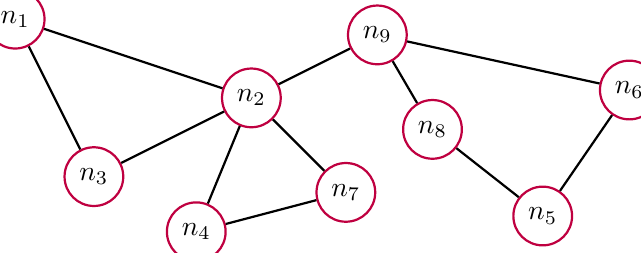
\begin{tikzpicture}[remember picture]
    \tikzstyle{edge}  = [thick,>=stealth,draw=black]
    \tikzstyle{dedge} = [thick,->,>=stealth,draw=black]
    \tikzstyle{node}=[
      overlay,
      circle,
      draw=purple,
      anchor=center,
      thick,
      minimum size=1,
    ]
    
    \node[node] (n1) at (-4,0) {$n_1$};
    \node[node] (n2) at (-1,-1) {$n_2$};
    \node[node] (n3) at (-3,-2) {$n_3$};
    \node[node] (n4) at (-1.7,-2.7) {$n_4$};
    \node[node] (n5) at (2.7,-2.5) {$n_5$};
    \node[node] (n6) at (3.8,-0.9) {$n_6$};
    \node[node] (n7) at (0.2,-2.2) {$n_7$};
    \node[node] (n8) at (1.3,-1.4) {$n_8$};
    \node[node] (n9) at (0.6,-0.2) {$n_9$};
    
    \draw[edge] (n1)--(n2);
    \draw[edge] (n2)--(n3);
    \draw[edge] (n1)--(n3);
    \draw[edge] (n2)--(n4);
    \draw[edge] (n2)--(n9);
    \draw[edge] (n9)--(n8);
    \draw[edge] (n6)--(n9);
    \draw[edge] (n5)--(n6);
    \draw[edge] (n2)--(n7);
    \draw[edge] (n7)--(n4);
    \draw[edge] (n8)--(n5);
  \end{tikzpicture}
\end{center}

  \caption{Example of a graph.}
  \label{fig:bs:graphs:graph}
\end{figure}

\begin{figure}[tbp]
  \begin{center}
  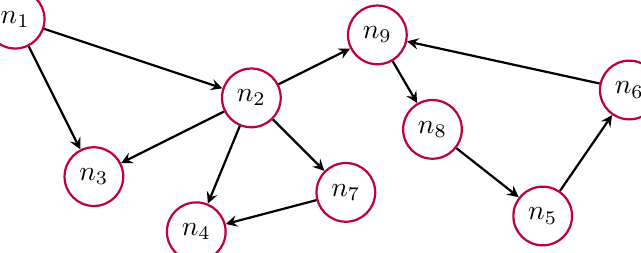
\begin{tikzpicture}[remember picture]
    \tikzstyle{edge}  = [thick,>=stealth,draw=black]
    \tikzstyle{dedge} = [thick,->,>=stealth,draw=black]
    \tikzstyle{node}=[
      overlay,
      circle,
      draw=purple,
      anchor=center,
      thick,
      minimum size=1,
    ]
    
    \node[node] (n1) at (-4,0) {$n_1$};
    \node[node] (n2) at (-1,-1) {$n_2$};
    \node[node] (n3) at (-3,-2) {$n_3$};
    \node[node] (n4) at (-1.7,-2.7) {$n_4$};
    \node[node] (n5) at (2.7,-2.5) {$n_5$};
    \node[node] (n6) at (3.8,-0.9) {$n_6$};
    \node[node] (n7) at (0.2,-2.2) {$n_7$};
    \node[node] (n8) at (1.3,-1.4) {$n_8$};
    \node[node] (n9) at (0.6,-0.2) {$n_9$};
    
    \draw[dedge] (n1)--(n2);
    \draw[dedge] (n2)--(n3);
    \draw[dedge] (n1)--(n3);
    \draw[dedge] (n2)--(n4);
    \draw[dedge] (n2)--(n9);
    \draw[dedge] (n9)--(n8);
    \draw[dedge] (n6)--(n9);
    \draw[dedge] (n5)--(n6);
    \draw[dedge] (n2)--(n7);
    \draw[dedge] (n7)--(n4);
    \draw[dedge] (n8)--(n5);
  \end{tikzpicture}
\end{center}

  \caption{Example of a directed graph.}
  \label{fig:bs:graphs:directed}
\end{figure}

\begin{figure}[tbp]
  \begin{center}
  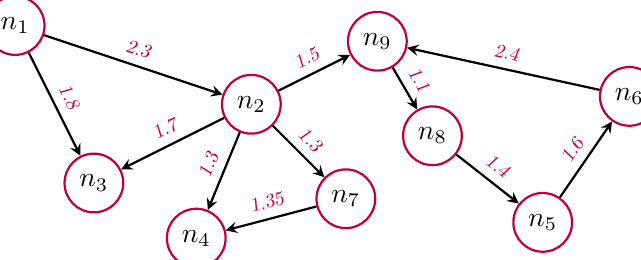
\begin{tikzpicture}[remember picture]
    \newcommand{\weight}[1]{node[midway,sloped,above] {\scalebox{0.7}{\textsl{\textcolor{purple}{#1}}}}}
    
    \tikzstyle{edge}  = [thick,>=stealth,draw=black]
    \tikzstyle{dedge} = [thick,->,>=stealth,draw=black]
    \tikzstyle{node}=[
      overlay,
      circle,
      draw=purple,
      anchor=center,
      thick,
      minimum size=1,
    ]
    
    \node[node] (n1) at (-4,0) {$n_1$};
    \node[node] (n2) at (-1,-1) {$n_2$};
    \node[node] (n3) at (-3,-2) {$n_3$};
    \node[node] (n4) at (-1.7,-2.7) {$n_4$};
    \node[node] (n5) at (2.7,-2.5) {$n_5$};
    \node[node] (n6) at (3.8,-0.9) {$n_6$};
    \node[node] (n7) at (0.2,-2.2) {$n_7$};
    \node[node] (n8) at (1.3,-1.4) {$n_8$};
    \node[node] (n9) at (0.6,-0.2) {$n_9$};
    
    \draw[dedge] (n1)--(n2) \weight{2.3};
    \draw[dedge] (n2)--(n3) \weight{1.7};
    \draw[dedge] (n1)--(n3) \weight{1.8};
    \draw[dedge] (n2)--(n4) \weight{1.3};
    \draw[dedge] (n2)--(n9) \weight{1.5};
    \draw[dedge] (n9)--(n8) \weight{1.1};
    \draw[dedge] (n6)--(n9) \weight{2.4};
    \draw[dedge] (n5)--(n6) \weight{1.6};
    \draw[dedge] (n2)--(n7) \weight{1.3};
    \draw[dedge] (n7)--(n4) \weight{1.35};
    \draw[dedge] (n8)--(n5) \weight{1.4};
  \end{tikzpicture}
\end{center}

  \caption{Example of a weighted graph.}
  \label{fig:bs:graphs:weighted}
\end{figure}

\begin{figure}[tbp]
  \begin{center}
  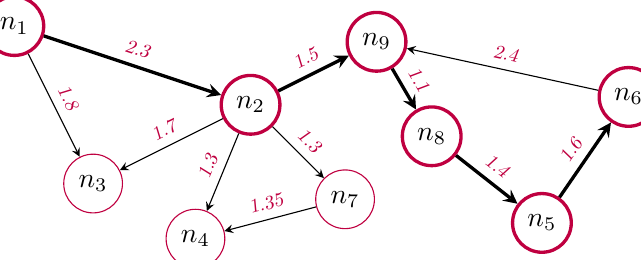
\begin{tikzpicture}[remember picture]
    \newcommand{\weight}[1]{node[midway,sloped,above] {\scalebox{0.7}{\textsl{\textcolor{purple}{#1}}}}}
    
    \tikzstyle{edge}  = [thick,>=stealth,draw=black]
    \tikzstyle{dedge} = [thick,->,>=stealth,draw=black]
    \tikzstyle{node}=[
      overlay,
      circle,
      draw=purple,
      anchor=center,
      thick,
      minimum size=1,
    ]
    
    \node[node,very thick] (n1) at (-4,0) {$n_1$};
    \node[node,very thick] (n2) at (-1,-1) {$n_2$};
    \node[node,thin] (n3) at (-3,-2) {$n_3$};
    \node[node,thin] (n4) at (-1.7,-2.7) {$n_4$};
    \node[node,very thick] (n5) at (2.7,-2.5) {$n_5$};
    \node[node,very thick] (n6) at (3.8,-0.9) {$n_6$};
    \node[node,thin] (n7) at (0.2,-2.2) {$n_7$};
    \node[node,very thick] (n8) at (1.3,-1.4) {$n_8$};
    \node[node,very thick] (n9) at (0.6,-0.2) {$n_9$};
    
    \draw[dedge,very thick] (n1)--(n2) \weight{2.3};
    \draw[dedge,thin] (n2)--(n3) \weight{1.7};
    \draw[dedge,thin] (n1)--(n3) \weight{1.8};
    \draw[dedge,thin] (n2)--(n4) \weight{1.3};
    \draw[dedge,very thick] (n2)--(n9) \weight{1.5};
    \draw[dedge,very thick] (n9)--(n8) \weight{1.1};
    \draw[dedge,thin] (n6)--(n9) \weight{2.4};
    \draw[dedge,very thick] (n5)--(n6) \weight{1.6};
    \draw[dedge,thin] (n2)--(n7) \weight{1.3};
    \draw[dedge,thin] (n7)--(n4) \weight{1.35};
    \draw[dedge,very thick] (n8)--(n5) \weight{1.4};
  \end{tikzpicture}
\end{center}

  \caption{Example of a path in a graph.}
  \label{fig:bs:graphs:path}
\end{figure}

\begin{figure}[tbp]
  \begin{center}
  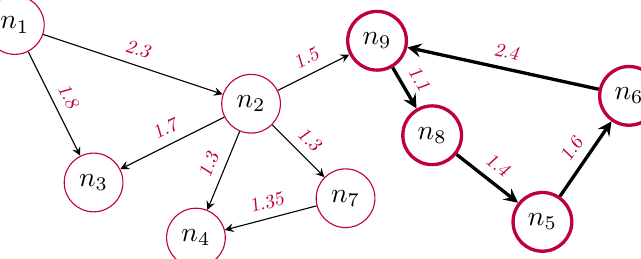
\begin{tikzpicture}[remember picture]
    \newcommand{\weight}[1]{node[midway,sloped,above] {\scalebox{0.7}{\textsl{\textcolor{purple}{#1}}}}}
    \tikzstyle{edge}  = [thick,>=stealth,draw=black]
    \tikzstyle{dedge} = [thick,->,>=stealth,draw=black]
    \tikzstyle{node}=[
      overlay,
      circle,
      draw=purple,
      anchor=center,
      thick,
      minimum size=1,
    ]
    
    \node[node,thin] (n1) at (-4,0) {$n_1$};
    \node[node,thin] (n2) at (-1,-1) {$n_2$};
    \node[node,thin] (n3) at (-3,-2) {$n_3$};
    \node[node,thin] (n4) at (-1.7,-2.7) {$n_4$};
    \node[node,very thick] (n5) at (2.7,-2.5) {$n_5$};
    \node[node,very thick] (n6) at (3.8,-0.9) {$n_6$};
    \node[node,thin] (n7) at (0.2,-2.2) {$n_7$};
    \node[node,very thick] (n8) at (1.3,-1.4) {$n_8$};
    \node[node,very thick] (n9) at (0.6,-0.2) {$n_9$};
    
    \draw[dedge,thin] (n1)--(n2) \weight{2.3};
    \draw[dedge,thin] (n2)--(n3) \weight{1.7};
    \draw[dedge,thin] (n1)--(n3) \weight{1.8};
    \draw[dedge,thin] (n2)--(n4) \weight{1.3};
    \draw[dedge,thin] (n2)--(n9) \weight{1.5};
    \draw[dedge,very thick] (n9)--(n8) \weight{1.1};
    \draw[dedge,very thick] (n6)--(n9) \weight{2.4};
    \draw[dedge,very thick] (n5)--(n6) \weight{1.6};
    \draw[dedge,thin] (n2)--(n7) \weight{1.3};
    \draw[dedge,thin] (n7)--(n4) \weight{1.35};
    \draw[dedge,very thick] (n8)--(n5) \weight{1.4};
  \end{tikzpicture}
\end{center}

  \caption{Example of a cycle in a graph.}
  \label{fig:bs:graphs:cycle}
\end{figure}

\begin{figure}[tbp]
  \begin{center}
  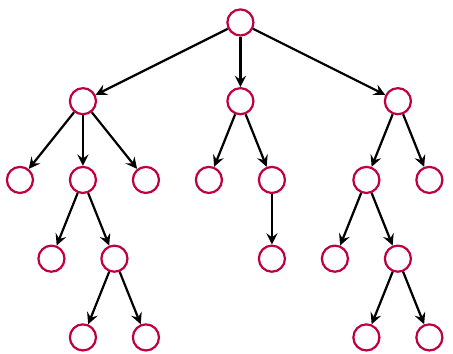
\begin{tikzpicture}[remember picture]
    \newcommand{\weight}[1]{node[midway,sloped,above] {\scalebox{0.7}{\textsl{\textcolor{purple}{#1}}}}}
    
    \tikzstyle{edge}  = [thick,>=stealth,draw=black]
    \tikzstyle{dedge} = [thick,->,>=stealth,draw=black]
    \tikzstyle{snode}=[
      overlay,
      circle,
      draw=purple,
      anchor=center,
      thick,
      minimum size=0.2,
    ]
    \tikzstyle{snoded}=[
      snode,
      rectangle,
      minimum width=0.3cm,
      minimum height=0.3cm,
    ]
    \tikzstyle{leaf}=[
      snode,
      draw=green!60!black,
    ]
    
    {
      \node[snode] (n1) at (0,0) {};
      
      \node[snode] (n11) at (-2.0,-1) {};
      \node[snode] (n12) at (0,-1) {};
      \node[snode] (n13) at (2.0,-1) {};
      
      \node[snode] (n111) at (-2.8,-2) {};
      \node[snode] (n112) at (-2.0,-2) {};
      \node[snode] (n113) at (-1.2,-2) {};
      \node[snode] (n121) at (-0.4,-2) {};
      \node[snode] (n122) at (0.4,-2) {};
      \node[snode] (n131) at (1.6,-2) {};
      \node[snode] (n132) at (2.4,-2) {};
      
      \node[snode] (n1121) at (-2.4,-3) {};
      \node[snode] (n1122) at (-1.6,-3) {};
      \node[snode] (n1221) at (0.4,-3) {};
      \node[snode] (n1311) at (1.2,-3) {};
      \node[snode] (n1312) at (2.0,-3) {};
      
      \node[snode] (n11221) at (-2.0,-4) {};
      \node[snode] (n11222) at (-1.2,-4) {};
      \node[snode] (n13121) at (1.6,-4) {};
      \node[snode] (n13122) at (2.4,-4) {};
    }
    
    {
      \draw[dedge] (n1)--(n11);
      \draw[dedge] (n1)--(n12);
      \draw[dedge] (n1)--(n13);
      
      \draw[dedge] (n11)--(n111);
      \draw[dedge] (n11)--(n112);
      \draw[dedge] (n11)--(n113);
      \draw[dedge] (n12)--(n121);
      \draw[dedge] (n12)--(n122);
      \draw[dedge] (n13)--(n131);
      \draw[dedge] (n13)--(n132);
      
      \draw[dedge] (n112)--(n1121);
      \draw[dedge] (n112)--(n1122);
      \draw[dedge] (n122)--(n1221);
      \draw[dedge] (n131)--(n1311);
      \draw[dedge] (n131)--(n1312);
      
      \draw[dedge] (n1122)--(n11221);
      \draw[dedge] (n1122)--(n11222);
      \draw[dedge] (n1312)--(n13121);
      \draw[dedge] (n1312)--(n13122);
    }
  \end{tikzpicture}
\end{center}

  \caption{Example of a tree.}
  \label{fig:bs:graphs:trees}
\end{figure}

\begin{figure}[tbp]
  \begin{center}
  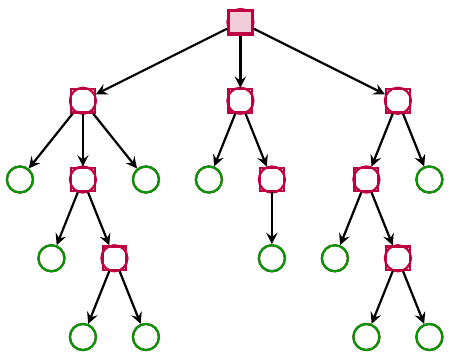
\begin{tikzpicture}[remember picture]
    \newcommand{\weight}[1]{node[midway,sloped,above] {\scalebox{0.7}{\textsl{\textcolor{purple}{#1}}}}}
    
    \tikzstyle{edge}  = [thick,>=stealth,draw=black]
    \tikzstyle{dedge} = [thick,->,>=stealth,draw=black]
    \tikzstyle{snode}=[
      overlay,
      circle,
      draw=purple,
      anchor=center,
      thick,
      minimum size=0.2,
    ]
    \tikzstyle{snoded}=[
      snode,
      rectangle,
      minimum width=0.3cm,
      minimum height=0.3cm,
    ]
    \tikzstyle{leaf}=[
      snode,
      draw=green!60!black,
    ]
    
    {
      \node[snode] (n1) at (0,0) {};
      
      \node[snode] (n11) at (-2.0,-1) {};
      \node[snode] (n12) at (0,-1) {};
      \node[snode] (n13) at (2.0,-1) {};
      
      \node[snode] (n111) at (-2.8,-2) {};
      \node[snode] (n112) at (-2.0,-2) {};
      \node[snode] (n113) at (-1.2,-2) {};
      \node[snode] (n121) at (-0.4,-2) {};
      \node[snode] (n122) at (0.4,-2) {};
      \node[snode] (n131) at (1.6,-2) {};
      \node[snode] (n132) at (2.4,-2) {};
      
      \node[snode] (n1121) at (-2.4,-3) {};
      \node[snode] (n1122) at (-1.6,-3) {};
      \node[snode] (n1221) at (0.4,-3) {};
      \node[snode] (n1311) at (1.2,-3) {};
      \node[snode] (n1312) at (2.0,-3) {};
      
      \node[snode] (n11221) at (-2.0,-4) {};
      \node[snode] (n11222) at (-1.2,-4) {};
      \node[snode] (n13121) at (1.6,-4) {};
      \node[snode] (n13122) at (2.4,-4) {};
    }
    
    {
      \node[snoded, very thick,fill=purple!20] (n1) at (0,0) {};
    }
    
    {
      \node[snoded] (n11) at (-2.0,-1) {};
      \node[snoded] (n12) at (0,-1) {};
      \node[snoded] (n13) at (2.0,-1) {};
      
      \node[leaf] (n111) at (-2.8,-2) {};
      \node[snoded] (n112) at (-2.0,-2) {};
      \node[leaf] (n113) at (-1.2,-2) {};
      \node[leaf] (n121) at (-0.4,-2) {};
      \node[snoded] (n122) at (0.4,-2) {};
      \node[snoded] (n131) at (1.6,-2) {};
      \node[leaf] (n132) at (2.4,-2) {};
      
      \node[leaf] (n1121) at (-2.4,-3) {};
      \node[snoded] (n1122) at (-1.6,-3) {};
      \node[leaf] (n1221) at (0.4,-3) {};
      \node[leaf] (n1311) at (1.2,-3) {};
      \node[snoded] (n1312) at (2.0,-3) {};
      
      \node[leaf] (n11221) at (-2.0,-4) {};
      \node[leaf] (n11222) at (-1.2,-4) {};
      \node[leaf] (n13121) at (1.6,-4) {};
      \node[leaf] (n13122) at (2.4,-4) {};
    }
    
    {
      \draw[dedge] (n1)--(n11);
      \draw[dedge] (n1)--(n12);
      \draw[dedge] (n1)--(n13);
      
      \draw[dedge] (n11)--(n111);
      \draw[dedge] (n11)--(n112);
      \draw[dedge] (n11)--(n113);
      \draw[dedge] (n12)--(n121);
      \draw[dedge] (n12)--(n122);
      \draw[dedge] (n13)--(n131);
      \draw[dedge] (n13)--(n132);
      
      \draw[dedge] (n112)--(n1121);
      \draw[dedge] (n112)--(n1122);
      \draw[dedge] (n122)--(n1221);
      \draw[dedge] (n131)--(n1311);
      \draw[dedge] (n131)--(n1312);
      
      \draw[dedge] (n1122)--(n11221);
      \draw[dedge] (n1122)--(n11222);
      \draw[dedge] (n1312)--(n13121);
      \draw[dedge] (n1312)--(n13122);
    }
  \end{tikzpicture}
\end{center}

  \caption{ENode types of a tree.}
  \label{fig:bs:graphs:trees:nodetypes}
\end{figure}


\section{Filesystems}

\begin{figure}[tbp]
  \begin{center}
  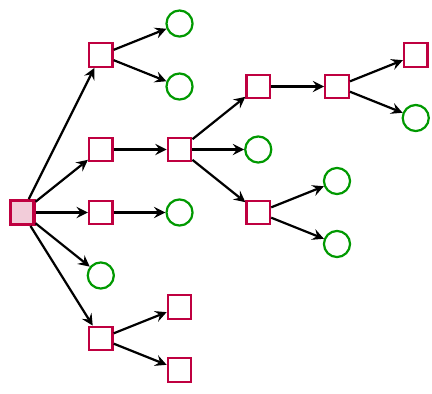
\begin{tikzpicture}[remember picture]
    \newcommand{\weight}[1]{node[midway,sloped,above] {\scalebox{0.7}{\textsl{\textcolor{purple}{#1}}}}}
    \tikzstyle{edge}  = [thick,>=stealth,draw=black]
    \tikzstyle{dedge} = [thick,->,>=stealth,draw=black]
    \tikzstyle{node}=[
      overlay,
      circle,
      draw=purple,
      anchor=center,
      thick,
      minimum size=0.2,
    ]
    \tikzstyle{dir}=[
      node,
      rectangle,
      minimum width=0.3cm,
      minimum height=0.3cm,
    ]
    \tikzstyle{file}=[
      node,
      draw=green!60!black,
    ]
    \tikzstyle{dirhighlight}=[
      dir,
      very thick,
      pattern=north east lines,
      pattern color=purple!60,
      even odd rule,
    ]
    \tikzstyle{filehighlight}=[
      file,
      very thick,
      pattern=north east lines,
      pattern color=green!60!black,
      even odd rule,
    ]
    
    \coordinate (rootAnchor) at (-5,-2);
    \coordinate (guestAnchor) at ([xshift=7cm, yshift=-1.2cm] rootAnchor);
    
    % root filesystem
    {
      \node[dir, very thick,fill=purple!20] (root1) at ([xshift=0cm, yshift=0cm] rootAnchor) {};
      
      \node[dir] (root11) at ([xshift=1cm, yshift=2.0cm] rootAnchor) {};
      \node[dir] (root12) at ([xshift=1cm, yshift=0.8cm] rootAnchor) {};
      \node[dir] (root13) at ([xshift=1cm, yshift=0.0cm] rootAnchor) {};
      \node[file] (root14) at ([xshift=1cm, yshift=-0.8cm] rootAnchor) {};
      \node[dir] (root15) at ([xshift=1cm, yshift=-1.6cm] rootAnchor) {};
      
      \node[file] (root111) at ([xshift=2cm, yshift=2.4cm] rootAnchor) {};
      \node[file] (root112) at ([xshift=2cm, yshift=1.6cm] rootAnchor) {};
      \node[dir] (root121) at ([xshift=2cm, yshift=0.8cm] rootAnchor) {};
      \node[file] (root131) at ([xshift=2cm, yshift=0.0cm] rootAnchor) {};
      \node[dir] (root151) at ([xshift=2cm, yshift=-1.2cm] rootAnchor) {};
      \node[dir] (root152) at ([xshift=2cm, yshift=-2.0cm] rootAnchor) {};
      
      \node[dir] (root1211) at ([xshift=3cm, yshift=1.6cm] rootAnchor) {};
      \node[file] (root1212) at ([xshift=3cm, yshift=0.8cm] rootAnchor) {};
      \node[dir] (root1213) at ([xshift=3cm, yshift=0.0cm] rootAnchor) {};
      
      \node[dir] (root12111) at ([xshift=4cm, yshift=1.6cm] rootAnchor) {};
      \node[file] (root12131) at ([xshift=4cm, yshift=0.4cm] rootAnchor) {};
      \node[file] (root12132) at ([xshift=4cm, yshift=-0.4cm] rootAnchor) {};
      
      \node[dir] (root121111) at ([xshift=5cm, yshift=2.0cm] rootAnchor) {};
      \node[file] (root121112) at ([xshift=5cm, yshift=1.2cm] rootAnchor) {};
      
      \draw[dedge] (root1)--(root11);
      \draw[dedge] (root1)--(root12);
      \draw[dedge] (root1)--(root13);
      \draw[dedge] (root1)--(root14);
      \draw[dedge] (root1)--(root15);
      
      \draw[dedge] (root11)--(root111);
      \draw[dedge] (root11)--(root112);
      \draw[dedge] (root12)--(root121);
      \draw[dedge] (root13)--(root131);
      \draw[dedge] (root15)--(root151);
      \draw[dedge] (root15)--(root152);
      
      \draw[dedge] (root121)--(root1211);
      \draw[dedge] (root121)--(root1212);
      \draw[dedge] (root121)--(root1213);
      
      \draw[dedge] (root1211)--(root12111);
      \draw[dedge] (root1213)--(root12131);
      \draw[dedge] (root1213)--(root12132);
      
      \draw[dedge] (root12111)--(root121111);
      \draw[dedge] (root12111)--(root121112);
    }
  \end{tikzpicture}
\end{center}

  \caption{Example of a filesystem.}
  \label{fig:bs:fs}
\end{figure}

\begin{figure}[tbp]
  \begin{center}
  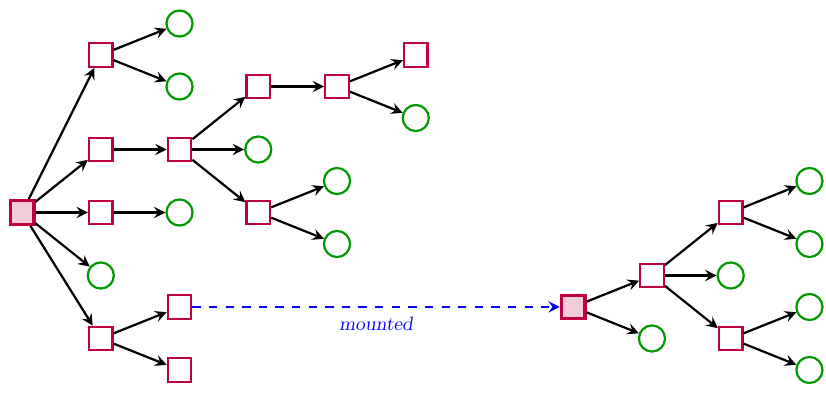
\begin{tikzpicture}[remember picture]
    \newcommand{\weight}[1]{node[midway,sloped,above] {\scalebox{0.7}{\textsl{\textcolor{purple}{#1}}}}}
    \tikzstyle{edge}  = [thick,>=stealth,draw=black]
    \tikzstyle{dedge} = [thick,->,>=stealth,draw=black]
    \tikzstyle{node}=[
      overlay,
      circle,
      draw=purple,
      anchor=center,
      thick,
      minimum size=0.2,
    ]
    \tikzstyle{dir}=[
      node,
      rectangle,
      minimum width=0.3cm,
      minimum height=0.3cm,
    ]
    \tikzstyle{file}=[
      node,
      draw=green!60!black,
    ]
    \tikzstyle{dirhighlight}=[
      dir,
      very thick,
      pattern=north east lines,
      pattern color=purple!60,
      even odd rule,
    ]
    \tikzstyle{filehighlight}=[
      file,
      very thick,
      pattern=north east lines,
      pattern color=green!60!black,
      even odd rule,
    ]
    
    \coordinate (rootAnchor) at (-5,-2);
    \coordinate (guestAnchor) at ([xshift=7cm, yshift=-1.2cm] rootAnchor);
    
    % root filesystem
    {
      \node[dir, very thick,fill=purple!20] (root1) at ([xshift=0cm, yshift=0cm] rootAnchor) {};
      
      \node[dir] (root11) at ([xshift=1cm, yshift=2.0cm] rootAnchor) {};
      \node[dir] (root12) at ([xshift=1cm, yshift=0.8cm] rootAnchor) {};
      \node[dir] (root13) at ([xshift=1cm, yshift=0.0cm] rootAnchor) {};
      \node[file] (root14) at ([xshift=1cm, yshift=-0.8cm] rootAnchor) {};
      \node[dir] (root15) at ([xshift=1cm, yshift=-1.6cm] rootAnchor) {};
      
      \node[file] (root111) at ([xshift=2cm, yshift=2.4cm] rootAnchor) {};
      \node[file] (root112) at ([xshift=2cm, yshift=1.6cm] rootAnchor) {};
      \node[dir] (root121) at ([xshift=2cm, yshift=0.8cm] rootAnchor) {};
      \node[file] (root131) at ([xshift=2cm, yshift=0.0cm] rootAnchor) {};
      \node[dir] (root151) at ([xshift=2cm, yshift=-1.2cm] rootAnchor) {};
      \node[dir] (root152) at ([xshift=2cm, yshift=-2.0cm] rootAnchor) {};
      
      \node[dir] (root1211) at ([xshift=3cm, yshift=1.6cm] rootAnchor) {};
      \node[file] (root1212) at ([xshift=3cm, yshift=0.8cm] rootAnchor) {};
      \node[dir] (root1213) at ([xshift=3cm, yshift=0.0cm] rootAnchor) {};
      
      \node[dir] (root12111) at ([xshift=4cm, yshift=1.6cm] rootAnchor) {};
      \node[file] (root12131) at ([xshift=4cm, yshift=0.4cm] rootAnchor) {};
      \node[file] (root12132) at ([xshift=4cm, yshift=-0.4cm] rootAnchor) {};
      
      \node[dir] (root121111) at ([xshift=5cm, yshift=2.0cm] rootAnchor) {};
      \node[file] (root121112) at ([xshift=5cm, yshift=1.2cm] rootAnchor) {};
      
      \draw[dedge] (root1)--(root11);
      \draw[dedge] (root1)--(root12);
      \draw[dedge] (root1)--(root13);
      \draw[dedge] (root1)--(root14);
      \draw[dedge] (root1)--(root15);
      
      \draw[dedge] (root11)--(root111);
      \draw[dedge] (root11)--(root112);
      \draw[dedge] (root12)--(root121);
      \draw[dedge] (root13)--(root131);
      \draw[dedge] (root15)--(root151);
      \draw[dedge] (root15)--(root152);
      
      \draw[dedge] (root121)--(root1211);
      \draw[dedge] (root121)--(root1212);
      \draw[dedge] (root121)--(root1213);
      
      \draw[dedge] (root1211)--(root12111);
      \draw[dedge] (root1213)--(root12131);
      \draw[dedge] (root1213)--(root12132);
      
      \draw[dedge] (root12111)--(root121111);
      \draw[dedge] (root12111)--(root121112);
    }
    
    % guest filesystem
    {
      \node[dir, very thick, fill=purple!20] (guest1) at ([xshift=0cm, yshift=0cm] guestAnchor) {};
      
      \node[dir] (guest11) at ([xshift=1cm, yshift=0.4cm] guestAnchor) {};
      \node[file] (guest12) at ([xshift=1cm, yshift=-0.4cm] guestAnchor) {};
      
      \node[dir] (guest111) at ([xshift=2cm, yshift=1.2cm] guestAnchor) {};
      \node[file] (guest112) at ([xshift=2cm, yshift=0.4cm] guestAnchor) {};
      \node[dir] (guest113) at ([xshift=2cm, yshift=-0.4cm] guestAnchor) {};
      
      \node[file] (guest1111) at ([xshift=3cm, yshift=1.6cm] guestAnchor) {};
      \node[file] (guest1112) at ([xshift=3cm, yshift=0.8cm] guestAnchor) {};
      \node[file] (guest1131) at ([xshift=3cm, yshift=0.0cm] guestAnchor) {};
      \node[file] (guest1132) at ([xshift=3cm, yshift=-0.8cm] guestAnchor) {};
      
      \draw[dedge] (guest1)--(guest11);
      \draw[dedge] (guest1)--(guest12);
      
      \draw[dedge] (guest11)--(guest111);
      \draw[dedge] (guest11)--(guest112);
      \draw[dedge] (guest11)--(guest113);
      
      \draw[dedge] (guest111)--(guest1111);
      \draw[dedge] (guest111)--(guest1112);
      \draw[dedge] (guest113)--(guest1131);
      \draw[dedge] (guest113)--(guest1132);
    }
    
    % mount
    {
      \draw[dedge, dashed, draw=blue] (root151)--(guest1) node[midway,sloped,below] {\scalebox{0.7}{\textsl{\textcolor{blue}{mounted}}}};
    }
  \end{tikzpicture}
\end{center}

  \caption{Example of a mounting a guest filesystem.}
  \label{fig:bs:fs:mounting}
\end{figure}

\begin{figure}[tbp]
  \begin{center}
  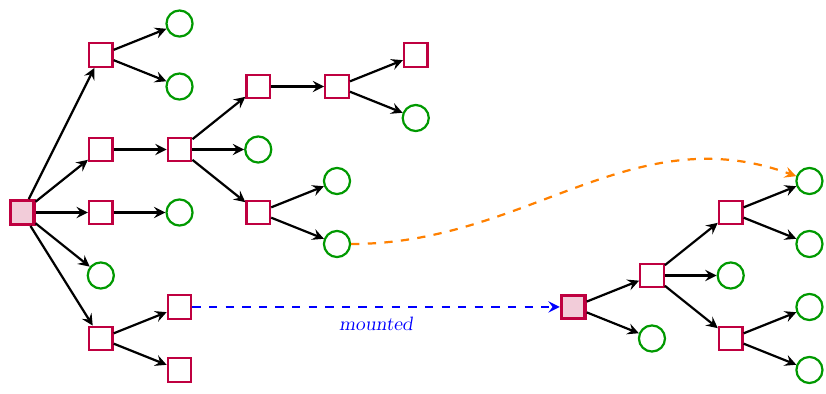
\begin{tikzpicture}[remember picture]
    \newcommand{\weight}[1]{node[midway,sloped,above] {\scalebox{0.7}{\textsl{\textcolor{purple}{#1}}}}}
    \tikzstyle{edge}  = [thick,>=stealth,draw=black]
    \tikzstyle{dedge} = [thick,->,>=stealth,draw=black]
    \tikzstyle{node}=[
      overlay,
      circle,
      draw=purple,
      anchor=center,
      thick,
      minimum size=0.2,
    ]
    \tikzstyle{dir}=[
      node,
      rectangle,
      minimum width=0.3cm,
      minimum height=0.3cm,
    ]
    \tikzstyle{file}=[
      node,
      draw=green!60!black,
    ]
    \tikzstyle{dirhighlight}=[
      dir,
      very thick,
      pattern=north east lines,
      pattern color=purple!60,
      even odd rule,
    ]
    \tikzstyle{filehighlight}=[
      file,
      very thick,
      pattern=north east lines,
      pattern color=green!60!black,
      even odd rule,
    ]
    
    \coordinate (rootAnchor) at (-5,-2);
    \coordinate (guestAnchor) at ([xshift=7cm, yshift=-1.2cm] rootAnchor);
    
    % root filesystem
    {
      \node[dir, very thick,fill=purple!20] (root1) at ([xshift=0cm, yshift=0cm] rootAnchor) {};
      
      \node[dir] (root11) at ([xshift=1cm, yshift=2.0cm] rootAnchor) {};
      \node[dir] (root12) at ([xshift=1cm, yshift=0.8cm] rootAnchor) {};
      \node[dir] (root13) at ([xshift=1cm, yshift=0.0cm] rootAnchor) {};
      \node[file] (root14) at ([xshift=1cm, yshift=-0.8cm] rootAnchor) {};
      \node[dir] (root15) at ([xshift=1cm, yshift=-1.6cm] rootAnchor) {};
      
      \node[file] (root111) at ([xshift=2cm, yshift=2.4cm] rootAnchor) {};
      \node[file] (root112) at ([xshift=2cm, yshift=1.6cm] rootAnchor) {};
      \node[dir] (root121) at ([xshift=2cm, yshift=0.8cm] rootAnchor) {};
      \node[file] (root131) at ([xshift=2cm, yshift=0.0cm] rootAnchor) {};
      \node[dir] (root151) at ([xshift=2cm, yshift=-1.2cm] rootAnchor) {};
      \node[dir] (root152) at ([xshift=2cm, yshift=-2.0cm] rootAnchor) {};
      
      \node[dir] (root1211) at ([xshift=3cm, yshift=1.6cm] rootAnchor) {};
      \node[file] (root1212) at ([xshift=3cm, yshift=0.8cm] rootAnchor) {};
      \node[dir] (root1213) at ([xshift=3cm, yshift=0.0cm] rootAnchor) {};
      
      \node[dir] (root12111) at ([xshift=4cm, yshift=1.6cm] rootAnchor) {};
      \node[file] (root12131) at ([xshift=4cm, yshift=0.4cm] rootAnchor) {};
      \node[file] (root12132) at ([xshift=4cm, yshift=-0.4cm] rootAnchor) {};
      
      \node[dir] (root121111) at ([xshift=5cm, yshift=2.0cm] rootAnchor) {};
      \node[file] (root121112) at ([xshift=5cm, yshift=1.2cm] rootAnchor) {};
      
      \draw[dedge] (root1)--(root11);
      \draw[dedge] (root1)--(root12);
      \draw[dedge] (root1)--(root13);
      \draw[dedge] (root1)--(root14);
      \draw[dedge] (root1)--(root15);
      
      \draw[dedge] (root11)--(root111);
      \draw[dedge] (root11)--(root112);
      \draw[dedge] (root12)--(root121);
      \draw[dedge] (root13)--(root131);
      \draw[dedge] (root15)--(root151);
      \draw[dedge] (root15)--(root152);
      
      \draw[dedge] (root121)--(root1211);
      \draw[dedge] (root121)--(root1212);
      \draw[dedge] (root121)--(root1213);
      
      \draw[dedge] (root1211)--(root12111);
      \draw[dedge] (root1213)--(root12131);
      \draw[dedge] (root1213)--(root12132);
      
      \draw[dedge] (root12111)--(root121111);
      \draw[dedge] (root12111)--(root121112);
    }
    
    % guest filesystem
    {
      \node[dir, very thick, fill=purple!20] (guest1) at ([xshift=0cm, yshift=0cm] guestAnchor) {};
      
      \node[dir] (guest11) at ([xshift=1cm, yshift=0.4cm] guestAnchor) {};
      \node[file] (guest12) at ([xshift=1cm, yshift=-0.4cm] guestAnchor) {};
      
      \node[dir] (guest111) at ([xshift=2cm, yshift=1.2cm] guestAnchor) {};
      \node[file] (guest112) at ([xshift=2cm, yshift=0.4cm] guestAnchor) {};
      \node[dir] (guest113) at ([xshift=2cm, yshift=-0.4cm] guestAnchor) {};
      
      \node[file] (guest1111) at ([xshift=3cm, yshift=1.6cm] guestAnchor) {};
      \node[file] (guest1112) at ([xshift=3cm, yshift=0.8cm] guestAnchor) {};
      \node[file] (guest1131) at ([xshift=3cm, yshift=0.0cm] guestAnchor) {};
      \node[file] (guest1132) at ([xshift=3cm, yshift=-0.8cm] guestAnchor) {};
      
      \draw[dedge] (guest1)--(guest11);
      \draw[dedge] (guest1)--(guest12);
      
      \draw[dedge] (guest11)--(guest111);
      \draw[dedge] (guest11)--(guest112);
      \draw[dedge] (guest11)--(guest113);
      
      \draw[dedge] (guest111)--(guest1111);
      \draw[dedge] (guest111)--(guest1112);
      \draw[dedge] (guest113)--(guest1131);
      \draw[dedge] (guest113)--(guest1132);
    }
    
    % mount
    {
      \draw[dedge, dashed, draw=blue] (root151)--(guest1) node[midway,sloped,below] {\scalebox{0.7}{\textsl{\textcolor{blue}{mounted}}}};
    }
    
    % link
    {
      \draw[dedge, dashed, draw=orange] (root12132) to [out=0,in=160] (guest1111);
    }
  \end{tikzpicture}
\end{center}

  \caption{Example of a link in a filesystem.}
  \label{fig:bs:fs:links}
\end{figure}

\begin{figure}[tbp]
  \begin{center}
  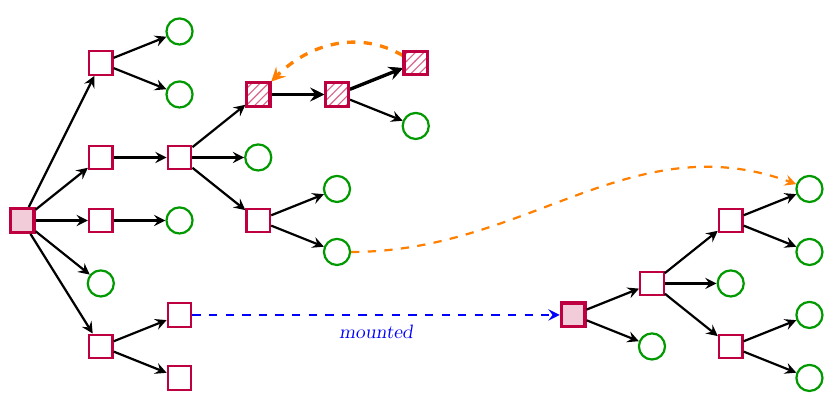
\begin{tikzpicture}[remember picture]
    \newcommand{\weight}[1]{node[midway,sloped,above] {\scalebox{0.7}{\textsl{\textcolor{purple}{#1}}}}}
    \tikzstyle{edge}  = [thick,>=stealth,draw=black]
    \tikzstyle{dedge} = [thick,->,>=stealth,draw=black]
    \tikzstyle{node}=[
      overlay,
      circle,
      draw=purple,
      anchor=center,
      thick,
      minimum size=0.2,
    ]
    \tikzstyle{dir}=[
      node,
      rectangle,
      minimum width=0.3cm,
      minimum height=0.3cm,
    ]
    \tikzstyle{file}=[
      node,
      draw=green!60!black,
    ]
    \tikzstyle{dirhighlight}=[
      dir,
      very thick,
      pattern=north east lines,
      pattern color=purple!60,
      even odd rule,
    ]
    \tikzstyle{filehighlight}=[
      file,
      very thick,
      pattern=north east lines,
      pattern color=green!60!black,
      even odd rule,
    ]
    
    \coordinate (rootAnchor) at (-5,-2);
    \coordinate (guestAnchor) at ([xshift=7cm, yshift=-1.2cm] rootAnchor);
    
    % root filesystem
    {
      \node[dir, very thick,fill=purple!20] (root1) at ([xshift=0cm, yshift=0cm] rootAnchor) {};
      
      \node[dir] (root11) at ([xshift=1cm, yshift=2.0cm] rootAnchor) {};
      \node[dir] (root12) at ([xshift=1cm, yshift=0.8cm] rootAnchor) {};
      \node[dir] (root13) at ([xshift=1cm, yshift=0.0cm] rootAnchor) {};
      \node[file] (root14) at ([xshift=1cm, yshift=-0.8cm] rootAnchor) {};
      \node[dir] (root15) at ([xshift=1cm, yshift=-1.6cm] rootAnchor) {};
      
      \node[file] (root111) at ([xshift=2cm, yshift=2.4cm] rootAnchor) {};
      \node[file] (root112) at ([xshift=2cm, yshift=1.6cm] rootAnchor) {};
      \node[dir] (root121) at ([xshift=2cm, yshift=0.8cm] rootAnchor) {};
      \node[file] (root131) at ([xshift=2cm, yshift=0.0cm] rootAnchor) {};
      \node[dir] (root151) at ([xshift=2cm, yshift=-1.2cm] rootAnchor) {};
      \node[dir] (root152) at ([xshift=2cm, yshift=-2.0cm] rootAnchor) {};
      
      \node[dir] (root1211) at ([xshift=3cm, yshift=1.6cm] rootAnchor) {};
      \node[file] (root1212) at ([xshift=3cm, yshift=0.8cm] rootAnchor) {};
      \node[dir] (root1213) at ([xshift=3cm, yshift=0.0cm] rootAnchor) {};
      
      \node[dir] (root12111) at ([xshift=4cm, yshift=1.6cm] rootAnchor) {};
      \node[file] (root12131) at ([xshift=4cm, yshift=0.4cm] rootAnchor) {};
      \node[file] (root12132) at ([xshift=4cm, yshift=-0.4cm] rootAnchor) {};
      
      \node[dir] (root121111) at ([xshift=5cm, yshift=2.0cm] rootAnchor) {};
      \node[file] (root121112) at ([xshift=5cm, yshift=1.2cm] rootAnchor) {};
      
      \draw[dedge] (root1)--(root11);
      \draw[dedge] (root1)--(root12);
      \draw[dedge] (root1)--(root13);
      \draw[dedge] (root1)--(root14);
      \draw[dedge] (root1)--(root15);
      
      \draw[dedge] (root11)--(root111);
      \draw[dedge] (root11)--(root112);
      \draw[dedge] (root12)--(root121);
      \draw[dedge] (root13)--(root131);
      \draw[dedge] (root15)--(root151);
      \draw[dedge] (root15)--(root152);
      
      \draw[dedge] (root121)--(root1211);
      \draw[dedge] (root121)--(root1212);
      \draw[dedge] (root121)--(root1213);
      
      \draw[dedge] (root1211)--(root12111);
      \draw[dedge] (root1213)--(root12131);
      \draw[dedge] (root1213)--(root12132);
      
      \draw[dedge] (root12111)--(root121111);
      \draw[dedge] (root12111)--(root121112);
    }
    
    % guest filesystem
    {
      \node[dir, very thick, fill=purple!20] (guest1) at ([xshift=0cm, yshift=0cm] guestAnchor) {};
      
      \node[dir] (guest11) at ([xshift=1cm, yshift=0.4cm] guestAnchor) {};
      \node[file] (guest12) at ([xshift=1cm, yshift=-0.4cm] guestAnchor) {};
      
      \node[dir] (guest111) at ([xshift=2cm, yshift=1.2cm] guestAnchor) {};
      \node[file] (guest112) at ([xshift=2cm, yshift=0.4cm] guestAnchor) {};
      \node[dir] (guest113) at ([xshift=2cm, yshift=-0.4cm] guestAnchor) {};
      
      \node[file] (guest1111) at ([xshift=3cm, yshift=1.6cm] guestAnchor) {};
      \node[file] (guest1112) at ([xshift=3cm, yshift=0.8cm] guestAnchor) {};
      \node[file] (guest1131) at ([xshift=3cm, yshift=0.0cm] guestAnchor) {};
      \node[file] (guest1132) at ([xshift=3cm, yshift=-0.8cm] guestAnchor) {};
      
      \draw[dedge] (guest1)--(guest11);
      \draw[dedge] (guest1)--(guest12);
      
      \draw[dedge] (guest11)--(guest111);
      \draw[dedge] (guest11)--(guest112);
      \draw[dedge] (guest11)--(guest113);
      
      \draw[dedge] (guest111)--(guest1111);
      \draw[dedge] (guest111)--(guest1112);
      \draw[dedge] (guest113)--(guest1131);
      \draw[dedge] (guest113)--(guest1132);
    }
    
    % mount
    {
      \draw[dedge, dashed, draw=blue] (root151)--(guest1) node[midway,sloped,below] {\scalebox{0.7}{\textsl{\textcolor{blue}{mounted}}}};
    }
    
    % link
    {
      \draw[dedge, dashed, draw=orange] (root12132) to [out=0,in=160] (guest1111);
    }
    
    % cycle link
    {
      \draw[dedge, dashed, draw=orange, very thick] (root121111) to [out=150,in=45] (root1211);
      \draw[dedge, very thick] (root1211)--(root12111);
      \draw[dedge, very thick] (root12111)--(root121111);
      \node[dirhighlight] (root1211) at ([xshift=3cm, yshift=1.6cm] rootAnchor) {};
      \node[dirhighlight] (root12111) at ([xshift=4cm, yshift=1.6cm] rootAnchor) {};
      \node[dirhighlight] (root121111) at ([xshift=5cm, yshift=2.0cm] rootAnchor) {};
    }
  \end{tikzpicture}
\end{center}

  \caption{Example of how a link can create a cycle in a filesystem.}
  \label{fig:bs:fs:cycles}
\end{figure}

\begin{figure}[tbp]
  \begin{center}
  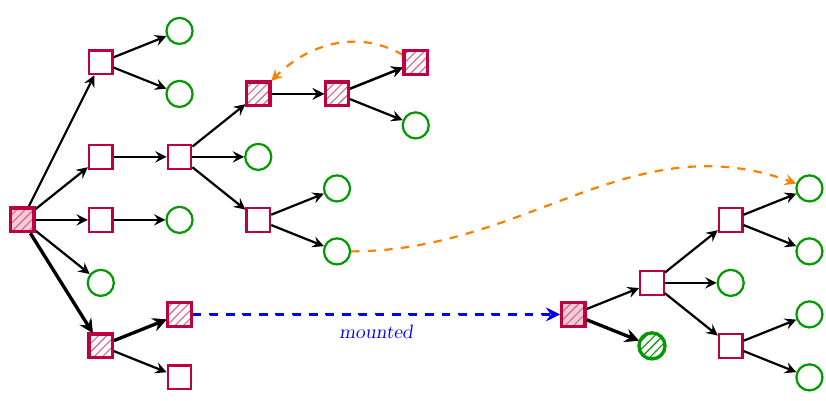
\begin{tikzpicture}[remember picture]
    \newcommand{\weight}[1]{node[midway,sloped,above] {\scalebox{0.7}{\textsl{\textcolor{purple}{#1}}}}}
    \tikzstyle{edge}  = [thick,>=stealth,draw=black]
    \tikzstyle{dedge} = [thick,->,>=stealth,draw=black]
    \tikzstyle{node}=[
      overlay,
      circle,
      draw=purple,
      anchor=center,
      thick,
      minimum size=0.2,
    ]
    \tikzstyle{dir}=[
      node,
      rectangle,
      minimum width=0.3cm,
      minimum height=0.3cm,
    ]
    \tikzstyle{file}=[
      node,
      draw=green!60!black,
    ]
    \tikzstyle{dirhighlight}=[
      dir,
      very thick,
      pattern=north east lines,
      pattern color=purple!60,
      even odd rule,
    ]
    \tikzstyle{filehighlight}=[
      file,
      very thick,
      pattern=north east lines,
      pattern color=green!60!black,
      even odd rule,
    ]
    
    \coordinate (rootAnchor) at (-5,-2);
    \coordinate (guestAnchor) at ([xshift=7cm, yshift=-1.2cm] rootAnchor);
    
    % root filesystem
    {
      \node[dir, very thick,fill=purple!20] (root1) at ([xshift=0cm, yshift=0cm] rootAnchor) {};
      
      \node[dir] (root11) at ([xshift=1cm, yshift=2.0cm] rootAnchor) {};
      \node[dir] (root12) at ([xshift=1cm, yshift=0.8cm] rootAnchor) {};
      \node[dir] (root13) at ([xshift=1cm, yshift=0.0cm] rootAnchor) {};
      \node[file] (root14) at ([xshift=1cm, yshift=-0.8cm] rootAnchor) {};
      \node[dir] (root15) at ([xshift=1cm, yshift=-1.6cm] rootAnchor) {};
      
      \node[file] (root111) at ([xshift=2cm, yshift=2.4cm] rootAnchor) {};
      \node[file] (root112) at ([xshift=2cm, yshift=1.6cm] rootAnchor) {};
      \node[dir] (root121) at ([xshift=2cm, yshift=0.8cm] rootAnchor) {};
      \node[file] (root131) at ([xshift=2cm, yshift=0.0cm] rootAnchor) {};
      \node[dir] (root151) at ([xshift=2cm, yshift=-1.2cm] rootAnchor) {};
      \node[dir] (root152) at ([xshift=2cm, yshift=-2.0cm] rootAnchor) {};
      
      \node[dir] (root1211) at ([xshift=3cm, yshift=1.6cm] rootAnchor) {};
      \node[file] (root1212) at ([xshift=3cm, yshift=0.8cm] rootAnchor) {};
      \node[dir] (root1213) at ([xshift=3cm, yshift=0.0cm] rootAnchor) {};
      
      \node[dir] (root12111) at ([xshift=4cm, yshift=1.6cm] rootAnchor) {};
      \node[file] (root12131) at ([xshift=4cm, yshift=0.4cm] rootAnchor) {};
      \node[file] (root12132) at ([xshift=4cm, yshift=-0.4cm] rootAnchor) {};
      
      \node[dir] (root121111) at ([xshift=5cm, yshift=2.0cm] rootAnchor) {};
      \node[file] (root121112) at ([xshift=5cm, yshift=1.2cm] rootAnchor) {};
      
      \draw[dedge] (root1)--(root11);
      \draw[dedge] (root1)--(root12);
      \draw[dedge] (root1)--(root13);
      \draw[dedge] (root1)--(root14);
      \draw[dedge] (root1)--(root15);
      
      \draw[dedge] (root11)--(root111);
      \draw[dedge] (root11)--(root112);
      \draw[dedge] (root12)--(root121);
      \draw[dedge] (root13)--(root131);
      \draw[dedge] (root15)--(root151);
      \draw[dedge] (root15)--(root152);
      
      \draw[dedge] (root121)--(root1211);
      \draw[dedge] (root121)--(root1212);
      \draw[dedge] (root121)--(root1213);
      
      \draw[dedge] (root1211)--(root12111);
      \draw[dedge] (root1213)--(root12131);
      \draw[dedge] (root1213)--(root12132);
      
      \draw[dedge] (root12111)--(root121111);
      \draw[dedge] (root12111)--(root121112);
    }
    
    % guest filesystem
    {
      \node[dir, very thick, fill=purple!20] (guest1) at ([xshift=0cm, yshift=0cm] guestAnchor) {};
      
      \node[dir] (guest11) at ([xshift=1cm, yshift=0.4cm] guestAnchor) {};
      \node[file] (guest12) at ([xshift=1cm, yshift=-0.4cm] guestAnchor) {};
      
      \node[dir] (guest111) at ([xshift=2cm, yshift=1.2cm] guestAnchor) {};
      \node[file] (guest112) at ([xshift=2cm, yshift=0.4cm] guestAnchor) {};
      \node[dir] (guest113) at ([xshift=2cm, yshift=-0.4cm] guestAnchor) {};
      
      \node[file] (guest1111) at ([xshift=3cm, yshift=1.6cm] guestAnchor) {};
      \node[file] (guest1112) at ([xshift=3cm, yshift=0.8cm] guestAnchor) {};
      \node[file] (guest1131) at ([xshift=3cm, yshift=0.0cm] guestAnchor) {};
      \node[file] (guest1132) at ([xshift=3cm, yshift=-0.8cm] guestAnchor) {};
      
      \draw[dedge] (guest1)--(guest11);
      \draw[dedge] (guest1)--(guest12);
      
      \draw[dedge] (guest11)--(guest111);
      \draw[dedge] (guest11)--(guest112);
      \draw[dedge] (guest11)--(guest113);
      
      \draw[dedge] (guest111)--(guest1111);
      \draw[dedge] (guest111)--(guest1112);
      \draw[dedge] (guest113)--(guest1131);
      \draw[dedge] (guest113)--(guest1132);
    }
    
    % mount
    {
      \draw[dedge, dashed, draw=blue] (root151)--(guest1) node[midway,sloped,below] {\scalebox{0.7}{\textsl{\textcolor{blue}{mounted}}}};
    }
    
    % link
    {
      \draw[dedge, dashed, draw=orange] (root12132) to [out=0,in=160] (guest1111);
    }
    
    % cycle link
    {
      \draw[dedge, dashed, draw=orange] (root121111) to [out=150,in=45] (root1211);
      \draw[dedge] (root1211)--(root12111);
      \draw[dedge] (root12111)--(root121111);
      \node[dirhighlight] (root1211) at ([xshift=3cm, yshift=1.6cm] rootAnchor) {};
      \node[dirhighlight] (root12111) at ([xshift=4cm, yshift=1.6cm] rootAnchor) {};
      \node[dirhighlight] (root121111) at ([xshift=5cm, yshift=2.0cm] rootAnchor) {};
    }
    
    % absolute path
    {
      \node[dirhighlight] (root1) at ([xshift=0cm, yshift=0cm] rootAnchor) {};
      \draw[dedge, very thick] (root1)--(root15);
      \node[dirhighlight] (root15) at ([xshift=1cm, yshift=-1.6cm] rootAnchor) {};
      \draw[dedge, very thick] (root15)--(root151);
      \node[dirhighlight] (root151) at ([xshift=2cm, yshift=-1.2cm] rootAnchor) {};
      \draw[dedge, dashed, draw=blue, very thick] (root151)--(guest1) node[midway,sloped,below] {};
      \node[dirhighlight] (guest1) at ([xshift=0cm, yshift=0cm] guestAnchor) {};
      \draw[dedge, very thick] (guest1)--(guest12);
      \node[filehighlight] (guest12) at ([xshift=1cm, yshift=-0.4cm] guestAnchor) {};
    }
  \end{tikzpicture}
\end{center}

  \caption{Example of an absolute path in a filesystem.}
  \label{fig:bs:fs:path:abs}
\end{figure}

\begin{figure}[tbp]
  \begin{center}
  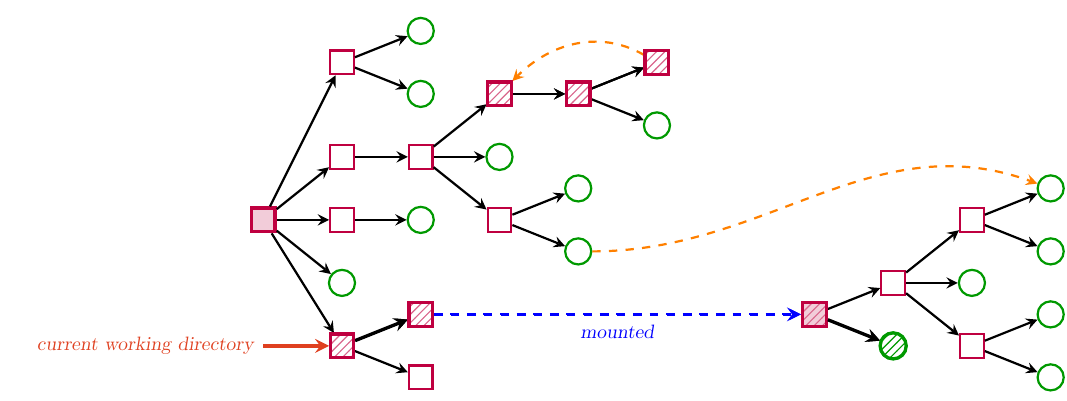
\begin{tikzpicture}[remember picture]
    \newcommand{\weight}[1]{node[midway,sloped,above] {\scalebox{0.7}{\textsl{\textcolor{purple}{#1}}}}}
    \tikzstyle{edge}  = [thick,>=stealth,draw=black]
    \tikzstyle{dedge} = [thick,->,>=stealth,draw=black]
    \tikzstyle{node}=[
      overlay,
      circle,
      draw=purple,
      anchor=center,
      thick,
      minimum size=0.2,
    ]
    \tikzstyle{dir}=[
      node,
      rectangle,
      minimum width=0.3cm,
      minimum height=0.3cm,
    ]
    \tikzstyle{file}=[
      node,
      draw=green!60!black,
    ]
    \tikzstyle{dirhighlight}=[
      dir,
      very thick,
      pattern=north east lines,
      pattern color=purple!60,
      even odd rule,
    ]
    \tikzstyle{filehighlight}=[
      file,
      very thick,
      pattern=north east lines,
      pattern color=green!60!black,
      even odd rule,
    ]
    
    \coordinate (rootAnchor) at (-5,-2);
    \coordinate (guestAnchor) at ([xshift=7cm, yshift=-1.2cm] rootAnchor);
    
    % root filesystem
    {
      \node[dir, very thick,fill=purple!20] (root1) at ([xshift=0cm, yshift=0cm] rootAnchor) {};
      
      \node[dir] (root11) at ([xshift=1cm, yshift=2.0cm] rootAnchor) {};
      \node[dir] (root12) at ([xshift=1cm, yshift=0.8cm] rootAnchor) {};
      \node[dir] (root13) at ([xshift=1cm, yshift=0.0cm] rootAnchor) {};
      \node[file] (root14) at ([xshift=1cm, yshift=-0.8cm] rootAnchor) {};
      \node[dir] (root15) at ([xshift=1cm, yshift=-1.6cm] rootAnchor) {};
      
      \node[file] (root111) at ([xshift=2cm, yshift=2.4cm] rootAnchor) {};
      \node[file] (root112) at ([xshift=2cm, yshift=1.6cm] rootAnchor) {};
      \node[dir] (root121) at ([xshift=2cm, yshift=0.8cm] rootAnchor) {};
      \node[file] (root131) at ([xshift=2cm, yshift=0.0cm] rootAnchor) {};
      \node[dir] (root151) at ([xshift=2cm, yshift=-1.2cm] rootAnchor) {};
      \node[dir] (root152) at ([xshift=2cm, yshift=-2.0cm] rootAnchor) {};
      
      \node[dir] (root1211) at ([xshift=3cm, yshift=1.6cm] rootAnchor) {};
      \node[file] (root1212) at ([xshift=3cm, yshift=0.8cm] rootAnchor) {};
      \node[dir] (root1213) at ([xshift=3cm, yshift=0.0cm] rootAnchor) {};
      
      \node[dir] (root12111) at ([xshift=4cm, yshift=1.6cm] rootAnchor) {};
      \node[file] (root12131) at ([xshift=4cm, yshift=0.4cm] rootAnchor) {};
      \node[file] (root12132) at ([xshift=4cm, yshift=-0.4cm] rootAnchor) {};
      
      \node[dir] (root121111) at ([xshift=5cm, yshift=2.0cm] rootAnchor) {};
      \node[file] (root121112) at ([xshift=5cm, yshift=1.2cm] rootAnchor) {};
      
      \draw[dedge] (root1)--(root11);
      \draw[dedge] (root1)--(root12);
      \draw[dedge] (root1)--(root13);
      \draw[dedge] (root1)--(root14);
      \draw[dedge] (root1)--(root15);
      
      \draw[dedge] (root11)--(root111);
      \draw[dedge] (root11)--(root112);
      \draw[dedge] (root12)--(root121);
      \draw[dedge] (root13)--(root131);
      \draw[dedge] (root15)--(root151);
      \draw[dedge] (root15)--(root152);
      
      \draw[dedge] (root121)--(root1211);
      \draw[dedge] (root121)--(root1212);
      \draw[dedge] (root121)--(root1213);
      
      \draw[dedge] (root1211)--(root12111);
      \draw[dedge] (root1213)--(root12131);
      \draw[dedge] (root1213)--(root12132);
      
      \draw[dedge] (root12111)--(root121111);
      \draw[dedge] (root12111)--(root121112);
    }
    
    % guest filesystem
    {
      \node[dir, very thick, fill=purple!20] (guest1) at ([xshift=0cm, yshift=0cm] guestAnchor) {};
      
      \node[dir] (guest11) at ([xshift=1cm, yshift=0.4cm] guestAnchor) {};
      \node[file] (guest12) at ([xshift=1cm, yshift=-0.4cm] guestAnchor) {};
      
      \node[dir] (guest111) at ([xshift=2cm, yshift=1.2cm] guestAnchor) {};
      \node[file] (guest112) at ([xshift=2cm, yshift=0.4cm] guestAnchor) {};
      \node[dir] (guest113) at ([xshift=2cm, yshift=-0.4cm] guestAnchor) {};
      
      \node[file] (guest1111) at ([xshift=3cm, yshift=1.6cm] guestAnchor) {};
      \node[file] (guest1112) at ([xshift=3cm, yshift=0.8cm] guestAnchor) {};
      \node[file] (guest1131) at ([xshift=3cm, yshift=0.0cm] guestAnchor) {};
      \node[file] (guest1132) at ([xshift=3cm, yshift=-0.8cm] guestAnchor) {};
      
      \draw[dedge] (guest1)--(guest11);
      \draw[dedge] (guest1)--(guest12);
      
      \draw[dedge] (guest11)--(guest111);
      \draw[dedge] (guest11)--(guest112);
      \draw[dedge] (guest11)--(guest113);
      
      \draw[dedge] (guest111)--(guest1111);
      \draw[dedge] (guest111)--(guest1112);
      \draw[dedge] (guest113)--(guest1131);
      \draw[dedge] (guest113)--(guest1132);
    }
    
    % mount
    {
      \draw[dedge, dashed, draw=blue] (root151)--(guest1) node[midway,sloped,below] {\scalebox{0.7}{\textsl{\textcolor{blue}{mounted}}}};
    }
    
    % link
    {
      \draw[dedge, dashed, draw=orange] (root12132) to [out=0,in=160] (guest1111);
    }
    
    % cycle link
    {
      \draw[dedge, dashed, draw=orange] (root121111) to [out=150,in=45] (root1211);
      \draw[dedge] (root1211)--(root12111);
      \draw[dedge] (root12111)--(root121111);
      \node[dirhighlight] (root1211) at ([xshift=3cm, yshift=1.6cm] rootAnchor) {};
      \node[dirhighlight] (root12111) at ([xshift=4cm, yshift=1.6cm] rootAnchor) {};
      \node[dirhighlight] (root121111) at ([xshift=5cm, yshift=2.0cm] rootAnchor) {};
    }
    
    % relative path
    {
      \node[anchor=east] (cwd) at ([xshift=-1cm, yshift=0.0cm] root15) {\scalebox{0.7}{\textsl{\textcolor{purple!50!orange}{current working directory}}}};
      \draw[dedge, very thick, draw=purple!50!orange] (cwd)--(root15);
    }
    {
      \node[dirhighlight] (root15) at ([xshift=1cm, yshift=-1.6cm] rootAnchor) {};
      \draw[dedge, very thick] (root15)--(root151);
      \node[dirhighlight] (root151) at ([xshift=2cm, yshift=-1.2cm] rootAnchor) {};
      \draw[dedge, dashed, draw=blue, very thick] (root151)--(guest1) node[midway,sloped,below] {};
      \node[dirhighlight] (guest1) at ([xshift=0cm, yshift=0cm] guestAnchor) {};
      \draw[dedge, very thick] (guest1)--(guest12);
      \node[filehighlight] (guest12) at ([xshift=1cm, yshift=-0.4cm] guestAnchor) {};
    }
  \end{tikzpicture}
\end{center}

  \caption{Example of an relative path in a filesystem.}
  \label{fig:bs:fs:path:rel}
\end{figure}


\section{Processes}

Seen from the perspective of the operating system, the stuff that runs on your computer is split into \idx{processes}{Process}. Sometimes an application will consist of multiple processes, but most of the time there will be one process per application. But there are other processes. Some perform services under the hood, and others handle the interaction between the user and the operating system.

\subsection{Kernel}

Any general-purpose operating system will have a \idx{kernel}{Kernel} at its core. The kernel is a gatekeeper of pretty much every central operation. It is involved whenever the computer receives input and whenever a process want to create an output. It is where processes are created, stopped and given time.

% time
Processes are typically written as if nothing else is running on the machine. But in reality, lots of processes are running at any given time. In fact, while I am writing this text, I have 643 processes running on my laptop. Some of them are \idx{active}{Process!Active}, and others are \idx{waiting}{Process!Waiting} for some kind of input. The kernel is making sure that each of the active ones get time (on the processor) on a regular basis. As other processes need \idx{time}{Time} as well, this also means that there are interruptions in the time given to each process. This in term means that the processes essentially experience gaps in time where they are frozen.

\subsection{Desktop Environment}

% what: one or more processes, drawing on screen, arranging windows, starting applications, services for common configuration and communication
Most people interact with their computer through a desktop environment. \defi{Desktop environments}{Desktop environment} are comprised of a number of processes responsible for drawing on the \idx{screen}{Screen}, arranging windows, starting applications, services for shared configuration and communication between applications.

% examples: windows, osx, linux (gnome, kde, ...)
Examples of desktop environments include Microsoft \idx{Windows}{Windows}, Apple \idx{OSX}{OSX}, \idx{Gnome}{Gnome} and \idx{KDE}{KDE}. The latter two are popular choices on \idx{Linux}{Linux}, but there are many other options. Desktop environments are sometimes referred to as \textsl{desktop shells}.

\subsection{Terminal}

One type of application that you will get familiar with is that of a \defi{terminal}{Terminal}. In some ways, this is an extremely simple application. It opens a window that can act as the interface to a \idx{text-based}{Program!Text-based} program. It allows you to provide inputs to that program, and see the output that program prints to the \textsl{screen}. Sometimes a terminal is called a \say{console} or a \say{command prompt}. The latter term is a bit unfortunate though as it also encompasses a \textsl{shell}.

\subsection{Shell}

The typical program to run inside a terminal is a \defi{shell}{Shell}. This is an interactive program that provides you with a \idx{prompt}{Prompt}. Through the prompt you can issue commands. Some commands change the \idx{working directory}{Directory!Working}, some adjust \idx{environment variables}{Environment variable} (i.e., a set of named values that affect the way programs execute), and some start other programs. Figure \ref{fig:bg:processes:navigation} illustrates how one can use the \commandname{cd} command to change the working directory.

\begin{figure}[tbp]
  \begin{center}
  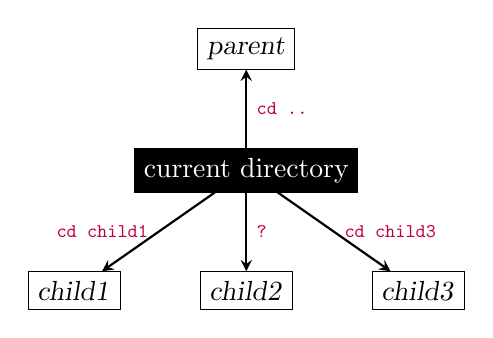
\begin{tikzpicture}[remember picture]
    \tikzstyle{dir} = [
      rectangle,
      draw,
      anchor=north,
      align=center,
    ]
    \tikzstyle{arrow} = [
      thick,
      ->,
      >=stealth,
      draw=black,
    ]
    
    \newcommand{\padding}[0]{1cm}
    \newcommand{\concretecommand}[2]{node[midway,#1] {\scalebox{0.7}{\texttt{\textcolor{purple}{#2}}}}}
    
    \coordinate (origo) at (0,0);
    
    \node[dir,fill=black,text=white] (wd) at (origo) {current directory};
    \node[dir,anchor=south] (parent) at ([yshift=\padding] wd.north) {\textsl{parent}};
    \node[dir] (childII) at ([yshift=-\padding] wd.south) {\textsl{child2}};
    \node[dir,anchor=east] (childI) at ([xshift=-\padding] childII.west) {\textsl{child1}};
    \node[dir,anchor=west] (childIII) at ([xshift=\padding] childII.east) {\textsl{child3}};
    
    \draw[arrow] (wd)--(parent) node[midway,right] {\scalebox{0.7}{\texttt{\textcolor{purple}{cd ..}}}};
    \draw[arrow] (wd)--(childI)  node[midway,left] {\scalebox{0.7}{\texttt{\textcolor{purple}{cd child1}}}};
    \draw[arrow] (wd)--(childII)  node[midway,right] {\scalebox{0.7}{\texttt{\textcolor{purple}{?}}}};
    \draw[arrow] (wd)--(childIII)  node[midway,right] {\scalebox{0.7}{\texttt{\textcolor{purple}{cd child3}}}};
  \end{tikzpicture}
\end{center}

  \caption{Navigating the filesystem.}
  \label{fig:bg:processes:navigation}
\end{figure}

\subsection{Working with Files}

Files are stored in a \idx{filesystem}{Filesystem} that is usually persisted on a disk. This works out very well when you \idx{reboot}{Reboot} your computer and see that your data is still there. That would not have been the case had the files been stored in \idx{main memory}{Memory!Main}. However, the computer can only work with data in main memory, so in order to do something with the contents of those files, they will have to be read into memory. And if you want the result of what you end up doing with them to survive a reboot, then you need to store it on the disk again.

\subsubsection{Copying Files}

% what does it mean to copy a file?

% explain it

\begin{figure}[tbp]
  \begin{center}
  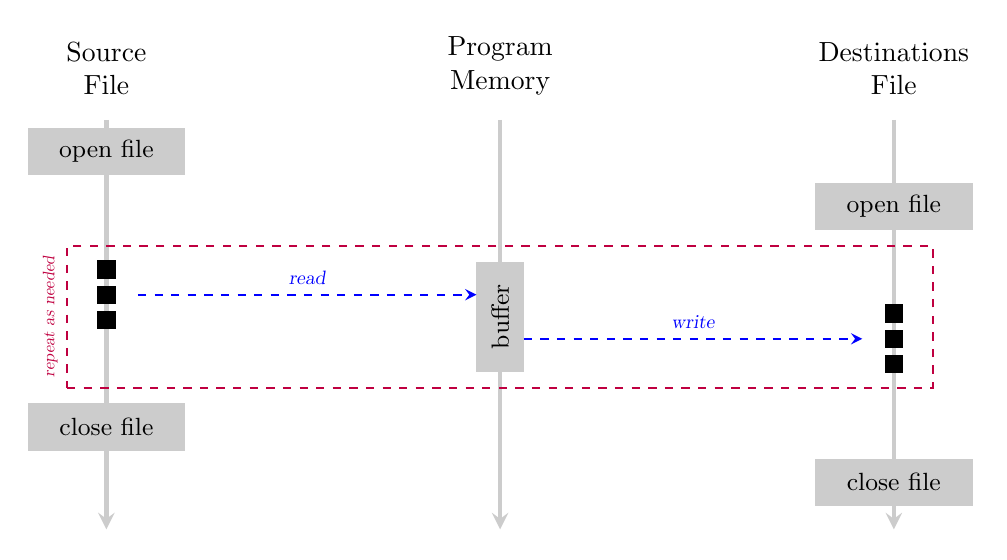
\begin{tikzpicture}[remember picture]
    \tikzstyle{title} = [
      anchor=south,
      align=center,
    ]
    \tikzstyle{arrow} = [
      thick,
      ->,
      >=stealth,
      draw=black,
    ]
    \tikzstyle{fileline}=[
      arrow,
      ultra thick,
      draw=black!20,
    ]
    \tikzstyle{fd} = [
      anchor=center,
      align=center,
      fill=black!20,
      minimum width=2cm,
      minimum height=0.6cm,
    ]
    \tikzstyle{data} = [
      anchor=center,
      fill=black,
      minimum width=1.5mm,
      minimum height=1.5mm,
    ]
    
    \newcommand{\shiftdistance}[0]{5cm}
    \newcommand{\figheight}[0]{5.2cm}
    
    \coordinate (memAnchor) at (0,-1cm);
    \coordinate (srcAnchor) at ([xshift=-\shiftdistance, yshift=0] memAnchor);
    \coordinate (dstAnchor) at ([xshift= \shiftdistance, yshift=0] memAnchor);
    
    % src line
    {
      \node[title] (srcTitle) at ([yshift=2mm] srcAnchor) {Source\\File};
      \draw[fileline] (srcAnchor) -- ([yshift=-\figheight] srcAnchor);
    }
    
    % dst line
    {
      \node[title] (dstTitle) at ([yshift=2mm] dstAnchor) {Destinations\\File};
      \draw[fileline] (dstAnchor) -- ([yshift=-\figheight] dstAnchor);
    }
    
    % mem line
    {
      \node[title] (memTitle) at ([yshift=2mm] memAnchor) {Program\\Memory};
      \draw[fileline] (memAnchor) -- ([yshift=-\figheight] memAnchor);
    }
    
    % open(src)
    {
      \node[fd] (srcOpen) at ([yshift=-4mm] srcAnchor) {\small{open file}};
    }
    
    % open(dst)
    {
      \node[fd] (dstOpen) at ([yshift=-11mm] dstAnchor) {\small{open file}};
    }
    
    % buffer
    {
      \node[fd, minimum width=0.6cm, minimum height=1.4cm] (buffer) at ([yshift=-25mm] memAnchor) {\rotatebox{90}{\small{buffer}}};
    }
    
    % read
    {
      \node[data] (srcDataI)   at ([yshift=-19mm] srcAnchor) {};
      \node[data] (srcDataII)  at ([yshift=-3.2mm] srcDataI) {};
      \node[data] (srcDataIII) at ([yshift=-3.2mm] srcDataII) {};
      
      \draw[arrow, dashed, draw=blue]
        ([xshift=4mm] srcDataII.center)--([xshift=\shiftdistance-0.3cm] srcDataII.center)
        node[midway,sloped,above]
        {\scalebox{0.7}{\textsl{\textcolor{blue}{read}}}};
    }
    
    % write
    {
      \node[data] (dstDataIII) at ([yshift=-31mm] dstAnchor) {};
      \node[data] (dstDataII)  at ([yshift=3.2mm] dstDataIII) {};
      \node[data] (dstDataI)   at ([yshift=3.2mm] dstDataII) {};
      
      \draw[arrow, dashed, draw=blue]
        ([xshift=-\shiftdistance+0.3cm] dstDataII.center)--([xshift=-4mm] dstDataII.center)
        node[midway,sloped,above]
        {\scalebox{0.7}{\textsl{\textcolor{blue}{write}}}};
    }
    
    % repetition
    {
      \node[rectangle, thick, dashed, draw=purple, anchor=center, minimum width=2*\shiftdistance+10mm, minimum height=1.8cm] (repetition) at ([yshift=-25mm] memAnchor) {};
      \node[] (repetitionLabel) at ([xshift=-2mm] repetition.west) {\rotatebox{90}{\scalebox{0.60}{\textsl{\textcolor{purple}{repeat as needed}}}}};
    }
    
    % close(src)
    {
      \node[fd] (srcOpen) at ([yshift=-39mm] srcAnchor) {\small{close file}};
    }
    
    % close(dst)
    {
      \node[fd] (dstOpen) at ([yshift=-46mm] dstAnchor) {\small{close file}};
    }
  \end{tikzpicture}
\end{center}

  \caption{The process of copying a file.}
  \label{fig:bg:processes:copy}
\end{figure}

\subsubsection{Editing Files}

% what does it mean to edit a file?
When we edit a file, we change the contents of that file. If we add something to the beginning, then the old contents needs to be shifted forward to make space for the new material. If we add something at the end, then some material can be easily added. If the modification happens anywhere in between then part of the original contents needs to be moved. Doing these operations on disk would be highly ineffective. So, in reality it happens in the computers memory and the saving to disk is initiated by either a human intervention or something like a \idx{timeout}{Timeout}.

% explain it
Figure \ref{fig:bg:processes:edit} illustrates how a typical \idx{text editor}{Text editor} will work with a file. First the file is \idx{opened}{File!Opening}. Then, the contents of the file is read and written to \idx{primary memory}{Memory!Primary}. The user may then manipulate the in-memory representation through some user interface, and saved the modified buffer (memory representation) to disk. Finally, the program will \idx{close}{File!Closing} the file.

\begin{figure}[tbp]
  \begin{center}
  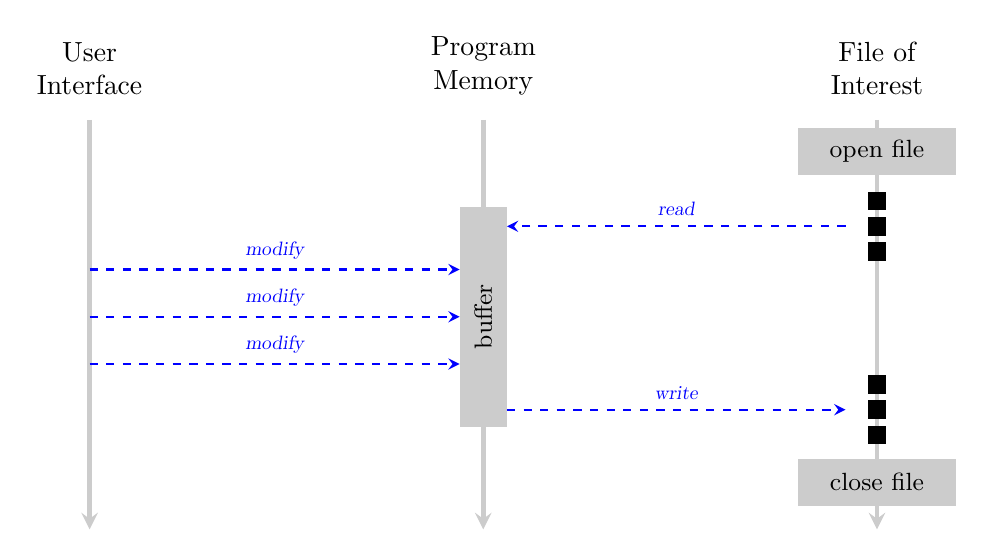
\begin{tikzpicture}[remember picture]
    \tikzstyle{title} = [
      anchor=south,
      align=center,
    ]
    \tikzstyle{arrow} = [
      thick,
      ->,
      >=stealth,
      draw=black,
    ]
    \tikzstyle{fileline}=[
      arrow,
      ultra thick,
      draw=black!20,
    ]
    \tikzstyle{fd} = [
      anchor=center,
      align=center,
      fill=black!20,
      minimum width=2cm,
      minimum height=0.6cm,
    ]
    \tikzstyle{data} = [
      anchor=center,
      fill=black,
      minimum width=1.5mm,
      minimum height=1.5mm,
    ]
    
    \newcommand{\shiftdistance}[0]{5cm}
    \newcommand{\moddistance}[0]{6mm}
    \newcommand{\figheight}[0]{5.2cm}
    
    \coordinate (memAnchor) at (0,-1cm);
    \coordinate (userAnchor) at ([xshift=-\shiftdistance, yshift=0] memAnchor);
    \coordinate (fileAnchor) at ([xshift= \shiftdistance, yshift=0] memAnchor);
    
    % user line
    {
      \node[title] (userTitle) at ([yshift=2mm] userAnchor) {User\\Interface};
      \draw[fileline] (userAnchor) -- ([yshift=-\figheight] userAnchor);
    }
    
    % file line
    {
      \node[title] (fileTitle) at ([yshift=2mm] fileAnchor) {File of\\Interest};
      \draw[fileline] (fileAnchor) -- ([yshift=-\figheight] fileAnchor);
    }
    
    % mem line
    {
      \node[title] (memTitle) at ([yshift=2mm] memAnchor) {Program\\Memory};
      \draw[fileline] (memAnchor) -- ([yshift=-\figheight] memAnchor);
    }
    
    % open(file)
    {
      \node[fd] (fileOpen) at ([yshift=-4mm] fileAnchor) {\small{open file}};
    }
    
    % buffer
    {
      \node[fd, minimum width=0.6cm, minimum height=2.8cm] (buffer) at ([yshift=-25mm] memAnchor) {\rotatebox{90}{\small{buffer}}};
    }
    
    % read
    {
      \node[data, anchor=north] (dataI)   at ([yshift=-2mm] fileOpen.south) {};
      \node[data] (dataII)  at ([yshift=-3.2mm] dataI) {};
      \node[data] (dataIII) at ([yshift=-3.2mm] dataII) {};
      
      \draw[arrow, dashed, draw=blue]
        ([xshift=-4mm] dataII.center)--([xshift=-\shiftdistance+0.3cm] dataII.center)
        node[midway,sloped,above]
        {\scalebox{0.7}{\textsl{\textcolor{blue}{read}}}};
    }
    
    % modify 1
    {
      \draw[arrow, dashed, draw=blue]
        ([xshift=-\shiftdistance, yshift=\moddistance] buffer.center)--([xshift=-0.3cm, yshift=\moddistance] buffer.center)
        node[midway,sloped,above]
        {\scalebox{0.7}{\textsl{\textcolor{blue}{modify}}}};
    }
    
    % modify 2
    {
      \draw[arrow, dashed, draw=blue]
        ([xshift=-\shiftdistance, yshift=0mm] buffer.center)--([xshift=-0.3cm, yshift=0mm] buffer.center)
        node[midway,sloped,above]
        {\scalebox{0.7}{\textsl{\textcolor{blue}{modify}}}};
    }
    
    % modify 3
    {
      \draw[arrow, dashed, draw=blue]
        ([xshift=-\shiftdistance, yshift=-\moddistance] buffer.center)--([xshift=-0.3cm, yshift=-\moddistance] buffer.center)
        node[midway,sloped,above]
        {\scalebox{0.7}{\textsl{\textcolor{blue}{modify}}}};
    }
    
    % write
    {
      \node[data] (dstDataIII) at ([yshift=-40mm] fileAnchor) {};
      \node[data] (dstDataII)  at ([yshift=3.2mm] dstDataIII) {};
      \node[data] (dstDataI)   at ([yshift=3.2mm] dstDataII) {};
      
      \draw[arrow, dashed, draw=blue]
        ([xshift=-\shiftdistance+0.3cm] dstDataII.center)--([xshift=-4mm] dstDataII.center)
        node[midway,sloped,above]
        {\scalebox{0.7}{\textsl{\textcolor{blue}{write}}}};
    }
    
    % close(file)
    {
      \node[fd] (fileClose) at ([yshift=-46mm] fileAnchor) {\small{close file}};
    }
  \end{tikzpicture}
\end{center}

  \caption{The process of editing a file.}
  \label{fig:bg:processes:edit}
\end{figure}


\section{File Formats}

% intro

\begin{figure}[tbp]
  \section{File Formats}

% intro

\begin{figure}[tbp]
  \input{figs/background_fileformats.tex}
  \caption{The relationship between programs, file formats and functions.}
  \label{fig:bg:fileformats}
\end{figure}

  \caption{The relationship between programs, file formats and functions.}
  \label{fig:bg:fileformats}
\end{figure}

\section{Programming Languages}
\label{sec:lang}

\begin{inspiration}{\idx{Larry Wall}{Wall, Larry}\cite{progLangJurassicPark}}
  \quoted{It might seem easy enough, but computer language design is just like a stroll in the park. Jurassic Park, that is.}
\end{inspiration}

% intro
In order to build a program, we describe \textsl{how} that program should work or \textsl{what} it should do. This is done according to the formalized rules of a \defi{programming language}{Programming language}. Most such languages will have high-level abstractions (compared the the assembly instructions known to the machine). They are designed in such a way that a human can reason about them. Those descriptions are stored in files and referred to as \idx{source code}{Source code}. Later on, that source code in converted into instructions and executed.

% different languages and categorization
There are many programming languages to pick from, and they each have strong and weak points. When faced with a particular problem it is important to pick a language that have relevant strong points and acceptable weak points. Many properties can be used to classify these languages. Figure \ref{fig:background:lang:categorization} focuses on two properties, namely whether there is a separate phase for compiling and whether a garbage collector is employed.

\begin{figure}[tbp]
  \centering

% inspiration: https://tex.stackexchange.com/questions/309425/how-is-it-possible-to-make-a-magic-quadrant
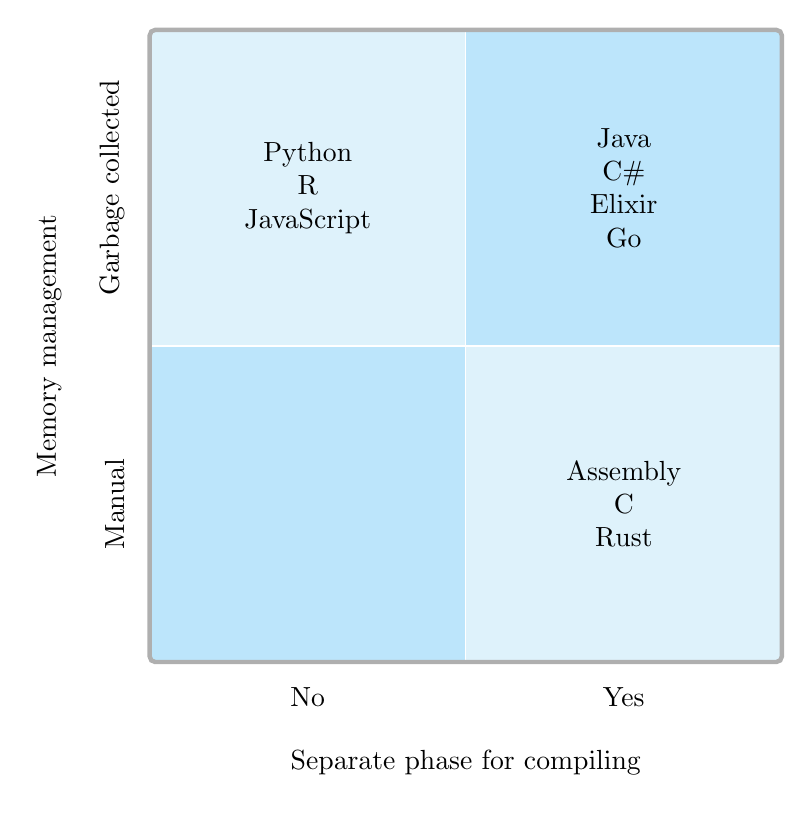
\begin{tikzpicture}[squares/.style={align=center, text width=3cm, minimum width=4cm, minimum height=4cm}]
  \node[squares,fill=lightblue] (A) at (0,0) {Python\\R\\JavaScript};
  \node[squares,fill=darkblue,anchor=west] (B) at (A.east) {Java\\\csharp\\Elixir\\Go};
  \node[squares,fill=darkblue,anchor=north] (C) at (A.south){};
  \node[squares,fill=lightblue,anchor=north] (D) at (B.south) {Assembly\\C\\Rust};
  \node[inner sep=0pt,draw=grey,ultra thick,rounded corners=2pt,fit=(A)(B)(C)(D)] {}; 
  
  \node[anchor=east,xshift=-2mm] at (A.west) {\rotatebox{90}{Garbage collected}};
  \node[anchor=east,xshift=-1cm,align=right] at (A.south west) {\rotatebox{90}{Memory management}};
  \node[anchor=east,xshift=-2mm] at (C.west) {\rotatebox{90}{Manual}};
  \node[anchor=north,yshift=-2mm] at (C.south) {No};
  \node[anchor=north,yshift=-1cm] at (C.south east) {Separate phase for compiling};
  \node[anchor=north,yshift=-2mm] at (D.south) {Yes};
\end{tikzpicture}

  \caption{Categorization of programming languages.}
  \label{fig:background:lang:categorization}
\end{figure}

% separate compilation phase
As programming languages are designed for humans to write, and the machine only understands assembly instructions, something has to \idx{compile}{Compilation} the language into these instructions. Technically, this is always a separate step, but that can be more or less obvious to the user. Some compilers will give the option of compiling the code when you try to execute the code. So, the boundary is a bit fluid. Here, we are using whether the compiled code is stored on disk after compilation as the arbiter. Languages where this is not the case are often used for tying together workflows involving many processes and files. These are called \idx{scripting languages}{Programming language!Scripting}. \csharp\ is a compiled language and not a script language (even though Microsoft likes to talk about \csharp\ scripts).

% garbage collection
Throughout the lifecycle of a process, it will need temporary chunks of memory to do its work. These chunks can be of different size and the need for this can come at varying frequency. We say that the kernel \idx{allocates}{Memory!Allocation} memory to the process on demand. This ensures that the process has exclusive access to this piece of memory and thus that no other process can interfere with its business\footnote{In reality this can be be avoided through shared segments of memory, but that is a topic way too advanced for this book.}. Once the process is done with this piece of memory it is \idx{deallocated}{Memory!Deallocation} (or \idx{freed}{Memory!Freeing}) so that it can be reclaimed by the kernel and put to use later on. This process of allocation and deallocation is manual in some languages and automatic in others. When automatic, a \idx{garbage collector}{Garbage collector} component is compiled into the running code. It essentially scans all allocations and deallocate those that are no longer in use. Again, there are pros and cons with each solution. \csharp\ is a garbage collected language.

\subsection{Parsing}

% file content
The contents of a file is a sequence of \defi{bytes}{Byte}, i.e., units that each have one of 256 possible values. When we write text, these bytes are interpreted as characters and the programs we use to open such files choose to draw each character to the right of the previous one. At \idx{line breaks}{Line break} -- represented by a specific sequence of characters -- the horizontal position is moved all the way to the left and the vertical position is moved one line height down. Some programs break lines that are too wide for your screen. But that's about it. Such a text file does not contain any information about font or text size. If you want to store such information, you have to introduce a \idx{file format}{File format} that \idx{encodes}{Encoding} such information by special \idx{markup}{Markup}. But this is not relevant for files that contain code.

% human interpretation
Files containing code are raw \idx{text files}{Text file}: A sequence of characters with line breaks. As programmers, we manipulate these files through a \idx{text editor}{Text editor}, which most often -- in addition to displaying these characters -- chooses to \idx{color}{Color}-code selected subsequences to make the text more readable for \idx{humans}{Human}. However, these colors represent an \textsl{interpretation} that the tool uses to enrich the code that is actually stored. Modifying the file and saving it will not cause the interpretation to be stored, but only the underlying code. Similarly, there are some such editors that number the lines, highlight a current line, and mark matching parentheses.

% machine interpretation
The text these files contain is called \textsl{\idx{program code}{Program code}} (or simply \textsl{code}), and we change it in much the same way as we change a written report. But when we ask the computer to \idx{execute}{Execute} our program code, it sees the file in a different way. The content is of course the same, but the \textsl{interpretation} is different: Based on some rules, the computer builds a \idx{tree}{Tree} structure of the code. This process is called \idx{parsing}{Parsing} the source code.

%% TODO: tree structure

%\subsubsection{Rules}

%% https://homepage.ruhr-uni-bochum.de/jan.holthuis/posts/using-the-latex-rail-package

%\subsubsection{Parse Trees}

%% https://tex.stackexchange.com/questions/111564/create-a-syntax-tree-with-latex

\section{The Machine}
\label{sec:machine}

\subsection{History}

% Antikythera mechanism https://en.wikipedia.org/wiki/Antikythera_mechanism

% Jacquard machine https://en.wikipedia.org/wiki/Jacquard_machine

% Difference Engine https://en.wikipedia.org/wiki/Difference_engine

% Mutual Exclusion https://en.wikipedia.org/wiki/Mutual_exclusion

% C https://en.wikipedia.org/wiki/C_(programming_language)

% Taming of the Alpaca

\subsection{Overview}

% description of computer: model description as data flow (input, memory, processor, load instruction, registers, operator instructions, ALU, store instruction, memory, output)
Figure \ref{fig:machine:computer} shows the model of a computer that we will rely on. Input (e.g, from keyboard) ends up in the computers \idx{main memory}{Memory!Main}. The processor, as the name implies, \textsl{processes} \idx{instructions}{Instruction}. Each \idx{processor architecture}{Architecture!Processor} or type supports some instruction repertoire. In that repertoire you will find instructions for load values from main memory into registers. \idx{Registers}{Register} are named values that the processor can instructions can access directly. Other instructions performs operations on registers (e.g., for adding two values). Such instructions are processed by something called an arithmetic logic unit (or \idx{ALU}{ALU} in daily speech). Yet other instructions can store the value of a register to main memory. We also say that we \say{write to memory}. Storing values to certain portions of memory yields an output. For instance, some computers have a \idx{frame buffer}{Frame buffer} in main memory that defines what ends up on your screen. Writing to that part of the memory will affect what you see on your screen.

\begin{figure}[tbp]
  \begin{center}
  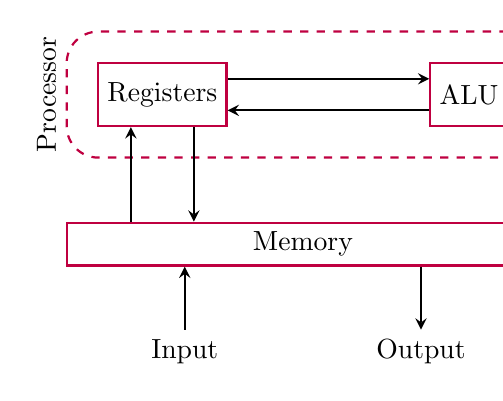
\begin{tikzpicture}[remember picture]
    \newcommand{\spacing}[0]{ 8mm }
    \tikzstyle{edge}  = [thick,>=stealth,draw=black]
    \tikzstyle{dedge} = [thick,->,>=stealth,draw=black]
    \tikzstyle{node}=[
      overlay,
      rectangle,
      draw=purple,
      anchor=center,
      thick,
    ]
    
    \node[node,minimum height=2*\spacing,minimum width=6cm,rounded corners=4mm,dashed] (processor) at (0,0) {};
    \node[anchor=east] (processor_label) at
      (processor.west)
      {\rotatebox{90}{Processor}};
    \node[node,anchor=north west,minimum height=\spacing] (registers) at
      ([xshift=0.5*\spacing,yshift=-0.5*\spacing]processor.north west)
      {Registers};
    \node[node,anchor=north east,minimum height=\spacing] (alu) at
      ([xshift=-0.5*\spacing,yshift=-0.5*\spacing]processor.north east)
      {ALU};
    \node[node,anchor=north,minimum width=6cm] (memory) at
      ([yshift=-\spacing]processor.south)
      {Memory};
    \node[anchor=north] (input) at
      ([xshift=-1.5cm,yshift=-\spacing]memory.south)
      {Input};
    \node[anchor=north] (output) at
      ([xshift=1.5cm,yshift=-\spacing]memory.south)
      {Output};
    
    % register <-> alu
    \draw[dedge] ([yshift= 2mm]registers.east)
               --([yshift= 2mm]alu.west);
    \draw[dedge] ([yshift=-2mm]alu.west)
               --([yshift=-2mm]registers.east);
    
    % register <-> memory
    \draw[dedge] ([xshift=-4mm,yshift=-1.5*\spacing]registers.south)
               --([xshift=-4mm]                     registers.south);
    \draw[dedge] ([xshift= 4mm]                     registers.south)
               --([xshift= 4mm,yshift=-1.5*\spacing]registers.south);
%    \draw[dedge] ()--();
    
    % memory <-> i/o
    \draw[dedge] (                 input.north)
               --([yshift=\spacing]input.north);
    \draw[dedge] ([yshift=\spacing]output.north)
               --(                 output.north);
  \end{tikzpicture}
\end{center}

  \caption{Model of computer.}
  \label{fig:machine:computer}
\end{figure}

% focus on RISC-V
There are many different \idx{processor architectures}{Architecture!Processor}. Popular ones include \idx{AMD64}{AMD64}, \idx{ARM}{ARM} and \idx{RISC-V}{RISC-V}. In this book, we will look into the integer side of the 32-bit RISC-V architecture (aka the \idx{RV32I}{RV32I} instruction set). This is a simple instruction set and architecture, and the model of this is transferable to the other processor architectures for the purposes of this book.

\subsection{Memory Model}

\begin{figure}[tbp]
  \begin{center}
  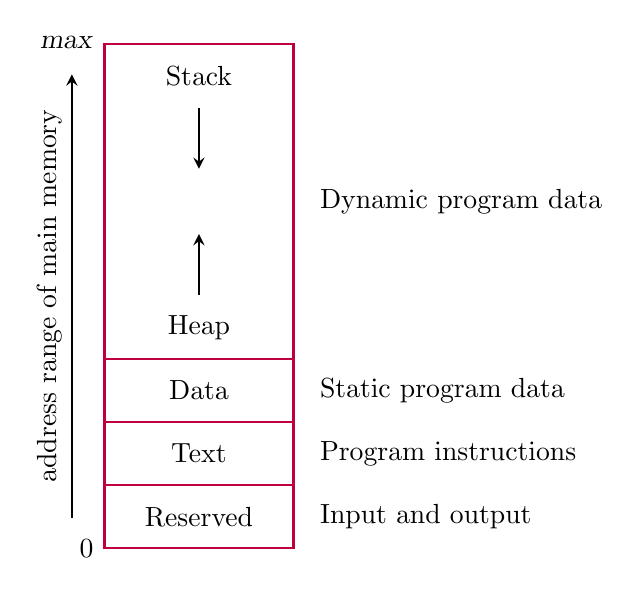
\begin{tikzpicture}[]
    \newcommand{\cellheight}[0]{8mm}
    \newcommand{\cellwidth}[0]{24mm}
    
    \tikzstyle{dedge} = [thick,->,>=stealth,draw=black]
    
    \tikzstyle{cell}=[
      rectangle,
      draw=purple,
      anchor=north,
      thick,
      minimum height=\cellheight,
      minimum width=\cellwidth,
    ]
    \tikzstyle{address}=[
      anchor=east,
    ]
    \tikzstyle{comment}=[
      anchor=west,
    ]
    
    \node[cell,minimum height=5*\cellheight] (dynsegment) at (0, -0*\cellheight) {};
    \node[cell,draw=none] (stacksegment) at (0, -0*\cellheight) {Stack};
    \node[cell,draw=none] (dotssegment) at (0, -2*\cellheight) {};
    \node[cell,draw=none] (heapsegment) at (0, -4*\cellheight) {Heap};
    \node[cell] (datasegment) at (0, -5*\cellheight) {Data};
    \node[cell] (textsegment) at (0, -6*\cellheight) {Text};
    \node[cell] (reservedsegment) at (0, -7*\cellheight) {Reserved};
    
    \node[address] () at (reservedsegment.south west) {$0$};
    \node[address] () at (dynsegment.north west) {\textsl{max}};
    
    \node[comment] () at ([xshift=2mm]dynsegment.east) {Dynamic program data};
    \node[comment] () at ([xshift=2mm]datasegment.east) {Static program data};
    \node[comment] () at ([xshift=2mm]textsegment.east) {Program instructions};
    \node[comment] () at ([xshift=2mm]reservedsegment.east) {Input and output};
    
    \draw[dedge] (stacksegment) -- (dotssegment);
    \draw[dedge] (heapsegment) -- (dotssegment);
    
    \draw[dedge] ([xshift=-4mm,yshift= 4mm]reservedsegment.south west)
              -- ([xshift=-4mm,yshift=-4mm]dynsegment.north west)
              node[midway,sloped,above] {address range of main memory}
    ;
  \end{tikzpicture}
\end{center}

  \caption{Memory model.}
  \label{fig:machine:memory}
\end{figure}

\subsection{Registers}

% how many, special roles?

% figure: caller saved, callee saved
\begin{figure}[tbp]
  \begin{center}
  \begin{tabular}{|l|l|l|c|}
    \hline
    Register & ABI Name & Description & Saver \\
    \hline
    \regname{x0} & \regname{zero} & Hard-wired to zero & --- \\
    \regname{x1} & \regname{ra} & Return address & caller \\
    \regname{x2} & \regname{sp} & Stack pointer & callee \\
    \regname{x3} & \regname{gp} & Global pointer & --- \\
    \regname{x4} & \regname{tp} & Thread pointer & --- \\
    \regname{x5} & \regname{t0} & Temporary/alternate link register & caller \\
    \regname{x6-7} & \regname{t1-2} & Temporaries & caller \\
    \regname{x8} & \regname{s0/fp} & Saved register/frame pointer & callee \\
    \regname{x9} & \regname{s1} & Saved register & callee \\
    \regname{x10-11} & \regname{a0-1} & Function arguments/return values & caller \\
    \regname{x12-17} & \regname{a2-7} & Function arguments & caller \\
    \regname{x18-27} & \regname{s2-11} & Saved registers & callee \\
    \regname{x28-31} & \regname{t3-6} & Temporaries & caller \\
    \hline
  \end{tabular}
\end{center}

  \caption{Register overview.}
  \label{fig:machine:regs}
\end{figure}

%TODO: we need an introduction to branches and loops in order to talk aller/callee saved registers. Where should it be placed?

\subsection{Instructions}

% intro
The instruction repertoire of the majority of instruction sets is fairly large.

%TODO: where to introduce instruction sets

\subsubsection{Memory Access}

% access model: most program data is in main memory, we can only operate on registers and we have a limited number of these, (we need a way of loading data from main memory into registers so that we can work on it, and then store the results back into main memory to make space -- in the registers -- for more useful work)
The processor can only operate on registers, but has a very limited number of them. For 32 bit RISC-V, there are 32 of them. That is only enough for the smallest of programs, and nothing that can be written in \csharp. Instead, most program data resides in main memory. This means that we need a way of loading data from main memory into registers so that we can work on it, and then another way of storing the results back into main memory to make (register) space for other data. This way, we can continue to do useful work.

% enumerate: load and store instructions
We have a number of instructions for loading and storing data. In this description, we only care about those that operates on \textsl{words}. A \defi{word}{Word} is the type of integer that matches the size that the processor is optimized to work on. In our case, it is a 32 bit integer.
\begin{itemize}
  \item \texttt{LW} (\say{load word}) This loads a word from an address in main memory into a named register in the processor.
  \item \texttt{SW} (\say{store word}) Stores the value of a named register in the processor to an address in main memory.
\end{itemize}
These addresses are the sum of the value of a register, and a 12-bit integer that is encoded in (read: part of) the instruction itself. That last part acts as a static offset to the value in the register.

\subsubsection{Arithmetic Operations}

% intro: what is?, operation interface (1-2 inputs, 1 output), examples

% register and immediate variants

% floats: in this book we only cover integers, similar instructions exist for floats

\subsubsection{Choice}

% source: https://docs.openhwgroup.org/projects/cva6-user-manual/01_cva6_user/RISCV_Instructions_RV32I.html#control-transfer-instructions

Unconditional branch instructions:
\begin{itemize}
  \item \texttt{J} (\say{jump}) Jump to a specific memory address.
  \item \texttt{JAL} (\say{jump and link}) Jump to a specific memory address, and \textsl{link}.
\end{itemize}

Conditional branch instructions (no link):
\begin{itemize}
  \item \texttt{BNE} (\say{branch not equal}) Jump to a specific memory address if two register have different values. Otherwise continue.
  \item \texttt{BLT} (\say{branch lest than}) Jump to a specific memory address if one register has a value that is less than that of another one. Otherwise continue.
\end{itemize}

\subsubsection{Instruction Format Types}


\subsection{Big Picture}

% intro
The components that of the machine that we have covered can be put together around the central processing unit (i.e., the \idx{CPU}{CPU}). An implementation of a primitive RISC-V processor is illustrated in figure \ref{fig:machine:riscv}. In reality, it is much more complicated, and RISC-V is a simple \idx{processor architecture}{Architecture!Processor}. Lets briefly go through what is going on in this figure.

\begin{figure}[tbp]
  \centering

\rotatebox{90}{
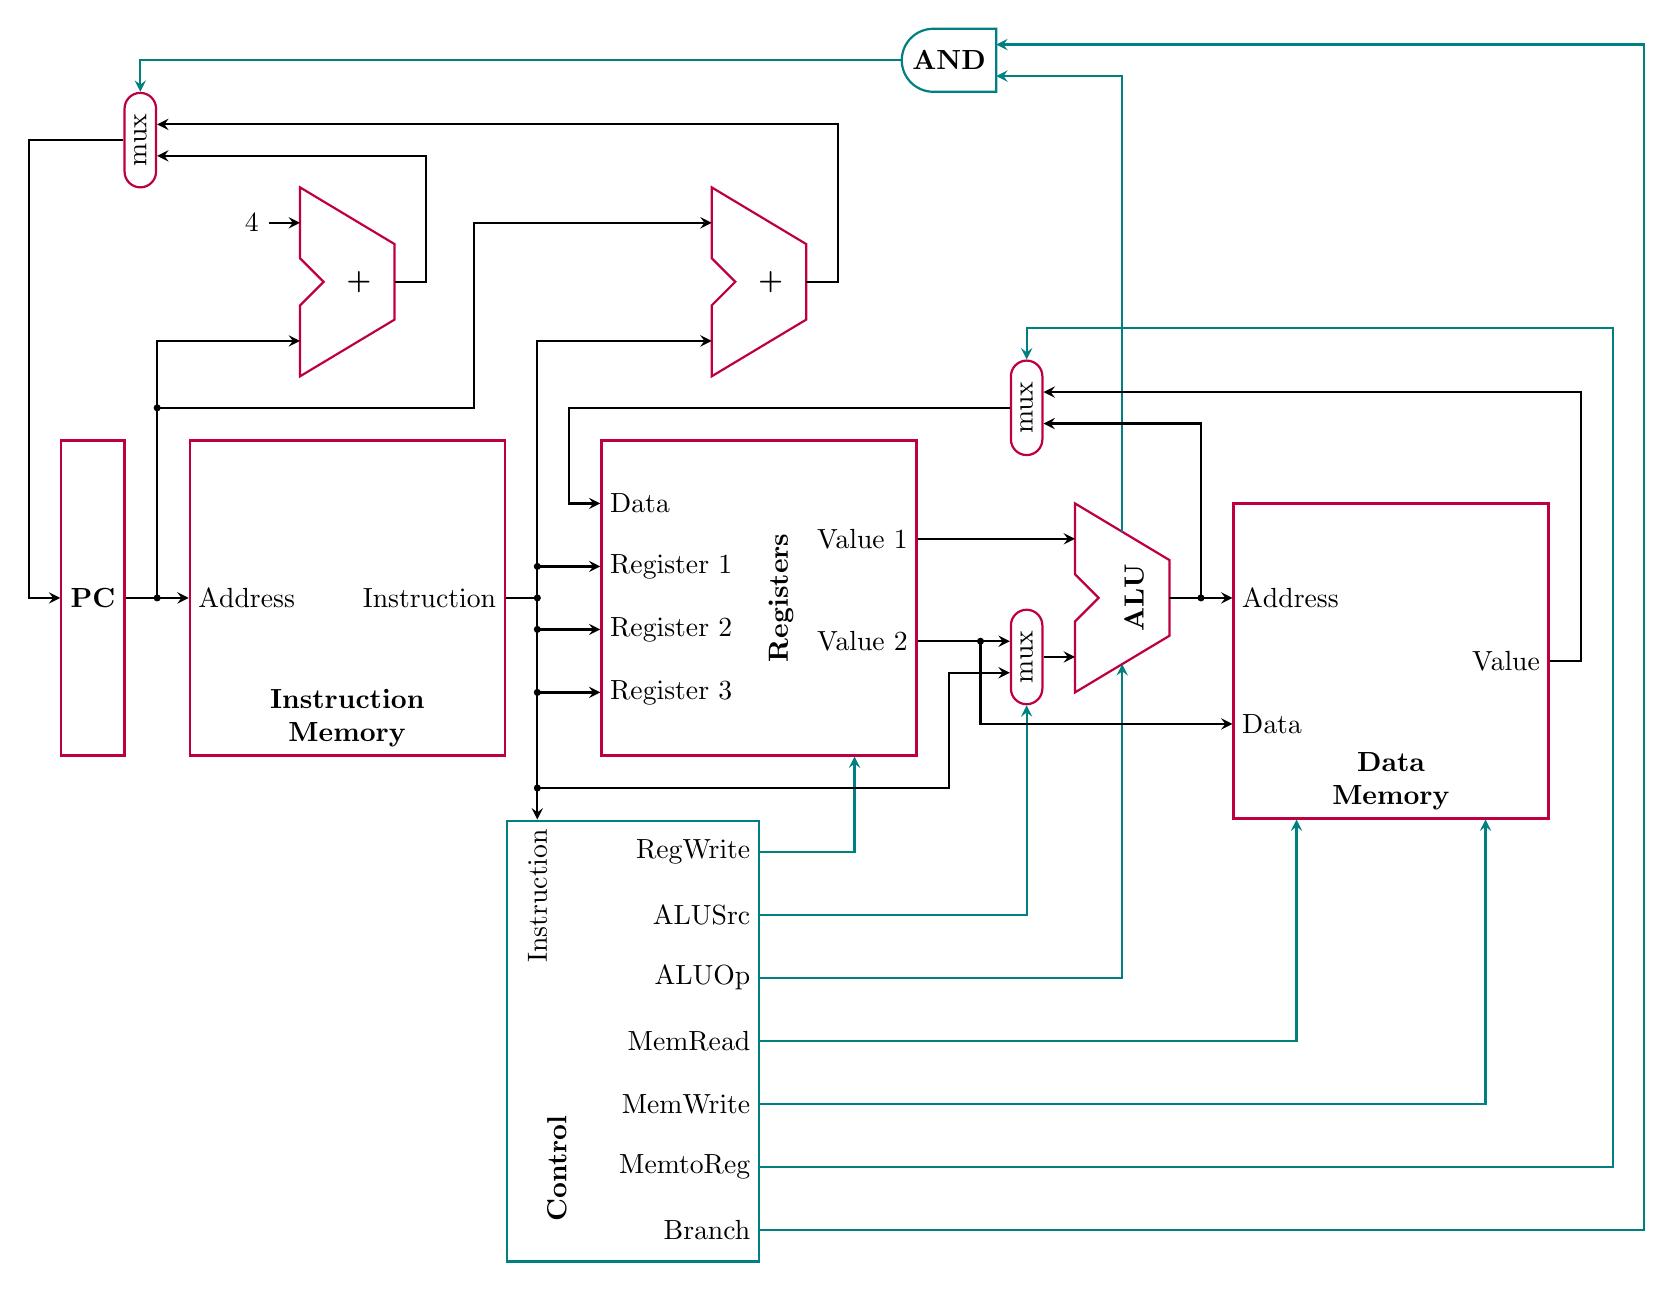
\begin{tikzpicture}[]
  \newcommand{\Xpc}[0]{ 0mm }
  \newcommand{\Xim}[0]{ 32mm }
  \newcommand{\Xreg}[0]{ 56mm }
  \newcommand{\Xloadmux}[0]{ 65mm }
  \newcommand{\Xdm}[0]{ 80mm }
  \newcommand{\Ycenter}[0]{ 8mm }
  
  \newcommand{\spacing}[0]{ 4mm }
  \newcommand{\lineheight}[0]{ 8mm }
  
  \newcommand{\andheight}[0]{ 8mm }
  \newcommand{\andwidth}[0]{ (1.5*\andheight) }
  \newcommand{\muxwidth}[0]{ 4mm }
  \newcommand{\muxheight}[0]{ (\spacing+2*\muxwidth) }
  \newcommand{\muxinputoffset}[0]{ (\spacing/2) }
  \newcommand{\aluheight}[0]{ 24mm }
  \newcommand{\aluwidth}[0]{ 12mm }
  \newcommand{\aluindent}[0]{ 3mm }
  \newcommand{\aluinputoffset}[0]{ (\aluheight/4+\aluindent/2) }
  
  \tikzstyle{edge}  = [thick,>=stealth,draw=black]
  \tikzstyle{dedge} = [thick,->,>=stealth,draw=black]
  \tikzstyle{control} = [draw=teal]
  \tikzstyle{block}=[
    rectangle,
    draw=purple,
    anchor=center,
    align=center,
    thick,
  ]
  \tikzstyle{mux}=[
    rectangle,
    draw=purple,
    anchor=center,
    align=center,
    rounded corners=\muxwidth/2,
    minimum width=\muxwidth,
    minimum height=\muxheight,
    thick,
  ]
  \tikzstyle{point}=[
    circle,
    fill=black,
    anchor=center,
    minimum size=0.9mm,
    inner sep=0pt,
    thick,
  ]
  
  % #1: prefix
  % #2: position
  \newcommand{\buildProgramCounterBlock}[2]{
    \node[
      block,
      anchor=west,
      minimum height=40mm,
    ] (#1) at (#2) {\textbf{PC}};
    
    \coordinate (#1 in)  at (#1.west);
    \coordinate (#1 out) at (#1.east);
  }
  
  % #1: prefix
  % #2: position
  \newcommand{\buildInstructionMemoryBlock}[2]{
    \node[
      block,
      anchor=west,
      minimum width=40mm,
      minimum height=40mm,
    ] (#1) at (#2) {};
    \node[anchor=south,align=center] () at (#1.south) {\textbf{Instruction}\\\textbf{Memory}};
    
    \coordinate (#1 addr) at ([yshift=0.0*\lineheight]#1.west);
    \coordinate (#1 inst) at ([yshift=0.0*\lineheight]#1.east);
    
    \node[anchor=west] () at (#1 addr) {Address};
    \node[anchor=east] () at (#1 inst) {Instruction};
  }
  
  % #1: prefix
  % #2: position
  \newcommand{\buildRegisterBlock}[2]{
    \node[
      block,
      anchor=west,
      minimum width=40mm,
      minimum height=40mm,
    ] (#1) at (#2) {};
    \node[anchor=west] () at (#1.center) {\rotatebox{90}{\textbf{Registers}}};
    
    \coordinate (#1 data)   at ([yshift= 1.5*\lineheight]#1.west);
    \coordinate (#1 regI)   at ([yshift= 0.5*\lineheight]#1.west);
    \coordinate (#1 regII)  at ([yshift=-0.5*\lineheight]#1.west);
    \coordinate (#1 regIII) at ([yshift=-1.5*\lineheight]#1.west);
    \coordinate (#1 valI)   at ([yshift= \aluinputoffset]#1.east);
    \coordinate (#1 valII)  at ([yshift=-\aluinputoffset+\muxinputoffset]#1.east);
    
    \node[anchor=west] () at (#1 data)   {Data};
    \node[anchor=west] () at (#1 regI)   {Register 1};
    \node[anchor=west] () at (#1 regII)  {Register 2};
    \node[anchor=west] () at (#1 regIII) {Register 3};
    \node[anchor=east] () at (#1 valI)   {Value 1};
    \node[anchor=east] () at (#1 valII)  {Value 2};
    
    \coordinate (#1 rw) at ([xshift=-2*\spacing]#1.south east);
  }
  
  % #1: prefix
  % #2: position
  \newcommand{\buildDataMemoryBlock}[2]{
    \node[
      block,
      anchor=west,
      minimum width=40mm,
      minimum height=40mm,
    ] (#1) at (#2) {};
    \node[anchor=south,align=center] () at (#1.south) {\textbf{Data}\\\textbf{Memory}};
    
    \coordinate (#1 addr)  at ([yshift= 1.0*\lineheight]#1.west);
    \coordinate (#1 data)  at ([yshift=-1.0*\lineheight]#1.west);
    \coordinate (#1 value) at ([yshift= 0.0*\lineheight]#1.east);
    
    \node[anchor=west] () at (#1 addr) {Address};
    \node[anchor=west] () at (#1 data) {Data};
    \node[anchor=east] () at (#1 value) {Value};
  }
  
  
  % #1: prefix
  % #2: position
  \newcommand{\buildALU}[3]{
    \coordinate (offset) at (#2);
    
    \draw[
      thick,
      draw=purple,
    ]  ([yshift=\aluheight/2]offset)
    -- ([xshift=\aluwidth,yshift= \aluheight/5]offset)
    -- ([xshift=\aluwidth,yshift=-\aluheight/5]offset)
    -- ([yshift=-\aluheight/2]offset)
    -- ([yshift=-\aluindent]offset)
    -- ([xshift=\aluindent]offset)
    -- ([yshift=\aluindent]offset)
    -- cycle;
    \node[anchor=center,align=center] () at ([xshift=\aluindent+\aluwidth/2-\aluindent/2]offset) {\rotatebox{90}{\textbf{#3}}};
    
    \coordinate (#1 iI)  at ([yshift= \aluinputoffset]offset);
    \coordinate (#1 iII) at ([yshift=-1*\aluinputoffset]offset);
    \coordinate (#1 o)   at ([xshift=\aluwidth]offset);
    \coordinate (#1 c)   at ([xshift=\aluwidth/2,yshift=-(\aluheight/5/2+\aluheight/2/2]offset);
    \coordinate (#1 z)   at ([xshift=\aluwidth/2,yshift= (\aluheight/5/2+\aluheight/2/2]offset);
  }
  
  % #1: prefix
  % #2: position
  \newcommand{\buildAND}[2]{
    \coordinate (offset) at (#2);
    
    \draw[
      thick,
      draw=teal,
    ]  ([xshift=\andwidth/2,yshift= \andheight/2]offset)
    -- ([xshift=\andwidth/2,yshift=-\andheight/2]offset)
    -- ([xshift=-(\andwidth/2-\andheight/2),yshift=-\andheight/2]offset)
    arc [x radius=\andheight/2,y radius=\andheight/2, start angle=270,end angle=90]
    -- cycle;
    \node[anchor=center,align=center] () at (offset) {\rotatebox{0}{\textbf{AND}}};
    
    \coordinate (#1 iI)  at ([xshift=\andwidth/2,yshift= \spacing/2]offset);
    \coordinate (#1 iII) at ([xshift=\andwidth/2,yshift=-\spacing/2]offset);
    \coordinate (#1 o)   at ([xshift=-\andwidth/2]offset);
  }
  
  % #1: prefix
  % #2: position
  \newcommand{\buildControlBlock}[2]{
    \node[
      block,
      anchor=north west,
      minimum width=32mm,
      minimum height=7*\lineheight,
      control,
    ] (#1) at (#2) {};
    \node[anchor=south west] () at ([xshift=\spacing,yshift=\spacing]#1.south west) {\rotatebox{90}{\textbf{Control}}};
    
    \coordinate (#1 Instruction) at ([xshift= 1.0*\spacing]#1.north west);
    \coordinate (#1 RegWrite)    at ([yshift= 3.0*\lineheight]#1.east);
    \coordinate (#1 ALUSrc)      at ([yshift= 2.0*\lineheight]#1.east);
    \coordinate (#1 ALUOp)       at ([yshift= 1.0*\lineheight]#1.east);
    \coordinate (#1 MemRead)     at ([yshift= 0.0*\lineheight]#1.east);
    \coordinate (#1 MemWrite)    at ([yshift=-1.0*\lineheight]#1.east);
    \coordinate (#1 MemtoReg)    at ([yshift=-2.0*\lineheight]#1.east);
    \coordinate (#1 Branch)      at ([yshift=-3.0*\lineheight]#1.east);
    
    \node[anchor=north] () at (#1 Instruction)   {\rotatebox{90}{Instruction}};
    \node[anchor=east] () at (#1 RegWrite) {RegWrite};
    \node[anchor=east] () at (#1 ALUSrc)   {ALUSrc};
    \node[anchor=east] () at (#1 ALUOp)    {ALUOp};
    \node[anchor=east] () at (#1 MemRead)  {MemRead};
    \node[anchor=east] () at (#1 MemWrite) {MemWrite};
    \node[anchor=east] () at (#1 MemtoReg) {MemtoReg};
    \node[anchor=east] () at (#1 Branch)   {Branch};
  }
  
  % program counter
  \buildProgramCounterBlock{pc}{0,0}
  
  % instruction memory
  \buildInstructionMemoryBlock{im}{[xshift=2*\spacing]pc.east}
  
  % instruction increment alu
  \buildALU{alu incr}{[xshift=-\aluwidth/2,yshift=5*\spacing]im.north}{+}
  \node[anchor=east] (inst size) at ([xshift=-\spacing]alu incr iI) {4};
  \draw[dedge] (inst size) -- (alu incr iI);
  
  % registers
  \buildRegisterBlock{reg}{[xshift=3*\spacing]im.east}
  
  % branch alu
  \buildALU{alu branch}{[xshift=-\aluwidth/2,yshift=5*\spacing]reg.north}{+}
  
  % alu
  \buildALU{alu}{[xshift=3*\spacing+\muxwidth+\spacing] reg.east}{ALU}
  
  % immediate mux
  \node[mux,anchor=east] (immediatemux) at ([xshift=-\spacing]alu iII) {\rotatebox{90}{mux}};
  
  % data memory
  \buildDataMemoryBlock{dm}{[xshift=2*\spacing,yshift=-\lineheight]alu o}
  
  % load mux
  \node[mux,anchor=east] (loadmux) at ([xshift=4*\spacing,yshift=\spacing]reg.north east) {\rotatebox{90}{mux}};
  
  % pc mux
  \node[mux,anchor=east] (pcmux) at ([xshift=-\muxwidth,yshift=2*\spacing+\aluheight+\spacing+\muxheight/2-(\muxheight/2-\muxinputoffset)]im.north west) {\rotatebox{90}{mux}};
%  \node[mux,anchor=east] (pcmux) at ([xshift=-\muxwidth,yshift=10*\spacing]im.north west) {\rotatebox{90}{mux}};
  
  % control
  \buildControlBlock{control}{[yshift=-2*\spacing]im.south east}
  
  % control and
  \buildAND{and}{[xshift=\spacing,yshift=\spacing]$(reg.north east)!(pcmux.north)!(reg.south east)$}
  
  % control wiring
  \draw[dedge,control] (control RegWrite) -| (reg rw);
  \draw[dedge,control] (control ALUSrc) -| (immediatemux.south);
  \draw[dedge,control] (control ALUOp) -| (alu c);
  \draw[dedge,control] (alu z) |- (and iII);
  \draw[dedge,control] (and o) -| (pcmux.north);
  \draw[dedge,control] (control MemRead) -| ([xshift=-3*\spacing]dm.south);
  \draw[dedge,control] (control MemWrite) -| ([xshift=3*\spacing]dm.south);
  \draw[dedge,control] (control MemtoReg)
                    -- ([xshift=2*\spacing] $(dm.north east)!(control MemtoReg)!(dm.south east)$)
                    |- ([yshift=\spacing]loadmux.north)
                    -- (loadmux.north);
  \draw[dedge,control] (control Branch)
                    -- ([xshift=3*\spacing] $(dm.north east)!(control Branch)!(dm.south east)$)
                    |- (and iI);
  
  % wiring
  \draw[dedge] (pc out) -- (im addr);
  \draw[dedge] ($(pc out)!0.5!(im addr)$) |- (alu incr iII);
  \draw[dedge] ([xshift=-\spacing,yshift=\spacing]im.north west)
            -- ([xshift=-\spacing,yshift=\spacing]im.north east)
            |- (alu branch iI);
  \draw[dedge] (im inst)
            -- ([xshift=\spacing]im inst)
            |- ([xshift=\spacing,yshift=-\spacing]reg.south east)
            |- ([yshift=-\muxinputoffset]immediatemux.west);
  \draw[dedge] ([xshift=\spacing]im inst)
            |- (alu branch iII);
  \draw[dedge] ([xshift=-2*\spacing]reg regI)   -- (reg regI);
  \draw[dedge] ([xshift=-2*\spacing]reg regII)  -- (reg regII);
  \draw[dedge] ([xshift=-2*\spacing]reg regIII) -- (reg regIII);
  \draw[dedge] ([yshift=1*\spacing]control Instruction) -- (control Instruction);
  \draw[dedge] (reg valI) -- (alu iI);
  \draw[dedge] (reg valII) -- ([yshift=\muxinputoffset] immediatemux.west);
  \draw[dedge] ([xshift=2*\spacing]reg valII) |- (dm data);
  \draw[dedge] (immediatemux) -- (alu iII);
  \draw[dedge] (alu o) -- (dm addr);
  \draw[dedge] ([xshift=\spacing]alu o)
            |- ([yshift=-\muxinputoffset]loadmux.east);
  \draw[dedge] (dm value)
            -- ([xshift=\spacing]dm value)
            |- ([yshift=\muxinputoffset]loadmux.east);
  \draw[dedge] (loadmux.west)
            -- ([xshift=-\spacing,yshift=\spacing]reg.north west)
            |- (reg data);
  \draw[dedge] (alu incr o)
            -- ([xshift=\spacing]alu incr o)
            |- ([yshift=-\muxinputoffset]pcmux.east);
  \draw[dedge] (alu branch o)
            -- ([xshift=\spacing]alu branch o)
            |- ([yshift=\muxinputoffset]pcmux.east);
  \draw[dedge] (pcmux.west)
            -| ([xshift=-\spacing]pc.west)
            |- (pc);
  
  % connection points
  \node[point] () at ([xshift=\spacing]pc.east) {};
  \node[point] () at ([xshift=-\spacing,yshift=\spacing]im.north west) {};
  \node[point] () at ([xshift= 1*\spacing]im inst) {};
  \node[point] () at ([xshift=-2*\spacing]reg regI) {};
  \node[point] () at ([xshift=-2*\spacing]reg regII) {};
  \node[point] () at ([xshift=-2*\spacing]reg regIII) {};
  \node[point] () at ([xshift=2*\spacing]reg valII) {};
  \node[point] () at ([xshift= 1*\spacing]alu o) {};
  \node[point] () at ([yshift=1*\spacing]control Instruction) {};
\end{tikzpicture}
}

  \caption{Primitive model of a RISC-V Processor.}
  \label{fig:machine:riscv}
\end{figure}

% signals: bloacks and arrows, complex blocks, what complex mean, signals (1 or more bits), control and data
The diagram consists of various blocks connected by arrows. These blocks are \idx{complex}{Complex!Block}. That is, they represent a \idx{logical}{Logical} unit but are physically constructed from smaller parts \ldots\ with arrows between them. We call the arrows \idx{signals}{Signal}. They represent a value of one or more bits. One can think of them as how data flows through the processor. Concretely, this is accomplished through \idx{register transfer level}{Register Transfer Level} (RTL) logic and a \idx{clock signal}{Signal!Clock}. But then things get really complicated, and we don't need it that badly.

% data and control plane:
Some of these signals exists to move data around between memory, registers and the implementation of the instructions. These are called \idx{data signals}{Signal!Data}, and we say that these make up the \defi{data plane}{Plane!Data}. This is a cross-cut of the processor through which \say{data flows}. Other signals are \idx{control signals}{Signal!Control}, and they make up the \defi{control plane}{Plane!Control}. That is a different cross-cut that informs the blocks of \textsl{how} they should operate. For instance, the block that executes the instructions is called an ALU. It has a number of generic inputs and a control signal tells it which operation (e.g., an addition or a division) it is supposed to perform on these.

% alu: identifying the component visually, much more complicated block, interface (two data inputs, one control input, one data output, one control output, one control output), perform the operation specified by the control input on the data inputs and output the resulting value on the data output, boolean signal for whether a branch should be taken, two variations (the generic one covered here, a specialized version that can only add and has no control interface)
There are three \idx{ALUs}{ALU} on the diagram. They look a bit like an arrow pointing to the right and are labeled either \say{ALU} or \say{+}. The latter version is a specialized version of the former. The specialized version takes two data inputs and produces a data output. This output is the result of adding the two inputs. The generic version has a control input which tells it which operation to perform. This ALU supports a large number of operations, and will perform the operation specified by the control input on the data inputs and output the resulting value on the data output. For \idx{arithmetic operations}{Operation!Arithmetic}, this is straight forward to imagine: If the control signal specifies a multiplication operation and the data inputs a two and three, then the data output becomes six. Other operations are used to transfer the control flow from one place in \idx{instruction memory}{Memory!Instruction} to another. This can be either conditional (e.g., using the \idx{BNE}{BNE@\texttt{J} instruction} or \idx{BLT}{BLT@\texttt{BLT} instruction} instruction) or unconditional (e.g., using the \idx{J}{J@\texttt{J} instruction} or \idx{JAL}{JAL@\texttt{JAL} instruction} instruction). If a branch operation needs to be executed, the ALU will indicate this using its control output signal.

% and: identifying the component visually, interface (number of inputs, one output), what the output represent
If we follow that control signal from the ALU, we will find a shape labeled \say{AND} that on the input side looks like a rectangle and on the output side it looks like a circle. It is an \idx{AND gate}{Gate!AND}. That is a piece of \idx{digital electronics}{Electronics!Digital} that produces a signal that represents whether all of the inputs are true.

% multiplexers (mux): identifying the component visually, interface (number of inputs, one output, a control), role of control
In the diagram, you will find three \idx{multiplexers}{Multiplexer} (or \idx{mux}{Mux} for short). These are labeled \say{mux}. They each have one outgoing edge, two incoming black edges, and one incoming \textsl{colored} edge. The mux is a selective forwarding mechanism, based on the value of the colored input, it forwards the value on one of the black inputs to its output. For this reason, the colored input is called a \idx{control signal}{Signal!Control}.

\subsubsection{Data Plane}

% pc: a register (something that can hold a value), usually increments in steps of 4, why that is
The execution of an instruction starts at the \idx{program counter}{Program counter} (or PC, for short). It is usually incremented in steps of four as this matches the size of a RISC-V 32-bit instruction. The program counter is a \idx{register}{Register} that holds the address of the next instruction. This address is fed into the program memory block.

% instruction fetch and decode: the next step is to fetch that instruction (at that address) from instruction memory and decode it into its principal components, this usually includes instruction identity and a number of registers or immediate values
The program memory block then \idx{fetches}{Fetching} the instruction that the program counter \idx{points to}{Pointer}. It then decodes it into it principal components. These are the code for the operation (aka the instruction \idx{identity}{Identity}), and the relevant register numbers and/or immediate values.

% register read: reading the values of each of these registers, register bank
Depending on the concrete instruction, up to two of those registers are used as input to the operation. So the next step is to read the values of these registers from the \idx{register bank}{Register bank}. These values are produced at the labels \say{Value 1} and \say{Value 2} in the diagram. If only one of them is needed, then the other will be \idx{undefined}{Undefined}. That means that the \idx{architectural model}{Architectural mode!Processor} of the processor does not dictate what any physical processor should do in this case. While this may seem like a problem, the control signals (that we will cover in section \ref{sec:bg:machine:control_plane}) will make sure it does cause any trouble.

% alu operation: operands to alu, register vs immediate value, control module tells it which operation to perform, many instructions will require the result of the operation to be written back to the register bank
Data flows through the \textsl{main} ALU. The first input comes from a register, but the second comes -- depending on instruction -- from either a register or an immediate value encoded directly in the instruction. The control model tells it which operation to perform. Many instructions will require the result of the operation to be written back to the register bank, in which case the control module will make sure this happens.

% memory operation: other operations will need to store the value of some register to memory, how does this value get from the register to the data input of data memory?
Other instructions will need to \idx{store}{Store} the value of some register in memory, or \idx{load}{Load} a value from memory into a register. The data memory is responsible for those load and stope operations. The data involved in a store instruction will essentially bypass the main ALU by feeding \say{Value 2} for the register bank into \say{Data} of the data memory. The address is calculated by the ALU though.

% register write back
In a load operation, the \say{Value} output of the data memory block (which represents the data at the input \say{Address}) is fed into the \say{Data} input of the register bank. A mux on the way will have to be instructed by the control block to route the data signal appropriately.

% branching: when is it decided to branch? This can be seen through the AND gate that controls whether the +4 PC increment should be overwritten by something else, but where should it branch to? by tracing back the lines we can see that we add something to the current PC value (e.g., an offset), this offset is hardcoded in the instruction, we say that the branch takes a relative jump
% TODO: we are covering the control plane here. Should that part be moved into the next section, or does that separation not make sense?

\subsubsection{Control Plane}
\label{sec:bg:machine:control_plane}

% the clock cycle ticks: the cpu contains a clock, this is essentially a metronome for the machine, every time it ticks a new instruction is processed, footnote (while this is true in our simplified setup, it becomes a lot more complicated in real processors), this is the original control signal
The processor contains a \idx{clock generator}{Clock!Generator}. This is essentially a \idx{metronome}{Metronome} for the machine. Every time it ticks, a new instruction is processed\footnote{While this is true in our simplified setup, real processors are much more complicated. This is, in part, how they achieve a high \idx{execution speed}{Execution!Speed}.}. The clock signal is the original control signal.

% ALU signals: ALUOp for choosing operation, output for making jumps, when do we need to make jumps? (unconditional and conditional)
At each \idx{clock cycle}{Clock!Cycle}, the ALU receives two data inputs. An \say{ALUOp} control signal informs it of which operation to perform on these inputs. For branch instructions, the ALU has a control output that dictates whether the a jump should be initiated. For a \idx{unconditional jump}{Jump!Unconditional} instruction that control output will always indicate to initiate the jump. For a \idx{conditional jump}{Jump!Conditional} (i.e., a branch) it will depend on the \idx{condition}{Condition} of the jump.

% Branch: normal operation (PC+=4), deviation from norm (a branch: the AND'ing of alu output control signal and Branch signal from control block), if the control block is telling us that we have a branch operation (Branch signal) and the alu tells us that the branch should be taken then we branch
Lets find the \idx{program counter}{Program Counter} again. This is the \idx{register}{Register} that holds the \idx{address}{Address} of the current instruction. The execution of a non-branch operations is followed by the execution of the instruction stored at the following address in memory. Since all instructions are 4 bytes long (i.e., they take up 4 bytes of space), this next instruction resides at a memory address that is 4 higher. This, you can see implemented using a \say{+} ALU in the beginning of the diagram. However, a mux placed in this \idx{data path}{Path!Data}so that this \textsl{normal} operation can be bypassed in case of a jump. In those cases, it is not 4 that is added to the address, but an \idx{immediate value}{Value!Immediate} that is \idx{encoded}{Encoding} in the instruction. This can be seen in the other \say{+} ALU. Whether to jump is determined by a control signal that comes from the AND gate, and that states that we jump if and only if the control blocks \say{Branch} signal and the ALUs output signal agrees that a branch should be taken.

% MemRead & MemWrite: from the data memorys perspective there are three kinds of instructions (those that have no relevance, those that read and those that write), in the no relevance case we don't want to stress the memory, in the read case we want to produce an output data signal, this is indicated by the MemRead control signal, in the write case we want to modify the contents of data memory (under no other circumstances is this acceptable), this is indicated by the MemWrite control signal
From the perspective of the \idx{data memory}{Memory!Data}, there are three kinds of instructions, namely (i) those that have no relevance it it, (ii) those that read data, and (iii) those that write data. In the first case, there is no need to stress the memory and nothing should be done. In the second case, an output data signal should be produced that contains the read value. This is indicated by the \say{MemRead} control signal. In the third case, the contents of the data memory should be updated according to the blocks data inputs. Under no other circumstances is it acceptable to write to this memory. This is indicated by the \say{MemWrite} control signal.

% RegWrite & MemtoReg: two classes of operations (whether a write to a register is part of the operation), how RegWrite fits in, two classes of operations when a write is part of the operation (depending on the source of the write), do we write the output from the ALU (e.g., as in a plus operation) or do we write data that are loaded from data memory (e.g., as in a load operation).
Similarly to the data memory, the \idx{register bank}{Register!Bank} can be read from and written to. What to do depends on the instruction, and it is the job of the control block to decode the instruction and \ldots\ well \ldots\ \textsl{control} the register bank. The register addressed on the data inputs \say{Register 1} and \say{Register 2} are always read and outputted to \say{Value 1} and \say{Value 2}. The \say{RegWrite} control signal controls whether the \say{Data} input should be written to the register addressed by \say{Register 3}. The \say{MemtoReg} control signal determines which data output is fed into the \say{Data} input of the register bank: Should it be the output of the ALU (e.g., as in a plus instruction) or should it be the output of data memory (e.g., as in a load instruction)?

\subsection{Takeaways}

% why languages tend to look the same
You will find that many of the design choices of \csharp, and any other programming language for that matter, have their roots in this machine. There is a reason why these languages look like the do. At the end of the day, they have to be executed on a physical processor, and often there is really only one way of doing something on such a processor that doesn't incur a huge performance penalty.

% come back to this section
You likely have found this section difficult to follow. That's okay. As you progress though this book, do yourself the favor of returning to this section. It should be easier to read by then.



\chapter{Prereqs}

Hello

\section{Terminal and Shell}

\subsection{Installation}
\subsubsection{Windows}
\subsubsection{MacOS X}
\subsubsection{Debian Linux}
\subsection{Verifying Success}

\section{Text Editor}

\subsection{Installation}
\subsubsection{Windows}
\subsubsection{MacOS X}
\subsubsection{Debian Linux}
\subsection{Verifying Success}

\section{GIT}

\subsection{Installation}
\subsubsection{Windows}
\subsubsection{MacOS X}
\subsubsection{Debian Linux}
\subsection{Verifying Success}

\section{\csharp\ Development Environment}

\subsection{Installation}
\subsubsection{Windows}
\subsubsection{MacOS X}
\subsubsection{Debian Linux}
\subsection{Verifying Success}

\section{Livebook}

\subsection{Installation}
\subsubsection{Windows}
\subsubsection{MacOS X}
\subsubsection{Debian Linux}
\subsection{Verifying Success}



\part{Imperative Programming}
\label{part:ip}
\chapter{The First Program}
\label{sec:first}

\begin{inspiration}{The Linux Kernel Module Programming Guide\cite{lkmpg20070518}}
  \quoted{When the first caveman programmer chiseled the first program on the walls of the first cave computer, it was a program to paint the string `Hello, world' in Antelope pictures. Roman programming textbooks began with the `Salut, Mundi' program. I don't know what happens to people who break with this tradition, but I think it's safer not to find out.}
\end{inspiration}

\section{Phases}

% ahead-of-time compiled language, compilation phase results in a binary that is transferable (and portable) and can be executed without the precense of the compiler
\csharp\ is an \idx{ahead-of-time}{Ahead-of-time} compiled language. This means that program execution is a step separate from program compilation. Or, to skip the technical terms, there is a compilation phase whereby a special program known as a compiler produces a program binary by processing the program source code. This binary is transferable and (fairly) portable. This means that it can be moved to a different machine and executed without the presence of a compiler. But lets take a step back a take a look of all the involved steps.

\subsection{Project Creation}

First, lets create a directory that can host our project:

\begin{minted}[]{shell-session}
aslak@gaia:/tmp$ mkdir new_project
\end{minted}

Then, we can go to that directory and initalize a new console project:

\begin{minted}[]{shell-session}
aslak@gaia:/tmp$ mkdir new_project
aslak@gaia:/tmp$ cd new_project
aslak@gaia:/tmp/new_project$ dotnet new console
The template "Console App" was created successfully.

Processing post-creation actions...
Restoring /tmp/new_project/new_project.csproj:
  Determining projects to restore...
  Restored /tmp/new_project/new_project.csproj (in 146 ms).
Restore succeeded.
\end{minted}

So, what happened? Lets take a look at what happened in our newly created directory:

\begin{minted}[]{shell-session}
aslak@gaia:/tmp/new_project$ ls
new_project.csproj  obj  Program.cs
\end{minted}

Three files were created, and one of them is a directory:
\begin{itemize}
  \item \filename{new\_project.csproj}: This is a \say{project} file. It holds \idx{metadata}{Metadata} that tells the \commandname{dotnet} command how to build the project. The build process is the process that converts our human-readable source code to a binary that can be executed on a machine.
  \item \filename{obj}: For now, we don't care much about this directory.
  \item \filename{Program.cs}: This is our program file. It is where we write our code. Later on we will add more files. From the perspective of the \commandname{dotnet} command, the name doesn't matter. However, as your project grows, humans will find is very confusing if certain standards are not met. We will cover these throughout the book.
\end{itemize}

\subsection{Writing}
\label{first:writing}

Open the \filename{Program.cs} in your text editor and make sure the contents is as follows:

\includeCsharpFile{first/hello/Program.cs}

\subsection{Saving}

Save the file. This persists to data that was present in your computers memory under the control of your text editor to disk. That way another program can easily acces it through a valid path to the file.

\subsection{Compilation}

One such program is a compiler, and that happens to be what we need to build the program binary that is needed for execution. That compiler can be called using the \commandname{dotnet} command:

\begin{minted}[]{shell-session}
aslak@gaia:/tmp/new_project$ dotnet build
  Determining projects to restore...
  All projects are up-to-date for restore.
  new_project -> /tmp/new_project/bin/Debug/net8.0/new_project.dll

Build succeeded.
    0 Warning(s)
    0 Error(s)

Time Elapsed 00:00:05.36
\end{minted}

If we list the contents of the project directory we will see that a new \filename{bin} directory has been created for storing the binary program:

\begin{minted}[]{shell-session}
aslak@gaia:/tmp/new_project$ ls
bin  new_project.csproj  obj  Program.cs
\end{minted}

\subsection{Execution}

While we say that the compiler has produced an executable binary for us, it is not a binary that our hardware is capable of running. We need a \idx{virtual machine}{Virtual machine} for that. This is essentially a special program that simulates a different architecture. The binary we have contains \idx{Intermediate Language}{Intermediate language (IL)} (IL) bytecode, and we need a \idx{Common Language Runtime}{Common Language Runtime (CLR)} (CLR) virtual machine to execute it. Luckely, once again, the \commandname{dotnet} command gives us access to such:

\begin{minted}[]{shell-session}
aslak@gaia:/tmp/new_project$ dotnet run
Hello, World!
\end{minted}

\subsection{Big Picture}

A typical development cycle looks like figure \ref{fig:first:phases:cycle}: First a project is created, then the developer writes some code that is then compiled and executed. When writing the text editor may provide hints of errors that the developer then takes into account. The \idx{compiler}{Compiler} may give provide feedback in the form of \idx{errors}{Error} or \idx{warnings}{Warning} that need to be addressed. When executing, one might discover \idx{bugs}{Bug} that needs fixing. All of this brings us back to the writing phase.

On top of that, developers usually work on a small portion of the intended functionality. When that functionality is deemed correct -- as there are no indicators of problems in our \textsl{Write}, \textsl{Compile} and \textsl{Execute} phases -- the developer takes on an other portion and starts in the \textsl{Write} phase.

\begin{figure}[tbp]
  \begin{center}
  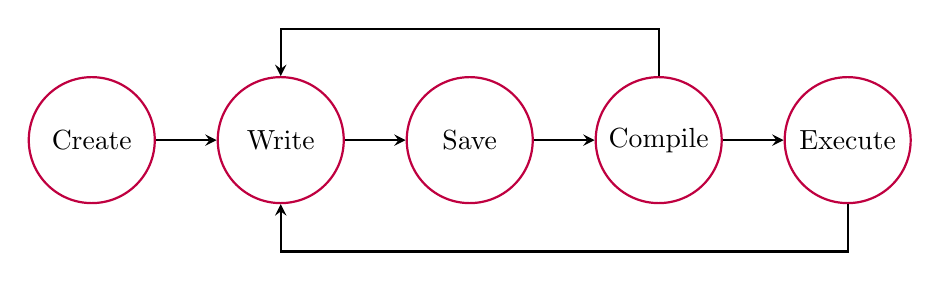
\begin{tikzpicture}[remember picture]
    \newcommand{\stepsize}{24mm}
    \tikzstyle{edge}  = [thick,>=stealth,draw=black]
    \tikzstyle{dedge} = [thick,->,>=stealth,draw=black]
    \tikzstyle{node}=[
      circle,
      draw=purple,
      anchor=center,
      thick,
      minimum size=16mm,
    ]
    
    \node[node] (nCreate) at (0*\stepsize,0) {Create};
    \node[node] (nWrite) at (1*\stepsize,0) {Write};
    \node[node] (nSave) at (2*\stepsize,0) {Save};
    \node[node] (nCompile) at (3*\stepsize,0) {Compile};
    \node[node] (nExecute) at (4*\stepsize,0) {Execute};
    
    \draw[dedge] (nCreate)--(nWrite);
    \draw[dedge] (nWrite)--(nSave);
    \draw[dedge] (nSave)--(nCompile);
    \draw[dedge] (nCompile)--(nExecute);
    \draw[dedge] (nCompile)--([yshift= 6mm]nCompile.north)-|(nWrite);
    \draw[dedge] (nExecute)--([yshift=-6mm]nExecute.south)-|(nWrite);
  \end{tikzpicture}
\end{center}

  \caption{Typical developer cycle.}
  \label{fig:first:phases:cycle}
\end{figure}

\csharpsection{\csharp}

% intro
The program from section \ref{first:writing} looks trivial on the surface, but there happens to be quite a bit more to it that deserves some attention. So, lets give in to it! After all, there are fundamental details at play here that is going to inform our understanding of the \csharp\ programming language.

% compilation
We will start by looking into how \csharp\ code is \idx{compiled}{Compilation} into an \idx{executable}{Executable} binary. This happens in four distinct steps as illustrated in figure \ref{fig:first:csharp:compilation:phases}. The following subsections will cover the role of each of these phases, and give a very short introduction to the mechanisms behind them.

\begin{figure}[tbp]
  \begin{center}
  \scalebox{0.885}{
    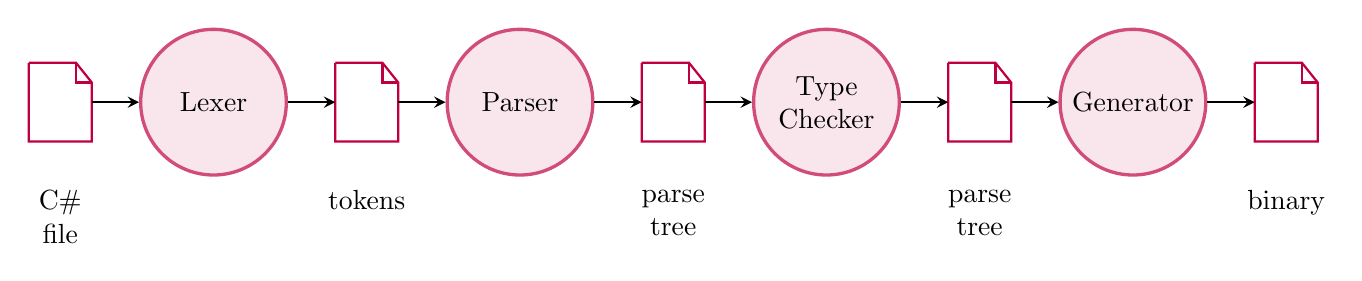
\begin{tikzpicture}[remember picture]
      \newcommand{\spacing}[0]{ 10mm }
      \newcommand{\filesize}[0]{ 0.5 }
      \tikzstyle{edge}  = [thick,>=stealth,draw=black]
      \tikzstyle{dedge} = [thick,->,>=stealth,draw=black]
      \tikzstyle{node}=[
        circle,
        draw=purple!70,
        fill=purple!10,
        anchor=west,
        align=center,
        very thick,
        minimum size=1.85cm
      ]
      \tikzstyle{label}=[
        anchor=north,
        align=center,
      ]
      
      \tikzset{
        pics/file/.style args={#1}{
          code={
            \newcommand{\fileh}[0]{1.0}
            \newcommand{\filew}[0]{0.8}
            \newcommand{\filehc}[0]{\fileh/2}
            \newcommand{\filewc}[0]{\filew/2}
            \draw[-,thick]
              (-\filew *#1, \fileh *#1) to % north west
              ( \filewc*#1, \fileh *#1) to % north east 1
              ( \filew *#1, \filehc*#1) to % north east 2
              ( \filew *#1,-\fileh *#1) to % south east
              (-\filew *#1,-\fileh *#1) to % south west
              (-\filew *#1, \fileh *#1)    % north west
              ;
            \draw[-,thick]
              ( \filewc*#1, \fileh *#1) to
              ( \filewc*#1, \filehc*#1) to
              ( \filew *#1, \filehc*#1)
              ;
          }
        },
      }
      
      % ordinary nodes
      
      \node[node] (lexer)     at (0,0) {Lexer};
      \node[node] (parser)    at ([xshift=2*\spacing]lexer.east) {Parser};
      \node[node] (checker)   at ([xshift=2*\spacing]parser.east) {Type\\Checker};
      \node[node] (generator) at ([xshift=2*\spacing]checker.east) {Generator};
      
      % file nodes
      
      \draw[draw=purple] ([xshift=-\spacing]lexer.west) pic{file={\filesize}};
      \node[label] () at ([xshift=-\spacing,yshift=-2*\filesize*1cm]lexer.west) {\csharp\\file};
      
      \draw[draw=purple] ([xshift=\spacing]lexer.east) pic{file={\filesize}};
      \node[label] () at ([xshift=\spacing,yshift=-2*\filesize*1cm]lexer.east) {tokens};
      
      \draw[draw=purple] ([xshift=\spacing]parser.east) pic{file={\filesize}};
      \node[label] () at ([xshift=\spacing,yshift=-2*\filesize*1cm]parser.east) {parse\\tree};
      
      \draw[draw=purple] ([xshift=\spacing]checker.east) pic{file={\filesize}};
      \node[label] () at ([xshift=\spacing,yshift=-2*\filesize*1cm]checker.east) {parse\\tree};
      
      \draw[draw=purple] ([xshift=\spacing]generator.east) pic{file={\filesize}};
      \node[label] () at ([xshift=\spacing,yshift=-2*\filesize*1cm]generator.east) {binary};
      
      % edges
      
      \draw[dedge] ([xshift=-6mm]lexer.west)--(lexer);
      \draw[dedge] (lexer)--([xshift=6mm]lexer.east);
      
      \draw[dedge] ([xshift=-6mm]parser.west)--(parser);
      \draw[dedge] (parser)--([xshift=6mm]parser.east);
      
      \draw[dedge] ([xshift=-6mm]checker.west)--(checker);
      \draw[dedge] (checker)--([xshift=6mm]checker.east);
      
      \draw[dedge] ([xshift=-6mm]generator.west)--(generator);
      \draw[dedge] (generator)--([xshift=6mm]generator.east);
    \end{tikzpicture}
  }
\end{center}

  \caption{Compilation phases of a \csharp\ program.}
  \label{fig:first:csharp:compilation:phases}
\end{figure}

\subsection{Lexing}

% tokens, token type annotation
The first thing a compiler will do when it sees some code, is to hand it to its \idx{lexer}{Lexer} that then chop it up into a sequence of \idx{tokens}{Token}. This is the only job of the lexer. Each token represents a small part of the code. These parts are atomic units with respect to the following phases of the compilation. By this, we mean that there is no reason for any of the following phases to deal with the code at a higher granularity than this. This may seem very abstract at this point, and that's okay. Lets just say that the output of the lexer is as illustrated in figure \ref{fig:first:hello:tokens}. In this figure, each token is annotated by \idx{type}{Type}. Some are simply named after the character they represent. These include \texttt{RPAR} for right parenthesis and \texttt{SCOLON} for semicolon. Others represent a sequence of characters.

\begin{figure}[tbp]
  \begin{center}
  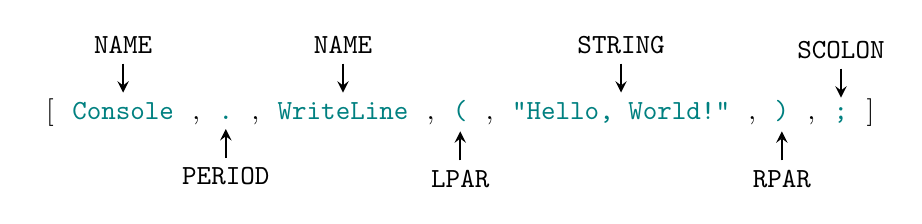
\begin{tikzpicture}[]
    \newcommand{\spacing}[0]{ 6mm }
    \tikzstyle{dedge} = [thick,->,>=stealth,draw=black]
    \tikzstyle{shared}=[
      anchor=base east,
    ]
    \tikzstyle{structure}=[
      shared,
    ]
    \tikzstyle{token}=[
      shared,
      text=teal,
      font=\ttfamily,
    ]
    \tikzstyle{label}=[
      font=\ttfamily,
    ]
    
    \node[matrix,column sep=0mm,anchor=north,] () at (0,0) {
      \node[structure] () {[};
      &
      \node[token] (console) {Console};
      &
      \node[structure] () {,};
      &
      \node[token] (period) {.};
      &
      \node[structure] () {,};
      &
      \node[token] (writeline) {WriteLine};
      &
      \node[structure] () {,};
      &
      \node[token] (lpar) {(};
      &
      \node[structure] () {,};
      &
      \node[token] (string) {"Hello, World!"};
      &
      \node[structure] () {,};
      &
      \node[token] (rpar) {)};
      &
      \node[structure] () {,};
      &
      \node[token] (scolon) {;};
      &
      \node[structure] () {]};
      \\
    };
    
    \node[label] (console label) at ([yshift=\spacing]console.north) {NAME};
    \node[label] (period label) at ([yshift=-\spacing]period.south) {PERIOD};
    \node[label] (writeline label) at ([yshift=\spacing]writeline.north) {NAME};
    \node[label] (lpar label) at ([yshift=-\spacing]lpar.south) {LPAR};
    \node[label] (string label) at ([yshift=\spacing]string.north) {STRING};
    \node[label] (rpar label) at ([yshift=-\spacing]rpar.south) {RPAR};
    \node[label] (scolon label) at ([yshift=\spacing]scolon.north) {SCOLON};
    
    \draw[dedge] (console label)--(console);
    \draw[dedge] (period label)--(period);
    \draw[dedge] (writeline label)--(writeline);
    \draw[dedge] (lpar label)--(lpar);
    \draw[dedge] (string label)--(string);
    \draw[dedge] (rpar label)--(rpar);
    \draw[dedge] (scolon label)--(scolon);
  \end{tikzpicture}
\end{center}

  \caption{Token sequence of the hello-world program produced by the lexer.}
  \label{fig:first:hello:tokens}
\end{figure}

% the name token
\texttt{NAME}, for instance, is our first encounter with the concept of \idx{naming}{Naming}. We will dig more into this as we progress through this book. But for now, lets just say that it is a name which can be used to reference \textsl{something}. Such names are defined by programmers and referenced by programmers having a shared \idx{context}{Context}. In \csharp\ a \texttt{NAME} has to start with either an underscore character or any alphabetic character, and the remaining characters have to be underscores, alphabetic characters or decimal digits.

% the literal token
Another example is \texttt{STRING} (also called a \idx{string literal}{Literal!String}). This is a sequence of arbitrary characters surrounded by quotes. This is a gross simplification. But for now, we don't have to worry about a single detail. Those remaining worries can wait until section \ref{sec:io:strings}.

% escape characters
Naturally, we would like to be able to write whatever text we like in such a string, and that include quotation marks. But if we simply place a quotation mark in there, instead of the comma between \say{\texttt{hello}} and \say{\texttt{world}}, then the lexer would see this quotation mark as the one \idx{terminating}{Termination} the string. And so, a convention has been introduced to solve this problem whereby the \idx{backslash}{Backslash character} character will \textsl{escape} the normal meaning of the following character. We say that the backslash character is an \idx{escape character}{Escape character}. And thus, \say{\texttt{"The \textbackslash " character is used to wrap strings"}} is a valid string. This, of course, puts us in a similarly awkward position when we want to have a backslash character in our string. But here the same solution applies: We simply escape the normal meaning of the backslash character by writing two backslash characters in a row.

\subsection{Grammars}

% introduction
When you read this book, we rely on a shared understanding of the syntax and semantics of the English language. Throughout the book we extend our shared vocabulary with terminology relevant for this particular domain, just like any other textbook. Every language intended for communication between humans has such syntactic rules and a vocabulary. Likewise, every programming language has a \idx{grammar}{Grammar}. It defines what is syntactically valid code.

% dealing with incorrectness
When a written \idx{English}{English} message is used to carry information between humans, the receiving party has the ability to reason about flaws in the \textsl{coding} to that message. When I miss a comma, you will still get the message. A typo is not the end of the world. If I use a word you don't know, then you will look it up, or walk away with perhaps 90\% of the meaning of the offending paragraph. As humans, we are quite robust in terms interpreting text which deviates from the expected format. This is not the case for compilers. When a compiler receives code that does not fit the grammar of the programming language it expects it will outright reject it, and by doing so force you to correct it.

% dumb as a feature
The reason for this is quite simple: While one could make the compiler attempt to guess your intention, this would represent an ambiguity that can have unforeseen consequences. For instance, it could easily change the result of a computation. In section \ref{sec:flow:branch:danglingelse}, we will cover a good example of this. The kind of mess-ups that we see from \idx{generative AI}{AI!Generative} today are simply not acceptable in most production systems. As generative AI dumps the price of low-quality code (e.g., through \idx{vibe coding}{Vibe coding}), we may start to see a shift in peoples mindset and a lowering of expectations. But for now and the foreseeable future, the compiler being dumb should very much be considered a feature.

% specific grammar of hello world example: intro
But lets get back to the hello world example. The specific grammatical rules relevant for understanding how a compiler sees the code are illustrated in syntax \ref{syntax:first:hello} as a railroad diagram. Later on, you might encounter the same information in a textual form called \idx{Backus-Naur Form}{Backus-Naur Form} (or simply BNF). While that format is more relevant for programmatic use, in this book we stick to the visually more appealing \defi{railroad diagram}{Diagram!Railroad}.

\begin{syntaxfloat}
  \begin{syntax}[[xshift=24mm]concept.west]{pgm}
  \SyntaxWestSplit{MainWest}
  \SyntaxEastSplit{MainEast}
  
  \node[nonterminal] (ruleIa) at ($(begin)!0.5!(end)$) {stmts};
  
  \draw[path] (begin)--(ruleIa)--(end);
\end{syntax}
\vspace{-2mm}

\begin{syntax}[[xshift=24mm]concept.west]{stmts}
  \SyntaxWestSplit{MainWest}
  \SyntaxEastSplit{MainEast}
  
  \node[sequence] () at ([yshift=-0*\syntaxruledist]$(begin)!0.5!(end)$) {
    \node[nonterminal]    (ruleIa) {stmt};
    \\
  };
  
  \draw[path] (begin)--(ruleIa)--(end);
  \draw[path] (ruleIa)
            -|([xshift= 0.5*\syntaxruledist,yshift=0.4*\syntaxruledist]ruleIa.east)
            |-(                            [yshift=0.8*\syntaxruledist]ruleIa.center)
            -|([xshift=-0.5*\syntaxruledist,yshift=0.4*\syntaxruledist]ruleIa.west)
            |-(ruleIa);
\end{syntax}
\begin{syntax}[[xshift=24mm]concept.west]{stmt}
  \SyntaxWestSplit{MainWest}
  \SyntaxEastSplit{MainEast}
  
  \node[sequence] () at ([yshift=-0*\syntaxruledist]$(begin)!0.5!(end)$) {
    \node[nonterminal] (ruleIa) {name};
    &
    \node[terminal]    (ruleIb) {.};
    &
    \node[nonterminal] (ruleIc) {name};
    &
    \node[terminal]    (ruleId) {(};
    &
    \node[nonterminal] (ruleIe) {param-list};
    &
    \node[terminal]    (ruleIf) {)};
    &
    \node[terminal]    (ruleIg) {;};
    \\
  };
  
  \draw[path] (begin)--(ruleIa)--(ruleIb)--(ruleIc)--(ruleId)--(ruleIe)--(ruleIf)--(ruleIg)--(end);
\end{syntax}
\begin{syntax}[[xshift=24mm]concept.west]{param-list}
  \SyntaxWestSplit{MainWest}
  \SyntaxEastSplit{MainEast}
  
  \node[sequence] () at ([yshift=-1*\syntaxruledist]$(begin)!0.5!(end)$) {
    \node[nonterminal] (ruleIa) {expr};
    \\
  };
  \node[sequence] () at ([yshift=-2*\syntaxruledist]$(begin)!0.5!(end)$) {
    \node[terminal] (ruleIIa) {,};
    \\
  };
  
  \draw[path] (begin)--(end);
  \draw[path] (begin) to[-|-] (ruleIa) to[-|-] (end);
  \draw[path] (ruleIa)
            -|([xshift= 0.5*\syntaxruledist,yshift=-0.5*\syntaxruledist]ruleIa.east)
            |-(                            [yshift=0.0*\syntaxruledist]ruleIIa.east);
  \draw[path] (ruleIIa)
            -|([xshift=-0.5*\syntaxruledist,yshift=-0.5*\syntaxruledist]ruleIa.west)
            |-(                            [yshift=0.0*\syntaxruledist]ruleIa.west);
\end{syntax}
\begin{syntax}[[xshift=24mm]concept.west]{expr}
  \SyntaxWestSplit{MainWest}
  \SyntaxEastSplit{MainEast}
  
  \node[sequence] () at ([yshift=-0*\syntaxruledist]$(begin)!0.5!(end)$) {
    \node[nonterminal]    (ruleIa) {string-lit};
    \\
  };
  
  \draw[path] (begin)--(ruleIa)--(end);
\end{syntax}
%\begin{syntax}[[xshift=24mm]concept.west]{name}
%  \SyntaxWestSplit{MainWest}
%  \SyntaxEastSplit{MainEast}
%  
%  \coordinate (head) at ($(begin)!1/3!(end)$);
%  \coordinate (tail) at ($(begin)!2/3!(end)$);
%  \coordinate (center) at ($(begin)!0.5!(end)$);
%  \coordinate (tailcenter) at ($(begin)!2.5/3!(end)$);
%  
%  \node[terminal]    (ruleIa) at ([yshift= 0.5*\syntaxruledist]head) {\_};
%  \node[nonterminal] (ruleIb) at ([yshift=-0.5*\syntaxruledist]head) {azAZ};
%  \node[terminal]    (ruleIIa) at ([yshift= 1.0*\syntaxruledist]tail) {\_};
%  \node[nonterminal] (ruleIIb) at ([yshift= 0.0*\syntaxruledist]tail) {azAZ};
%  \node[nonterminal] (ruleIIc) at ([yshift=-1.0*\syntaxruledist]tail) {09};
%  
%  % head west
%  \draw[path] (begin)
%            --($([xshift=-0.5*\syntaxruledist]ruleIb.west |- begin)$)
%            |-(ruleIa.west);
%  \draw[path] (begin)
%            --($([xshift=-0.5*\syntaxruledist]ruleIb.west |- begin)$)
%            |-(ruleIb.west);
%  
%  % head east
%  \draw[path] (ruleIa.east)
%            --($([xshift=0.5*\syntaxruledist]ruleIb.east |- ruleIa)$)
%            |-(ruleIIb.west);
%  \draw[path] (ruleIb.east)
%            --([xshift=0.5*\syntaxruledist]ruleIb.east)
%            |-(ruleIIb.west);
%  
%  % tail west
%  \draw[path] (center)
%            --([xshift=-0.5*\syntaxruledist]ruleIIb.west)
%            |-(ruleIIa);
%  \draw[path] (center)
%            --([xshift=-0.5*\syntaxruledist]ruleIIb.west)
%            |-(ruleIIc);
%  
%  % tail east
%  \draw[path] (ruleIIb.east)--(end);
%  \draw[path] (ruleIIa.east)
%            --($([xshift=0.5*\syntaxruledist]ruleIIb.east |- ruleIIa)$)
%            |-(end);
%  \draw[path] (ruleIIc.east)
%            --($([xshift=0.5*\syntaxruledist]ruleIIb.east |- ruleIIc)$)
%            |-(end);
%  
%  % tail bypass
%  \draw[path] (center)
%            --([xshift=-0.5*\syntaxruledist]ruleIIb.west)
%            |-([yshift=-1.8*\syntaxruledist]ruleIIb.center)
%            -|([xshift= 0.5*\syntaxruledist]ruleIIb.east)
%            --(end);
%  
%  % tail loop
%  \draw[path] (ruleIIb.east)
%            --(tailcenter)
%            |-([yshift= 1.8*\syntaxruledist]ruleIIb.center)
%            -|(center)
%            --(ruleIIb.west);
%  
%\end{syntax}

  \caption{Concepts involved in the basic hello-world program}
  \label{syntax:first:hello}
\end{syntaxfloat}

% concepts, tracks, pgm example
This grammar defines five grammatical concepts, namely \conceptname{pgm}, \conceptname{stmt}, \conceptname{param-list}, \conceptname{expr} and \conceptname{name}. Each of these definitions define the valid sequences of tokens from an empty circle on the left to a filled circle on the right. We read these by following the tracks. The program itself (or \conceptname{pgm}) thus has to contain a sequence of at least one statement (or \conceptname{stmt}). This, due to the loop around \conceptname{stmt}, as defined in the intermediary \conceptname{stmts}.

% stmt concept, param-list concept
The next rule unfolds what a statement is. A statement must consist of a name followed by a period followed by another name followed by a left parenthesis followed by a parameter list (or \conceptname{param-list}) followed by a right parenthesis followed by a semicolon. The next rule states that this \conceptname{param-list} is either empty, or a sequence of expressions (\conceptname{expr}) with commas in between. The \conceptname{expr} has to be a string literal (\conceptname{string-lit}).

% terminals and nonterminals
By now, you should have noticed the two different types of nodes in the diagram. One type, the \idx{terminals}{Terminal!Grammar context}, represents a single token like a comma or a left parenthesis. The other type, the \idx{nonterminals}{Nonterminal}, represents another concept that can be unfolded or expanded. So, why those names in particular? This has to do with wether the node in question \textsl{terminates} the unfolding of concept nodes: While a program is a complex thing that can take many forms and needs further detailing to be fully described, a comma is simply a comma.

\subsection{Parsing}

% parse tree
That sequence of tokens is fed into the \idx{parser}{Parser}. Informed by the grammar of the language, the parser finds a unique application of the rules that match the sequence of tokens. The result is a tree structure called a \idx{parse tree}{Parse tree}. Each unfolding of a rule results in child nodes being added to the tree. The hello world program results in the parse tree of figure \ref{fig:first:hello:parsetree}. The parse tree contains only those elements whose values could vary from rule application to rule application. So, each comma or parenthesis is left out. Should the parser fail to produce a parse tree from its input tokens, then it will \idx{exit}{Exit} with a \idx{parse error}{Error!Parse}.

\begin{figure}[tbp]
  \begin{center}
  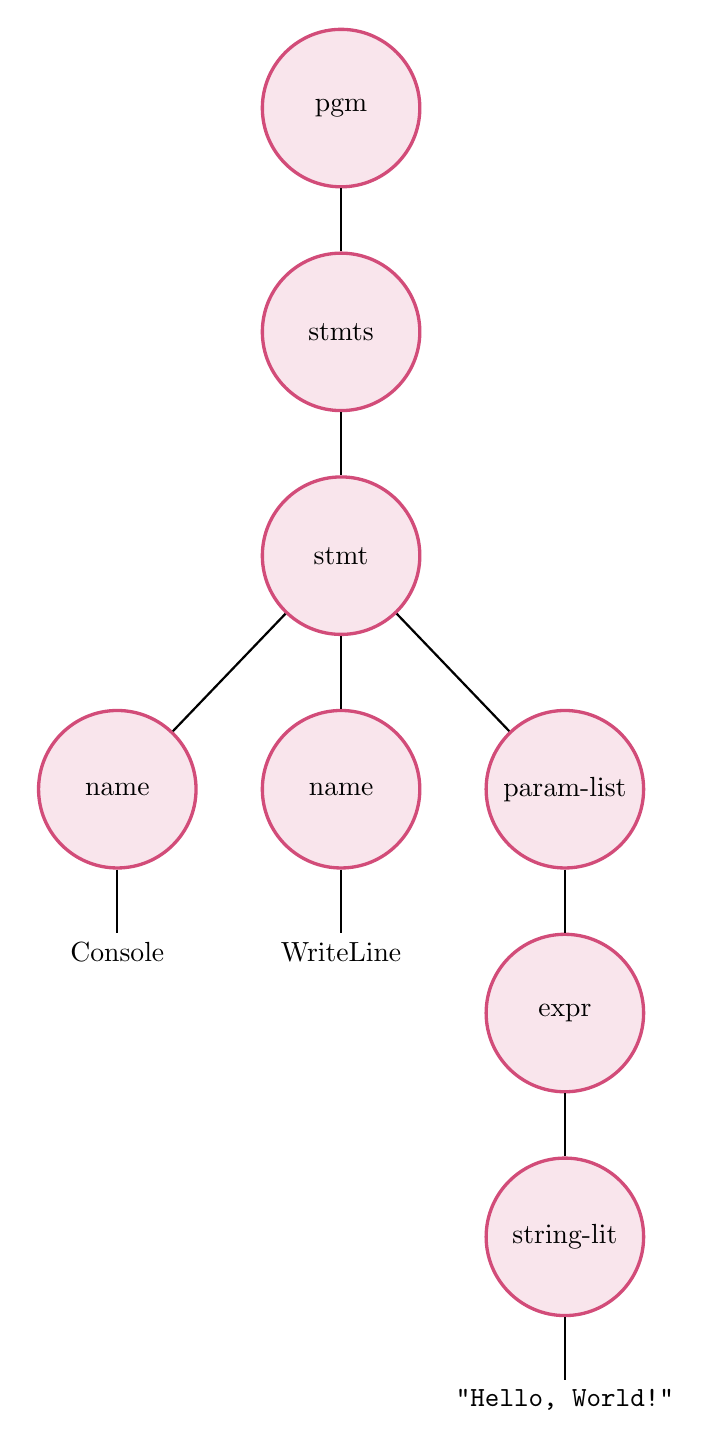
\begin{tikzpicture}[]
    \newcommand{\spacing}[0]{ 8mm }
    \tikzstyle{edge}  = [thick,>=stealth,draw=black]
    \tikzstyle{dedge} = [thick,->,>=stealth,draw=black]
    \tikzstyle{terminal}=[
      anchor=north,
    ]
    \tikzstyle{nonterminal}=[
      circle,
      draw=purple!70,
      fill=purple!10,
      anchor=north,
      very thick,
      minimum size=2.0cm
    ]
    
    \node[nonterminal] (pgm) at (0,0) {pgm};
    \node[nonterminal] (stmts) at ([yshift=-\spacing]pgm.south) {stmts};
    \node[nonterminal] (stmt) at ([yshift=-\spacing]stmts.south) {stmt};
    \node[matrix,column sep=\spacing,anchor=north,] () at ([yshift=-\spacing]stmt.south) {
      \node[nonterminal] (context) {name};
      &
      \node[nonterminal] (function) {name};
      &
      \node[nonterminal] (params) {param-list};
      \\
    };
    \node[terminal] (context value)  at ([yshift=-\spacing]context.south) {Console};
    \node[terminal] (function value) at ([yshift=-\spacing]function.south) {WriteLine};
    \node[nonterminal] (params expr)   at ([yshift=-\spacing]params.south) {expr};
    \node[nonterminal] (string)   at ([yshift=-\spacing]params expr.south) {string-lit};
    \node[terminal] (string value)   at ([yshift=-\spacing]string.south) {\texttt{"Hello, World!"}};
    
    \draw[edge] (pgm)--(stmts);
    \draw[edge] (stmts)--(stmt);
    \draw[edge] (stmt)--(context);
    \draw[edge] (stmt)--(function);
    \draw[edge] (stmt)--(params);
    \draw[edge] (context)--(context value);
    \draw[edge] (function)--(function value);
    \draw[edge] (params)--(params expr);
    \draw[edge] (params expr)--(string);
    \draw[edge] (string)--(string value);
  \end{tikzpicture}
\end{center}

  \caption{Parse tree of hello-world program.}
  \label{fig:first:hello:parsetree}
\end{figure}

\subsection{Type Checker}

% statements, expressions, types
When the final program is executing, the parts of that program that comes from an expression will \idx{evaluate}{Evaluation} to some value. The parts that comes from a statement does not. As we will see in the next chapter, any value has a type. Many of the grammatical rules that deal with expression have restrictions on the types of those expressions. For instance, you can divide a number by another number, but not by a string (such as \texttt{"Hello, World!"}).

% type checker
The parse tree is fed into yet another component of the compiler called a \idx{type checker}{Type checker}. The type checker has access to a suite of type rules. It's job is to verify that none of them are violated. Any violation is a \idx{type error}{Error!Type}.

\subsection{Compilation}

% downplay importance, production of binary code that can be executed on a processor, that processor is virtual but still a processor, the virtual machine has a lot of intricacies
The binary output of the compilation maintains much of the structure of the parse tree. In fact, the structure of the parse tree defines \textsl{how} the binary will be evaluated, when \idx{executed}{Execution} by the \idx{processor}{Processor}. This processor is, in the case of \csharp a logical one rather than a physical one; it is implemented in code as a \idx{virtual machine}{Virtual machine} and essentially runs as a program on top of your operating system. That means that the binary can be executed on any architecture as long as a matching virtual machine is available for it. Such virtual machines have lots of intricacies, but we will leave them out of this book.

\subsection{Importance}

% point
While it is not critical to understand these intricacies in your day-to-day practice as a programmer, they do a great job at helping you \idx{reason}{Reason} about what you experience, and that saves you a lot of both effort and frustration. The takeaway should be that the compiler goes through a number of phases. Each of these have a distinct function and if you provide the compiler with invalid input (i.e., your source code), one of them will fail.

% final words on the grammar so far
As we move through this book, and broaden our understanding of the \csharp\ language, we will extend on this grammar. The pgm definition will receive one extension and both stmt and expr will receive many. We settle for these definitions being \textsl{mostly} correct as the correct rules are at least an order of magnitude more complicated, and this complexity is disruptive for understanding of the language at this level.

\pythonsection{Python}
\label{sec:first:python}

In Python, the equivalent program looks like this:

\includePythonFile{first/hello/hello.py}

In order to execute this script, we first need to make the file \idx{executable}{File!Executable}:
\begin{minted}[]{shell-session}
aslak@gaia:/tmp/python_hello$ chmod u+x hello.py
\end{minted}

That first line of the Python source code is called a \idx{shebang}{Shebang} after the first two characters. When executing, this line uses the \filename{/bin/env} program to look up an appropriate interpreter for \filename{python3} and then feed the remaining lines to it. This is known as a \idx{dispatch mechanism}{Dispatch mechanism}. The development cycle is very similar to \csharp\ except that there is neither an initial project creation step or a separate compilation step. Running the program is done like so:

\begin{minted}[]{shell-session}
aslak@gaia:/tmp/python_hello$ ./hello.py
Hello, World!
\end{minted}

The Python interpreter has an \idx{interactive mode}{Mode!Interactive} that we can \idx{invoke}{Invoke} directly:

\begin{minted}[]{shell-session}
aslak@gaia:/tmp/python_hello$ /bin/env python3
Python 3.13.3 (main, Apr 10 2025, 21:38:51) [GCC 14.2.0] on linux
Type "help", "copyright", "credits" or "license" for more information.
>>> print("Hello, World!")
Hello, World!
>>> 
\end{minted}

On the first line we invoke the interpreter. Then, it -- exactly as our shell -- presents us with a prompt. This prompt allows us to \idx{issue}{Issue} python commands. The interactive mode is typically used for rapid experimentation. Such an interactive mode is commonly known as a \defi{REPL}{REPL} (\underline{r}equest-\underline{e}val-\underline{p}rint-\underline{l}oop). That is, a program that requests a line of input from the user, evaluates that line, prints out the result and loops back to requesting a new line.

Another way to write python code is though a \idx{notebook}{Notebook} environment. Such an environment is usually provided through a browser by a system such as \idx{Jupyter}{Jypyter}. In such an environment, code is split up into cells and these cells are laid out in a sequence. Any cell can build on the code that is introduced in previous cells and the code in these cells have easily accessible means for producing visual outputs. The workflow is essentially the same as for \csharp\ except that notebooks are usually saved automatically.

\csection{C}

The minimal hello world program in C looks (more or less) like this:

\includeCFile{first/hello/hello.c}

This version immediately looks a lot more complicated! So, why is that? Well, lets try to disect it \ldots

\subsection{Explanation}

% first line
Most \idx{general-purpose languages}{Language!General-purpose} (like \csharp, C, Python and Elixir) come with a sizeable \idx{library}{Library} of functionality. While all of this is available to you as a programmer there are downsides to having it all adirectly available all the time. To simplify grossly, it is a situation similar to finding a specific needle in a stack of slighty different needles. The first line tells C -- or rather the C preprocessor -- to include the definitions present in the \filename{stdio.h} file. This pulls in, amongst others, the \funcname{printf} function, that can print stuff to the screen for us.

% main function
Wrapping use of that \funcname{printf} function is the declaration of \funcname{main}. This is the main entry point of the program. That means that this is where the execution of the program starts. It informs the program of how many options have been passed to it (through \varname{argc}) and what those options are (through \varname{argv}). This is \idx{kernels}{Kernel} primary means of informing a program of what inputs it should operate on. The \typename{int} before \funcname{main} indicates that the program evaluates to an integer value. It is convention that a zero indicates success and a non-zero value functions an an \idx{error code}{Error code}. As this program doesn't explicitly return such a number, it will default to zero.

It is important to point out that \csharp\ supports a very similar program structure. After all, this is how the kernel passes options to a program. Any language that supports such options will have something similar. It is typically in a \idx{\funcname{main} function}{Function!Main}. But sometimes it is implicit or has to be actively \idx{imported}{Importing}. That is not likely to mean much to you at this point, and that is okay.

\subsection{Workflow}

In order to compile the code to an executable binary we need to invoke a compiler. Lets use the \commandname{clang} compiler and explicitly name the file that should hold the resulting binary:

\begin{minted}[]{shell-session}
aslak@gaia:/tmp/c_hello$ clang hello.c -o hello
\end{minted}

One key difference, compared to \csharp, is that C compiles to a \defi{native binary}{Binary!Native}. That is a binary that follows a format that is directly compatible with the processor architecture of your computer. We notice this when executing the code. With \csharp we used \commandname{dotnet} to essentially simulate a virtual machine that was capable of interpreting the intermediate language binary. This manifested as a command that began with \commandname{dotnet}.

The \commandname{dotnet} program that is then invoked is another example of a native binary. So, we can invoke the binary that we have built from our C code in exactly the same way. However, unlike \commandname{dotnet}, our binary is not in the \idx{path}{Path}. That means that we need an \idx{explicit path}{Path!Explicit} to it. That is accomplished by prefacing it with \filename{./}, like so:

\begin{minted}[]{shell-session}
aslak@gaia:/tmp/c_hello$ ./hello
Hello, World!
\end{minted}

\elixirsection{Elixir}

\subsection{Interpretation}

Elixir code can be executed through an interpreter (like Python), it can be worked on through a notebook system (like Python) and it can be executed on a virtual machine (like \csharp). This virtual machine is called \idx{BEAM}{BEAM}. Unlike that for \csharp, it is a \idx{distributed}{Virtual machine!Distributed} virtual machine. The hello world program looks slightly different depending on whether a separate compilation phase is used or the code is interpreted. For the script version, the it looks like this:

\includeElixirFile{first/hello/hello.exs}

% transition to REPL
As with the Python script (in section \ref{sec:first:python}) it uses a \idx{shebang}{Shebang} mechanism. For that mechanism to work it needs to be \idx{executable}{Executable}. However, while the interpreter for the script is called \commandname{elixir} this is not the case for the REPL. The interpreter for the REPL is called \commandname{iex}:

\begin{minted}[breaklines]{shell-session}
aslak@gaia:/tmp/elixir_hello$ iex
Erlang/OTP 27 [erts-15.2.1] [source] [64-bit] [smp:16:16] [ds:16:16:10] [async-threads:1] [jit:ns]

Interactive Elixir (1.18.2) - press Ctrl+C to exit (type h() ENTER for help)
iex(1)> IO.puts("Hello, World!")
Hello, World!
:ok
iex(2)> 
\end{minted}
The line that makes the printout appear is still the same. Here, you see it appear after a \idx{prompt}{Prompt}. The \commandname{iex} prompt is, unlike the Python one numbered. Also, everything in Elixir evaluated to a value, and the \idx{REPL}{REPL} prints out this value after having evaluated a line. In this case \texttt{IO.puts("Hello, World!")}, after having performed its function of printing \quoted{Hello, World!} to the screen, evaluates to \texttt{:ok}.

\subsection{Compilation}

% mix creating new project
Like \csharp, Elixir has a notion of a project. A new project can be started using the \commandname{mix} command like so:

\begin{minted}[breaklines]{shell-session}
aslak@gaia:/tmp/elixir$ mix new hello
* creating README.md
* creating .formatter.exs
* creating .gitignore
* creating mix.exs
* creating lib
* creating lib/hello.ex
* creating test
* creating test/test_helper.exs
* creating test/hello_test.exs

Your Mix project was created successfully.
You can use "mix" to compile it, test it, and more:

    cd hello
    mix test

Run "mix help" for more commands
\end{minted}

Lets \commandname{cd} to the newly created directory and make sure that \filename{lib/hello.ex} contains the following code:

\includeElixirFile{first/hello_compiled/lib/hello.ex}

We can compile the project using the following \commandname{mix} command:

\begin{minted}[breaklines]{shell-session}
aslak@gaia:/tmp/elixir/hello$ mix compile
Compiling 1 file (.ex)
Generated hello app
\end{minted}

The BEAM virtual machine is in some ways more complex than the \idx{CLR}{CLR}. One such way is that it can run multiple applications at the same time. In order to do so, we need to define an \idx{application}{Application} in our \idx{project}{Project} and tell it to invoke our \funcname{Hello.hello} function. This, however, is not an Elixir book, and that is a detail that does not help us progress.

% interpreter with access to new project
You should note that the project does compile. One reason for that is that we can use the compiled code through our REPL. We do this by passing the \commandname{-S mix} paramter along to our \commandname{iex} command:

\begin{minted}[breaklines]{shell-session}
aslak@gaia:/tmp/elixir/hello$ iex -S mix
Erlang/OTP 27 [erts-15.2.1] [source] [64-bit] [smp:16:16] [ds:16:16:10] [async-threads:1] [jit:ns]

Interactive Elixir (1.18.2) - press Ctrl+C to exit (type h() ENTER for help)
iex(1)> Hello.hello()
Hello, World
:ok
\end{minted}

\subsection{Notebook}

% livebook
Like Python, Elixir code can run in notebook form. Unlike Python, we will actually be using this later on. So, lets see what it looks like in \idx{Livebook}{Livebook}, the Elixir application for editing and executing notebooks.

% interface walkthrough: main page, new workbook
Once started, the Livebook program exposes a webserver that hosts a webapp. Point a browser at the URL of this webserver and you will be greated by the webapp. Depending on the specific version you should see something like the screenshot of figure \ref{fig:first:elixir:livebook:main}. At the top righthand corner there is a blue button labeled \say{+ New notebook}. Next to it you will find a button labeled \say{Open} that you can upse to open a previously saved notebook. Click the first button to create a new notebook.

\begin{figure}[tbp]
  
  \caption{Screenshot of the main page of Livebook.}
  \label{fig:first:elixir:livebook:main}
\end{figure}

% configuring livebook: ligatures, automatic close brackets
Livebook has a few settings that we would like to change in order to improve our experience. To do so, open up Livebook, go to Settings and scroll down to the \say{Code Editer} segment. Make sure that:
\begin{itemize}
  \item \textbf{\textsl{Automatically close brackets}} is disabled.
  \item \textbf{\textsl{Render ligatures}} is enabled.
\end{itemize}

\begin{figure}[tbp]
  
  \caption{Screenshot of the configuration page of Livebook.}
  \label{fig:first:elixir:livebook:config}
\end{figure}

% interface walkthrough: code cells, evaluation, automatic evaluation, status indicators, saving

\begin{figure}[tbp]
  
  \caption{Screenshot of a notebook in Livebook.}
  \label{fig:first:elixir:livebook:notebook}
\end{figure}

\subsection{Clustering}

% interpreter/livebook hooking into other virtual machine

First, we need to start a named node and provide it with a cookie (read: secret). There are a number of ways to accomplish this, but the easiest one is to start a new REPL session using the \commandname{iex} command with a few parameters:

\begin{minted}[breaklines]{shell-session}
aslak@gaia:/tmp/elixir/hello$ iex --name test@127.0.0.1 --cookie mycookie 
Erlang/OTP 27 [erts-15.2.5] [source] [64-bit] [smp:16:16] [ds:16:16:10] [async-threads:1] [jit:ns]

Interactive Elixir (1.18.3) - press Ctrl+C to exit (type h() ENTER for help)
iex(test@127.0.0.1)1>
\end{minted}

Then, create a new notebook in Livebook and add four Elixir code cells to it. In the first cell we make the node hosting the livebook connect to the node of the REPL (this only has to be accomplished once):

\begin{minted}[breaklines]{elixir}
node = :"test@127.0.0.1"
cookie = :mycookie

Node.set_cookie(node, cookie)
Node.connect(node)
Node.alive?()
\end{minted}

This should evaluate to \valuename{true}. Next, we can run some code on the node we just connected to. In this case, we wait for a message of a particular format to be received and send back an appropriate response:

\begin{minted}[breaklines]{elixir}
pid = Node.spawn_link node, fn ->
  receive do
    {:ping, org_pid} -> send org_pid, {:pong, "Hello, World"}
  end
end
\end{minted}

The third cell contains code for sending a message containing the process ID of the current process to the process that we just started on the other node. The code for this is:

\begin{minted}[breaklines]{elixir}
send pid, {:ping, self()}
\end{minted}

At this point we can use the fourth cell to wait for a message to arrive:

\begin{minted}[breaklines]{elixir}
receive do
  message -> message
end
\end{minted}

\textbf{Note:} This is a very simple example of how code can communicate across a clustered virtual machine. While this may seem overwhelming to you now, it can both get much more complicated and much more beneficial.

\section{Summary}

% ref to fig, what does that mean? Is it better to have more boxes checked? Why and why not?
The covered languages support for \idx{execution models}{Execution model} is summarized in figure \ref{fig:first:phases:summary}. C and \csharp\ only support a single model each, while Elixir supports 5 (or 3 with variations). Does that mean that Elixir is a superior language? No, certainly not. But it does mean that you have more options as to how you execute Elixir code. Sometimes support for specific execution models matter, but often it does not.

\begin{figure}[tbp]
  \begin{center}
  \begin{tabular}{ccccl}
    \rotatebox{90}{\textbf{C}} & \rotatebox{90}{\textbf{\csharp}} & \rotatebox{90}{\textbf{Python}} & \rotatebox{90}{\textbf{Elixir}} & \textbf{Execution model} \\
    $\times$ & & & & Compile and execute directly on hardware \\
    & $\times$ & & $\times$ & Compile and execute in VM \\
    & & $\times$ & $\times$ & Script \\
    & & $\times$ & $\times$ & REPL \\
    & & $\times$ & $\times$ & Notebook \\
    & & & $\times$ & Script attached to running VM \\
    & & & $\times$ & REPL attached to running VM \\
    & & & $\times$ & Notebook attached to running VM \\
  \end{tabular}
\end{center}

  \caption{Summary of execution models of various programming languages.}
  \label{fig:first:phases:summary}
\end{figure}

% tradeoffs
It is also important to point out that the design of a programming language is riddled with \idx{tradeoffs}{Tradeoff}, and these are often resolved in very different ways. That results in some set of qualities, of which the supported set of execution models are found. As a developer, it will be your job to decide which combination of qualities are needed to maximize \idx{value}{Value} for a given project, and based on that choose a language.

\exercises{first}{The First Program}


\chapter{Primitive Types}

\section{Numbers}

% everything is a number, not always obvious, classes of numbers, the simples calls is integers
All values that we may want to work with in a computer are, one way or the other, \idx{numbers}{Number}. This fact may not always be obvious, but it will be quite a while before you encounter such examples. From public school and highschool, we know these classes of numbers:
\begin{itemize}
  \descitem{The \idx{natural numbers}{Numbers!Natural}} ($\mathbb{N}$) These are the non-negative numbers that can be written without a decimal point\footnote{There are two definitions of natural numbers. The other definition is that they are the positive numbers that can be written without a decimal point. That is to say, without zero. As this definition is generally less applicable in computers, we stick to the first definition.}.
  \descitem{The \idx{integers}{Numbers!Integer}} ($\mathbb{Z}$) These are all the natural numbers (according to the first definition) along with the negative versions of the natural numbers (according to the second definition). That definition juggling is to make sure that we don't have a negative zero.
  \descitem{The \idx{real numbers}{Numbers!Real}} ($\mathbb{R}$) These are all the numbers that can be placed on a line between $-\infty$ and $\infty$. We often refer to these as floating point numbers.
  \descitem{The \idx{rational numbers}{Numbers!Rational}} ($\mathbb{Q}$) These are then numbers that can be written as the fraction $m/n$ where $m \in \mathbb{Z}$ and $m \in \mathbb{N}$.
  \descitem{The \idx{irrational numbers}{Numbers!Irrational}} ($\mathbb{P}$) These are numbers that belong to $\mathbb{R}$ but not $\mathbb{Q}$. This is where $\pi$ and $e$ belong.
\end{itemize}
Computers typically works with other classes of numbers. In the following sections, we will explore the most commonly used ones. Common to these is that they are all \idx{represented in binary}{Representation!Binary} numbers. That is, using the \idx{base-2}{Base 2} digits. We are used to working with \idx{base-10}{Base 10} where numbers are digits between zero and nine. In base-2, the numbers are made up of digits between zero and one (i.e., \texttt{0} or \texttt{1}). Such a digit is called a \defi{bit}{Bit}, and a sequence of eight bits is referred to as a \defi{byte}{Byte}. The plural forms of the singular bit and byte is bits and bytes. Bits are, by the way, the \idx{SI unit}{SI unit} of information, in the same way as meter is the SI unit of distance. Accordingly, we measure \idx{information}{Information} in bits.

\section{Integers}

% how we know them (no decimal point), what we use them for (typically counts and variants thereof)
We recognize integers as numbers without a decimal point. We use them for counting, and variants thereof. A human may have two or three siblings. But if I were to tell you that I know someone who has 2.3 siblings then you would begin to question my faculties.

\subsection{Operations}

% basic operations
All general purpose languages support the four basic \idx{arithmetic operators}{Operation!Arithmetic} for addition, subtraction, multiplication and division of integers. The tree first of these will guarantee an integral result. For instance, if you add two integers, you will get an integer. The \textsl{size} of this integer may be affected though. But more on that in section \ref{primitives:int:representation}.

% that division thing
That rule, about the result of an operation resulting in an integral value does not hold for the \idx{division}{Operation!Division} operation though. Mathematically, the result \textsl{may} be integral, but generally speaking there is no guarantee, and more often than not it is simply not the case. Most programming languages supports two types of division; namely \idx{integer division}{Operation!Division!Integer} and \idx{floating-point division}{Operation!Division!Floating-point}. The result of a floating-point division is a floating-point number as introduced in section \ref{primitives:float}. The result of an integer division is an integer.

% remainder vs modulo
This operation is tightly coupled to both the \idx{remainder}{Remainder} and the \idx{modulo}{Modulo} operations. The difference between these is how they handle negative numbers.

% TODO: Figure of remainder vs modulo

\subsection{Representation}
\label{primitives:int:representation}

% intro: decimal (least significant digit to the right, 10 values for each digit, 10x difference between significance of neighboring digits), same for binary
We all know the \idx{decimal numeral system}{Decimal numeral system}. That is, the way we represent numbers using \idx{base-10}{Base-10} positioning of digits. In the west, we write the least significant digit to the right. There are ten potential values for each digit and a 10x order of magnitude between two successive digits. The same goes for \idx{binary}{Binary} (or \idx{base-2}{Base-2}). We write the least significant digit to the right, we have two potential values for each digit (zero and one), and the difference between two neighboring digits is a factor of two. Binary values are often \idx{prefixed}{Prefix!Number} by \say{0b}. Figure \ref{fig:prim:int:repr:base} illustrates how to interpret a binary number.

\begin{figure}[tbp]
  \begin{center}
  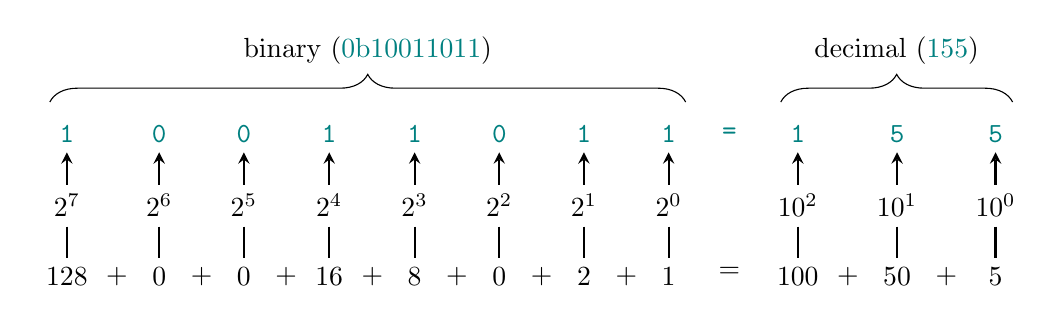
\begin{tikzpicture}[]
    \newcommand{\spacing}[0]{ 4mm }
    \tikzstyle{edge} = [thick ,draw=black]
    \tikzstyle{dedge} = [thick,->,>=stealth,draw=black]
    \tikzstyle{shared}=[
      anchor=center,
    ]
    \tikzstyle{structure}=[
      shared,
    ]
    \tikzstyle{digit}=[
      shared,
      text=teal,
      font=\ttfamily,
    ]
    \tikzstyle{label}=[
      font=\ttfamily,
    ]
    
    \node[matrix,row sep=\spacing,column sep=0mm,anchor=north,] () at (0,0) {
      % representations
      \node[digit] (bseven) {1};
      &
      &
      \node[digit] (bsix)   {0};
      &
      &
      \node[digit] (bfive)  {0};
      &
      &
      \node[digit] (bfour)  {1};
      &
      &
      \node[digit] (bthree) {1};
      &
      &
      \node[digit] (btwo)   {0};
      &
      &
      \node[digit] (bone)   {1};
      &
      &
      \node[digit] (bzero)  {1};
      &
      \node[label] (spacing spacing spacing) {\hspace{4mm}};
      &
      \node[digit] ()       {=};
      &
      \node[label] (spacing spacing spacing) {\hspace{4mm}};
      &
      \node[digit] (dtwo)   {1};
      &
      &
      \node[digit] (done)   {5};
      &
      &
      \node[digit] (dzero)  {5};
      \\
      
      % units
      \node[label] (bseven label) {$2^7$};
      &
      &
      \node[label] (bsix label)   {$2^6$};
      &
      &
      \node[label] (bfive label)  {$2^5$};
      &
      &
      \node[label] (bfour label)  {$2^4$};
      &
      &
      \node[label] (bthree label) {$2^3$};
      &
      &
      \node[label] (btwo label)   {$2^2$};
      &
      &
      \node[label] (bone label)   {$2^1$};
      &
      &
      \node[label] (bzero label)  {$2^0$};
      &
      &
      &
      &
      \node[label] (dtwo label)   {$10^2$};
      &
      &
      \node[label] (done label)   {$10^1$};
      &
      &
      \node[label] (dzero label)  {$10^0$};
      \\
      
      % values
      \node[label] (bseven value) {$128$};
      &
      \node[label] () {$+$};
      &
      \node[label] (bsix value)   {$0$};
      &
      \node[label] () {$+$};
      &
      \node[label] (bfive value)  {$0$};
      &
      \node[label] () {$+$};
      &
      \node[label] (bfour value)  {$16$};
      &
      \node[label] () {$+$};
      &
      \node[label] (bthree value) {$8$};
      &
      \node[label] () {$+$};
      &
      \node[label] (btwo value)   {$0$};
      &
      \node[label] () {$+$};
      &
      \node[label] (bone value)   {$2$};
      &
      \node[label] () {$+$};
      &
      \node[label] (bzero value)  {$1$};
      &
      &
      \node[label] () {$=$};
      &
      &
      \node[label] (dtwo value)   {$100$};
      &
      \node[label] () {$+$};
      &
      \node[label] (done value)   {$50$};
      &
      \node[label] () {$+$};
      &
      \node[label] (dzero value)  {$5$};
      \\
    };
    
    \draw[dedge] (bseven label)--(bseven);
    \draw[dedge] (bsix label)  --(bsix);
    \draw[dedge] (bfive label) --(bfive);
    \draw[dedge] (bfour label) --(bfour);
    \draw[dedge] (bthree label)--(bthree);
    \draw[dedge] (btwo label)  --(btwo);
    \draw[dedge] (bone label)  --(bone);
    \draw[dedge] (bzero label) --(bzero);
    \draw[dedge] (dtwo label)  --(dtwo);
    \draw[dedge] (done label)  --(done);
    \draw[dedge] (dzero label) --(dzero);
    
    \draw[edge] (bseven label)--(bseven value);
    \draw[edge] (bsix label)  --(bsix value);
    \draw[edge] (bfive label) --(bfive value);
    \draw[edge] (bfour label) --(bfour value);
    \draw[edge] (bthree label)--(bthree value);
    \draw[edge] (btwo label)  --(btwo value);
    \draw[edge] (bone label)  --(bone value);
    \draw[edge] (bzero label) --(bzero value);
    \draw[edge] (dtwo label)  --(dtwo value);
    \draw[edge] (done label)  --(done value);
    \draw[edge] (dzero label) --(dzero value);
    
    \draw[decorate,decoration={brace, amplitude=10pt, raise=5pt}] (bseven.north west) to node[black,midway,above=15pt] {binary (\textcolor{teal}{0b10011011})} (bzero.north east);
    \draw[decorate,decoration={brace, amplitude=10pt, raise=5pt}] (dtwo.north west) to node[black,midway,above=15pt] {decimal (\textcolor{teal}{155})} (dzero.north east);
  \end{tikzpicture}
\end{center}

  \caption{Representation of numbers in decimal and binary.}
  \label{fig:prim:int:repr:base}
\end{figure}

% integer size
Normally, when we write out a number, we don't care about how much space it takes up. We have a need to represent the number and it takes up the space it takes up. Space is not an issue. But in a computer, that number need to be worked on by the machine (see section \ref{sec:machine}). The \idx{ALU}{ALU} has to be designed for parameters of a specific number of bits, and the instructions for loading and storing register values have to be designed for a specific number of bits. While the hardware support doesn't necessarily put hard restrictions on what we can do, it does dictate which sizes of integers will be \idx{efficient}{Efficiency} for us to work with. These are usually calculated in bytes and measured in powers of two. Common examples are 1, 2, 4, and 8 bytes, or the corresponding 8, 16, 32 and 64 bits.

% hex
Often, you will also come across \idx{hexadecimal}{Hexadecimal} representation, which is still the same only \idx{base-16}{Base-16}. But here we run into a problem: While it is easy how to represent the ten lowest valued digits in a 16 digit system (i.e., 0 through 9), what do you the with the remaining six? How about eleven? Obviously, we could call it 11. But the consequence of that would be that we would either have to use two characters for each digit (e.g., 06 for 6), or rely on some other formatting trick (e.g., \{1,7,12,14,3\}) to be able to unambiguously decode a number. Both solutions are cumbersome and take up space. Instead, we usually say that eleven is \say{a}, twelve is \say{b} and so on. Then a digit is still a single character, and this allows us to write a number compactly. \idx{Hex values}{Value!Hex}, as these are called, are often prefixed by \say{0x}. An example of such a value is 0x04ff2b.

% binary example, and how to read it %TODO: Is this still relevant with the next paragraph?

% operations: essentially work like we are used to from decimal, ref to fig, overflow
The binary notation is convenient when we think about how the numbers are represented in the machine. Operations are performed in pretty much the same way that you are used to from decimal numbers. Figure \ref{fig:prim:int:binary:add} illustrates how to add two binary numbers. If you squint your eyes, you should recognize something familiar. The main difference is that when we are doing calculations on a piece of paper, we can pretty much keep on adding digits. In a computer we have a fixed number of digits. And when we run out of digits, we get a wrong result. For instance, the highest number that we can represent consist of all one digits. If we were to add the number one to this number, then the carry travels all the way through the digits in ascending order thereby clearing all bits. This is called an \defi{overflow}{Overflow}. The series of numbers that can be represented essentially loops around so that the largest integer that can be represented (the so-called \defi{MAXINT}{MAXINT@\textsl{MAXINT}}) comes just before zero.

\begin{figure}[tbp]
  % 2+4+16 = 22
% 1+4+16+32 = 53
% 22 + 53 = 75
% 1+2+8+64 = 75

\begin{center}
  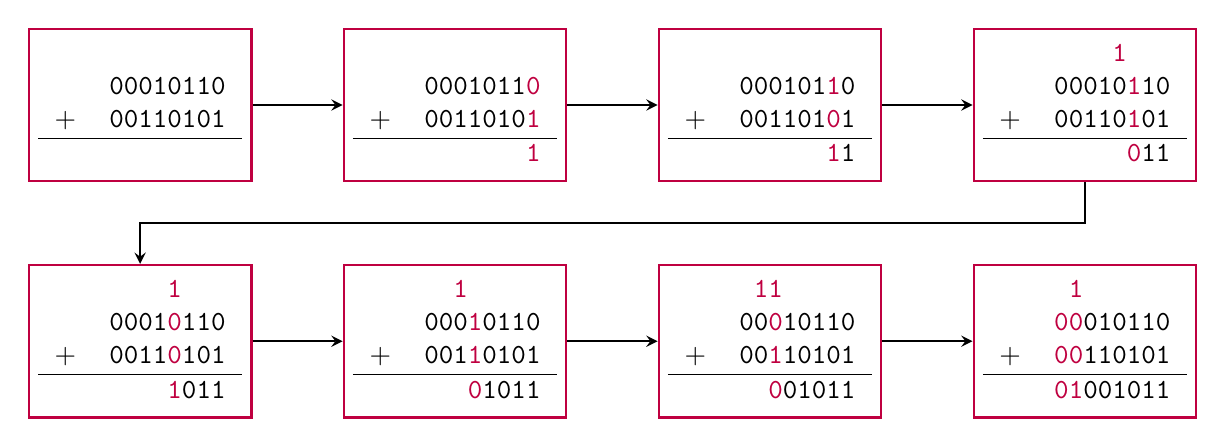
\begin{tikzpicture}[remember picture]
    \newcommand{\xStep}[0]{4cm}
    \newcommand{\yStep}[0]{3cm}
    \newcommand{\highl}[1]{\textcolor{purple}{#1}}
    \newcommand{\charspace}[0]{\textcolor{white}{0}}
    
    \tikzstyle{dedge} = [thick,->,>=stealth,draw=black]
    
    \tikzstyle{node}=[
      rectangle,
      draw=purple,
      anchor=center,
      thick,
      minimum size=1,
    ]
    
    \node[node] (n1) at (0*\xStep,0*\yStep) {
      \begin{tabular}{lr}
          & \texttt{} \\
          & \texttt{00010110} \\
        + & \texttt{00110101} \\
        \hline
          & \texttt{} \\
      \end{tabular}
    };
    
    \node[node] (n2) at (1*\xStep,0*\yStep) {
      \begin{tabular}{lr}
          & \texttt{} \\
          & \texttt{0001011\highl{0}} \\
        + & \texttt{0011010\highl{1}} \\
        \hline
          & \texttt{\highl{1}} \\
      \end{tabular}
    };
    
    \node[node] (n3) at (2*\xStep,0*\yStep) {
      \begin{tabular}{lr}
          & \texttt{} \\
          & \texttt{000101\highl{1}0} \\
        + & \texttt{001101\highl{0}1} \\
        \hline
          & \texttt{\highl{1}1} \\
      \end{tabular}
    };
    
    \node[node] (n4) at (3*\xStep,0*\yStep) {
      \begin{tabular}{lr}
          & \texttt{\highl{1}\charspace\charspace\charspace} \\
          & \texttt{00010\highl{1}10} \\
        + & \texttt{00110\highl{1}01} \\
        \hline
          & \texttt{\highl{0}11} \\
      \end{tabular}
    };
    
    \node[node] (n5) at (0*\xStep,-1*\yStep) {
      \begin{tabular}{lr}
          & \texttt{\highl{1}\charspace\charspace\charspace} \\
          & \texttt{0001\highl{0}110} \\
        + & \texttt{0011\highl{0}101} \\
        \hline
          & \texttt{\highl{1}011} \\
      \end{tabular}
    };
    
    \node[node] (n6) at (1*\xStep,-1*\yStep) {
      \begin{tabular}{lr}
          & \texttt{\highl{1}\charspace\charspace\charspace\charspace\charspace} \\
          & \texttt{000\highl{1}0110} \\
        + & \texttt{001\highl{1}0101} \\
        \hline
          & \texttt{\highl{0}1011} \\
      \end{tabular}
    };
    
    \node[node] (n7) at (2*\xStep,-1*\yStep) {
      \begin{tabular}{lr}
          & \texttt{\highl{1}\highl{1}\charspace\charspace\charspace\charspace\charspace} \\
          & \texttt{00\highl{0}10110} \\
        + & \texttt{00\highl{1}10101} \\
        \hline
          & \texttt{\highl{0}01011} \\
      \end{tabular}
    };
    
    \node[node] (n8) at (3*\xStep,-1*\yStep) {
      \begin{tabular}{lr}
          & \texttt{\highl{1}\charspace\charspace\charspace\charspace\charspace\charspace} \\
          & \texttt{\highl{00}010110} \\
        + & \texttt{\highl{00}110101} \\
        \hline
          & \texttt{\highl{01}001011} \\
      \end{tabular}
    };
    
    \draw[dedge] (n1)--(n2);
    \draw[dedge] (n2)--(n3);
    \draw[dedge] (n3)--(n4);
    \draw[dedge] (n4)|-(1.5*\xStep,-0.5*\yStep)-|(n5);
    \draw[dedge] (n5)--(n6);
    \draw[dedge] (n6)--(n7);
    \draw[dedge] (n7)--(n8);
  \end{tikzpicture}
\end{center}

  \caption{Addition of two 8-bit binary numbers.}
  \label{fig:prim:int:binary:add}
\end{figure}

% signedness: two's compliment

\csharpsubsection{\csharp}

% integer types available: and how to pick
\csharp\ supports the signed and unsigned integer types listed in figure \ref{fig:prim:int:csharp:types}. Lets say that you need to be able to represent any positive number below 100.000. That number sits somewhere in between the limits of 16 bits and 32 bits. This means that we need at least 32 bits, and if we use more than 32 bits to represent it then we will be wasting memory. Depending on our \idx{architecture}{Architecture!Processor}, there might be processing speed to \idx{trade}{Tradeoff} for this \say{wasted} memory. But lets just stick to the 32 bits for now. As we don't need the negative values we will go for an \typename{int}.

\begin{figure}[tbp]
  \begin{center}
  \begin{tabular}{rccl}
    \emph{Size} & \emph{Unsigned Type} & \emph{Signed Type} & \emph{Comment} \\
     8 bits & \typename{byte} & \typename{sbyte} & \\
    16 bits & \typename{ushort} & \typename{short} & \\
    32 bits & \typename{uint} & \typename{int} & \\
    64 bits & \typename{ulong} & \typename{long} & \\
    1 word & \typename{nuint} & \typename{nint} & Do not use\\
  \end{tabular}
\end{center}

  \caption{Integer types available in \csharp.}
  \label{fig:prim:int:csharp:types}
\end{figure}

% native types
That last line on the table is a little bit different though. You may have noticed that it is measured in \idx{words}{Word} instead of bits or bytes. On most processor architectures, a word will be defined as either 32 bits or 64 bits. See it as the most efficient integer size. The \typename{n} in \typename{nuint} and \typename{nint} stands for \textsl{\idx{native}{Native}}. A side-effect of using these types is that the effective MAXINT is machine dependent, and that can cause \idx{portability}{Portability} issues if you are not careful. For now, just stay away from these two types.

% naming conventions
The naming convention of the integer types is a bit unfortunate from a consistency perspective. The \typename{u} prefix is used to denote an \idx{unsigned}{Unsigned} variant, except for the \typename{byte} case where the \typename{s} prefix is used to denote an \idx{signed}{Signed} variant. In \typename{nuint} the \typename{u} still denotes something that is unsigned but it is not at the beginning of the name. So, from a human side, parsing these names if a relatively complex task. With a bit of experience though, you won't notice.

% what is the result of int32+int32? what is an overflow? %TODO: this was written higher up. Is that okay?

\begin{syntaxfloat}
  \begin{syntax}{expr}
  \SyntaxWestSplit{MainWest}
  \SyntaxEastSplit{MainEast}
  
  \node[nonterminal] (ruleIa)  at \SyntaxDistribute{MainWest}{MainEast}{1}{3} {expr};
  \node[terminal]    (ruleIb)  at \SyntaxDistribute{MainWest}{MainEast}{2}{3} {+};
  \node[nonterminal] (ruleIc)  at \SyntaxDistribute{MainWest}{MainEast}{3}{3} {expr};
  \node[nonterminal] (ruleIIa) at \SyntaxDistributeLine{MainWest}{MainEast}{1}{3}{1} {expr};
  \node[terminal]    (ruleIIb) at \SyntaxDistributeLine{MainWest}{MainEast}{2}{3}{1} {-};
  \node[nonterminal] (ruleIIc) at \SyntaxDistributeLine{MainWest}{MainEast}{3}{3}{1} {expr};
  \node[nonterminal] (ruleIIIa) at \SyntaxDistributeLine{MainWest}{MainEast}{1}{3}{2} {expr};
  \node[terminal]    (ruleIIIb) at \SyntaxDistributeLine{MainWest}{MainEast}{2}{3}{2} {*};
  \node[nonterminal] (ruleIIIc) at \SyntaxDistributeLine{MainWest}{MainEast}{3}{3}{2} {expr};
  \node[nonterminal] (ruleIVa) at \SyntaxDistributeLine{MainWest}{MainEast}{1}{3}{3} {expr};
  \node[terminal]    (ruleIVb) at \SyntaxDistributeLine{MainWest}{MainEast}{2}{3}{3} {/};
  \node[nonterminal] (ruleIVc) at \SyntaxDistributeLine{MainWest}{MainEast}{3}{3}{3} {expr};
  \node[nonterminal] (ruleVa) at \SyntaxDistributeLine{MainWest}{MainEast}{1}{3}{4} {expr};
  \node[terminal]    (ruleVb) at \SyntaxDistributeLine{MainWest}{MainEast}{2}{3}{4} {\%};
  \node[nonterminal] (ruleVc) at \SyntaxDistributeLine{MainWest}{MainEast}{3}{3}{4} {expr};
  
  \draw[path] (begin)--(ruleIa)--(ruleIb)--(ruleIc)--(end);
  \draw[path] (begin) to[-|-] (ruleIIa)--(ruleIIb)--(ruleIIc) to[-|-] (end);
  \draw[path] (begin) to[-|-] (ruleIIIa)--(ruleIIIb)--(ruleIIIc) to[-|-] (end);
  \draw[path] (begin) to[-|-] (ruleIVa)--(ruleIVb)--(ruleIVc) to[-|-] (end);
  \draw[path] (begin) to[-|-] (ruleVa)--(ruleVb)--(ruleVc) to[-|-] (end);
\end{syntax}

  \caption{Expressions of arithmetic operators}
  \label{syntax:prim:arithmetic:ops}
\end{syntaxfloat}

\elixirsubsection{Elixir}

% arbitrary sizes: pros
In Elixir, there is only one integer type and that has an \idx{arbitrary size}{Arbitrary size}. As long as an integral value fits in memory, an Elixir integer can hold it. The value is not in having integers that each take up 90\% of your \idx{primary memory}{Memory!Primary}. It is very rare that we have a need for integers beyond 128 bits or even 64 bits. But when we work with \idx{fixed size}{Fixed size} integers, we always have to be aware of that hard limit. In Elixir, we don't have to: If we somehow end up with a number needing 7000 bits, then that is what gets allocated. We don't have to worry.

% and cons, why the tradeoff was resolved in this way
Elixir code, still runs on the same hardware though. This hardware does not have instructions capable of operating on 7000 bit integers. So, instead of an integer operation being a single \idx{instruction}{Instruction}, it is an \idx{algorithm}{Algorithm} in itself. This is significantly slower. Elixir is designed for network intensive tasks, and these are even slower. So, for the tasks where one would choose Elixir, it basically doesn't matter. And that is why the designers of that language has made that choice.

\section{Floating Point Numbers}
\label{primitives:float}

\subsection{Operations}
\subsection{Representation}
\csharpsubsection{\csharp}
\elixirsubsection{Elixir}

\section{Truth Values}
\label{primitives:bools}

% what do they represent

\subsection{Operations on Nontruthy Values}

Any valid comparison between two nontruthy values will yield a truthy value. For instance, if we ask \quoted{is 42 equal to 56?} then the resulting value is \valuename{false} but if we ask \quoted{is 1 less than or equal to 2?} then the resulting value is \valuename{true}. The full set of comparison operators are listed in figure \ref{fig:prim:bool:comparison}. This is one of the primary ways of creating boolean values.

\begin{figure}[tbp]
  \begin{center}
  \begin{tabular}{cl}
    $a$ \texttt{==} $b$ & True if $a$ is the same as $b$ \\
    $a$ \texttt{!=} $b$ & True if $a$ is different from $b$ \\
    $a$ \texttt{<} $b$ & True if $a$ is less than $b$ \\
    $a$ \texttt{<=} $b$ & True if $a$ is less than or equal to $b$ \\
    $a$ \texttt{>} $b$ & True if $a$ is greater than $b$ \\
    $a$ \texttt{>=} $b$ & True if $a$ is greater than or equal to $b$ \\
  \end{tabular}
\end{center}

  \caption{Comparison operators.}
  \label{fig:prim:bool:comparison}
\end{figure}

\subsection{Operations on Truth Values}

\begin{figure}[tbp]
  \begin{center}
  \begin{tabular}{cccccc}
    $a$ & $b$ & $a \wedge b$ & $a \vee b$ & $a \oplus b$ & $\neg a$\\
    0 & 0 & 0 & 0 & 0 & 1 \\
    0 & 1 & 0 & 1 & 1 & \\
    1 & 0 & 0 & 1 & 1 & 0 \\
    1 & 1 & 1 & 1 & 0 & \\
  \end{tabular}
\end{center}

  \caption{Truth table for the boolean operations.}
  \label{fig:prim:bool:and}
\end{figure}

% TODO: De Morgan's law

\subsection{Representation}

% technically a bit, but typically (mostly unless in array form) a byte or word

\csharpsubsection{\csharp}

\begin{syntaxfloat}
  \begin{syntax}{expr}
  \SyntaxWestSplit{MainWest}
  \SyntaxEastSplit{MainEast}
  
  \node[sequence] () at ([yshift=0*\syntaxruledist]$(begin)!0.5!(end)$) {
    \node[nonterminal] (ruleIa) {expr};
    &
    \node[terminal]    (ruleIb) {\&\&};
    &
    \node[nonterminal] (ruleIc) {expr};
    \\
  };
  
  \node[sequence] () at ([yshift=-1*\syntaxruledist]$(begin)!0.5!(end)$) {
    \node[nonterminal] (ruleIIa) {expr};
    &
    \node[terminal]    (ruleIIb) {||};
    &
    \node[nonterminal] (ruleIIc) {expr};
    \\
  };
  
  \node[sequence] () at ([yshift=-2*\syntaxruledist]$(begin)!0.5!(end)$) {
    \node[nonterminal] (ruleIIIa) {expr};
    &
    \node[terminal]    (ruleIIIb) {\^{}};
    &
    \node[nonterminal] (ruleIIIc) {expr};
    \\
  };
  
  \node[sequence] () at ([yshift=-3*\syntaxruledist]$(begin)!0.5!(end)$) {
    \node[terminal]    (ruleIVa) {!};
    &
    \node[nonterminal] (ruleIVb) {expr};
    \\
  };
  
  \draw[path] (begin)--(ruleIa)--(ruleIb)--(ruleIc)--(end);
  \draw[path] (begin) to[-|-] ([xshift=4cm,yshift=-1*\syntaxruledist]begin.east)--(ruleIIa)--(ruleIIb)--(ruleIIc)--([xshift=-4cm,yshift=-1*\syntaxruledist]end.west) to[-|-] (end);
  \draw[path] (begin) to[-|-] ([xshift=4cm,yshift=-2*\syntaxruledist]begin.east)--(ruleIIIa)--(ruleIIIb)--(ruleIIIc)--([xshift=-4cm,yshift=-2*\syntaxruledist]end.west) to[-|-] (end);
  \draw[path] (begin) to[-|-] ([xshift=4cm,yshift=-3*\syntaxruledist]begin.east)--(ruleIVa)--(ruleIVb)--([xshift=-4cm,yshift=-3*\syntaxruledist]end.west) to[-|-] (end);
\end{syntax}

  \caption{Expressions of boolean operators}
  \label{syntax:prim:bool:ops}
\end{syntaxfloat}

\elixirsubsection{Elixir}

\csubsection{C}

% low-level language
\idx{C}{Language!C} is a simple \idx{low-level language}{Language!Low-level}. That means that it mirrors the fundamental properties of the underlying harware and adds some highly convenient abstractions. These abstractions are chosen is such a way that they essentially can be delivered without a performance overhead.

% consequence: a boolean is a register
\idxx{Machine code} does not have a boolean type. Instead \idx{register}{Register} values that are represented using all zeroes in binary are \textsl{false} and every other value is \textsl{true}. That means -- in terms of integers -- that zero is \textsl{false} and non-zero is \textsl{true}. % TODO: Explain the !!42 == 1 situation, word for reference/strong true values, implicit konvertering til bool i condition af en if

% consequence: a bool is an integer and can thus be used in an integer expression
A consequence of this is that C doesn't have a notion of a \idx{boolean}{Boolean}. Instead, integers are used: A boolean is an interpretation of an integer, and can thus be used in an integer expression. Typically, this will make absolutely no difference. Proponents of \csharp\ will point out that booleans and integers are fundamentally different notions and should thus be treated differently. Proponents of C will point out that this allows them to write code such as this:

% TODO: Example

% explanation: why is this clever (no branches gives execution speed, and it is still readable)

\section{Local Variables}
\csharpsubsection{\csharp}

\begin{syntaxfloat}
  \begin{syntax}[[xshift=22mm]concept.west]{type}
  \SyntaxWestSplit{MainWest}
  \SyntaxEastSplit{MainEast}
  
  \node[terminal] (ruleIa) at ($(begin)!0.5!(end)$) {name};
  
  \draw[path] (begin)--(ruleIa)--(end);
\end{syntax}
\begin{syntax}[[xshift=22mm]concept.west]{local-var}
  \SyntaxWestSplit{MainWest}
  \SyntaxEastSplit{MainEast}
  
  \node[sequence,anchor=north] () at ([yshift=\syntaxrulenodeheight-0.8pt*3]$(begin.east)!0.5!(end.west)$) {
    \node[nonterminal] (ruleIa) {type};
    &
    \node[terminal]    (ruleIb) {name};
    &
    \node[terminal]    (ruleIc) {=};
    &
    \node[nonterminal] (ruleId) {expr};
    &
    \node[terminal]    (ruleIe) {;};
    \\
    \node[nonterminal] (ruleIIa) {type};
    &
    \node[terminal]    (ruleIIb) {name};
    &
    &
    &
    \node[terminal]    (ruleIIc) {;};
    \\
  };
  
  \draw[path] (begin)--(ruleIa)--(ruleIb)--(ruleIc)--(ruleId)--(ruleIe)--(end);
  \draw[path] (begin) to[-|-] ([xshift=2cm,yshift=-1*(\syntaxruledist+0.8pt*3)]begin.east)--(ruleIIa)--(ruleIIb)--(ruleIIc)--([xshift=-2cm,yshift=-1*(\syntaxruledist+0.8pt*3)]end.west) to[-|-] (end);
\end{syntax}
\begin{syntax}[[xshift=22mm]concept.west]{stmt}
  \SyntaxWestSplit{MainWest}
  \SyntaxEastSplit{MainEast}
  
  \node[nonterminal] (ruleIa) at ($(begin)!0.5!(end)$) {local-var};
  
  \draw[path] (begin)--(ruleIa)--(end);
\end{syntax}


  \caption{Local variables.}
  \label{syntax:prim:vars:locals}
\end{syntaxfloat}

\elixirsubsection{Elixir}

\section{Parsing}
\subsection{Operator Precedence}

% parentheses

\subsection{Operator Associativity}

\csharpsubsection{\csharp}

\begin{syntaxfloat}
  \begin{syntax}{expr}
  \SyntaxWestSplit{MainWest}
  \SyntaxEastSplit{MainEast}
  
  \node[sequence] () at ([yshift=0*\syntaxruledist]$(begin)!0.5!(end)$) {
    \node[terminal]    (ruleIa) {(};
    &
    \node[nonterminal] (ruleIb) {expr};
    &
    \node[terminal]    (ruleIc) {)};
    \\
  };
  
  \draw[path] (begin)--(ruleIa)--(ruleIb)--(ruleIc)--(end);
\end{syntax}

  \caption{Expressions of parentheses}
  \label{syntax:prim:pars}
\end{syntaxfloat}

\exercises{primitives}{Primitive Types}


\chapter{Flow Control}

\section{Choices in Logic}
\label{sec:flow:branch}

% motivation

\subsection{\keywordname{if} and \keywordname{else}}

\subsection{Blocks}

\subsection{\keywordname{unless}}

\subsection{Chaining Branches}

% common pattern: define pattern

\elixirsubsubsection{Elixir}

\csharpsubsubsection{\csharp}

\subsection{\keywordname{switch} and \keywordname{case}}

\csharpsubsection{\csharp}

\begin{syntaxfloat}
  \section{Choices in Logic}
\label{sec:flow:branch}

% motivation

\subsection{\keywordname{if} and \keywordname{else}}

\subsection{Blocks}

\subsection{\keywordname{unless}}

\subsection{Chaining Branches}

% common pattern: define pattern

\elixirsubsubsection{Elixir}

\csharpsubsubsection{\csharp}

\subsection{\keywordname{switch} and \keywordname{case}}

\csharpsubsection{\csharp}

\begin{syntaxfloat}
  \input{syntax/flow_branch.tex}
  \caption{Statements for branching}
  \label{syntax:flow:branch}
\end{syntaxfloat}

\elixirsubsection{Elixir}


\subsection{Blocks}

% problem motivating the need

\subsubsection{Dangling Else}
\label{sec:flow:branch:danglingelse}

% problem: take a moment to look at CODE, do a manual execution of it, and note down what the result was.

% parse trees: as we know the compiler sees the code differently from humans, it converts it into a sequence of tokens and then builds a parse tree from it, one can easily imagine two possible outcomes of this as illustrated in figure FIG

% figure of the two parse trees

% however, the rules that govern how the parse tree is constructed dictates that it is the version to the right is the correct variant, why?

% problem & solution: The problem here is that the indentations were \say{wrong}, and that likely fooled you, two mistakes were made (wrong indent, relying on indent for understanding), both are very easy to make, the way around this is to always use blocks to disambiguate

% solution example

\csharpsubsection{\csharp}

\begin{syntaxfloat}
  \input{syntax/flow_block.tex}
  \caption{Block statements}
  \label{syntax:flow:block}
\end{syntaxfloat}


  \caption{Statements for branching}
  \label{syntax:flow:branch}
\end{syntaxfloat}

\elixirsubsection{Elixir}


\subsection{Blocks}

% problem motivating the need

\subsubsection{Dangling Else}
\label{sec:flow:branch:danglingelse}

% problem: take a moment to look at CODE, do a manual execution of it, and note down what the result was.

% parse trees: as we know the compiler sees the code differently from humans, it converts it into a sequence of tokens and then builds a parse tree from it, one can easily imagine two possible outcomes of this as illustrated in figure FIG

% figure of the two parse trees

% however, the rules that govern how the parse tree is constructed dictates that it is the version to the right is the correct variant, why?

% problem & solution: The problem here is that the indentations were \say{wrong}, and that likely fooled you, two mistakes were made (wrong indent, relying on indent for understanding), both are very easy to make, the way around this is to always use blocks to disambiguate

% solution example

\csharpsubsection{\csharp}

\begin{syntaxfloat}
  \begin{syntax}{stmt}
  \SyntaxWestSplit{MainWest}
  \SyntaxEastSplit{MainEast}
  
  \node[sequence] () at ([yshift=0*\syntaxruledist]$(begin)!0.5!(end)$) {
    \node[terminal]    (ruleIa) {\{};
    &
    \node[nonterminal] (ruleIb) {stmts};
    &
    \node[terminal]    (ruleIc) {\}};
    \\
  };
  
  \draw[path] (begin)--(ruleIa)--(ruleIb)--(ruleIc)--(end);
\end{syntax}

  \caption{Block statements}
  \label{syntax:flow:block}
\end{syntaxfloat}


\section{Repetition}
\label{sec:flow:repetition}

% problem: print something once, twice, 1000 times, scalability problem, variable number of times

\begin{syntaxfloat}
  \section{Repetition}
\label{sec:flow:repetition}

% problem: print something once, twice, 1000 times, scalability problem, variable number of times

\begin{syntaxfloat}
  \input{syntax/flow_repetition.tex}
  \caption{Statements for repetition}
  \label{syntax:flow:repetition}
\end{syntaxfloat}

\subsection{\keywordname{while}}

% highlevel concept: speaking alout explanation

% figure: flowchart

\subsection{\keywordname{do-while}}

% highlevel concept: speaking alout explanation

% figure: flowchart

\subsection{Converting Between \keywordname{while} and \keywordname{do-while}}

% intro: one can convert one to the other

% figure: subfigure for each direction

% which option to go for? problem of repetion

\subsection{\keywordname{for}}


  \caption{Statements for repetition}
  \label{syntax:flow:repetition}
\end{syntaxfloat}

\subsection{\keywordname{while}}

% highlevel concept: speaking alout explanation

% figure: flowchart

\subsection{\keywordname{do-while}}

% highlevel concept: speaking alout explanation

% figure: flowchart

\subsection{Converting Between \keywordname{while} and \keywordname{do-while}}

% intro: one can convert one to the other

% figure: subfigure for each direction

% which option to go for? problem of repetion

\subsection{\keywordname{for}}



\exercises{flow}{Flow Control}

\chapter{Basic Datastructures}

% the problem of working with individual values

\section{Types}

\subsection{Complex Types}

\subsection{Reference Types}

\section{Structured Data}

\subsection{Colors}

% light as a spectrum
\defix{Light} is made up of photons, and each \idx{photon}{Photon} has a wavelength. The \defi{wavelength}{Wavelength} of the photons determines which color our eyes will observe. A wavelength of 380nm is \idx{violet}{Violet} and one of 740nm is \idx{red}{Red}. In between these you have all the colors of the \idx{rainbow}{Rainbow}, in the order of the rainbow. Coincidence? Just outside of the \idx{visible spectrum}{Spectrum!Visible}, you will find \idx{infra-red}{Infra-red} and \idx{ultra-violet}{Untra-violet}. Our eyes are, however, constantly bombarded by photons, so in reality we always observe a distribution across this spectrum. Our \idx{eyes}{Eye}, though only has three (or four) tunings of receptors. These, roughly corresponds to red, green and blue. So, your eyes (and \idx{brains}{Brain}) need to do a lot of interpretation.

% computer representation
In a computer, colors are typically \idx{represented}{Representation!Color} using three values; one for red intensity, one for green intensity, and one for blue intensity. That somehow matches the model of our eyes \ldots We say that these are the \textsl{components} of the color. There is a number of ways to express such an \idx{intensity}{Intensity}. It seem natural to use a number between 0 and 100, or perhaps a number between 0.0 and 1.0. However, due to the way processors work on integers, these boundaries are not particularly special. Typically, a byte is use to represent each component of the color. That means that we have the ability to express $2^8=256$ different intensities of each component, or a total of $256^3=16777216$ different colors. The value zero is used to represent complete \idx{darkness}{Darkness}. Full intensity is then the value 255.

% figure: color cube
\begin{figure}[tbp]
  \begin{center}
  \scalebox{1.0}{
    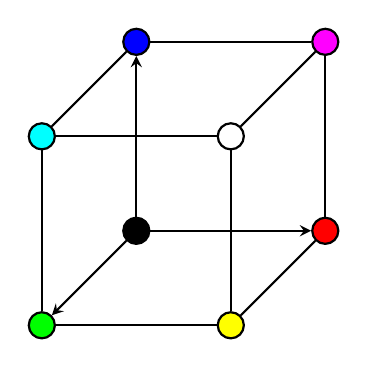
\begin{tikzpicture}
      \newcommand{\dist}[0]{24mm}
      \newcommand{\zdist}[0]{12mm}
      
      \tikzstyle{node}=[
        draw,
        circle,
        minimum height=0.2cm,
        minimum width=0.2cm,
        anchor=center,
        thick
      ]
      \tikzstyle{arrow} = [thick,->,>=stealth, draw=black]
      \tikzstyle{line} = [thick, draw=black]
      
      \definecolor{mycyan}{rgb}{0.0,1.0,1.0}
      \definecolor{mymagenta}{rgb}{1.0,0.0,1.0}
      \definecolor{myyellow}{rgb}{1.0,1.0,0.0}
      
      \node[node, fill=blue]      (blue)    at (0    , 0) {};
      \node[node, fill=mymagenta] (magenta) at (\dist, 0) {};
      \node[node, fill=black]     (black)   at (0    , -\dist) {};
      \node[node, fill=red]       (red)     at (\dist, -\dist) {};
      \node[node, fill=mycyan]   (cyan)   at (0-\zdist    , 0-\zdist) {};
      \node[node, fill=white]    (white)  at (\dist-\zdist, 0-\zdist) {};
      \node[node, fill=green]    (green)  at (0-\zdist    , -\dist-\zdist) {};
      \node[node, fill=myyellow] (yellow) at (\dist-\zdist, -\dist-\zdist) {};
      
      \draw[arrow] (black) -- (red);
      \draw[arrow] (black) -- (green);
      \draw[arrow] (black) -- (blue);
      \draw[line] (blue) -- (magenta);
      \draw[line] (blue) -- (cyan);
      \draw[line] (red) -- (magenta);
      \draw[line] (red) -- (yellow);
      \draw[line] (green) -- (yellow);
      \draw[line] (green) -- (cyan);
      \draw[line] (white) -- (cyan);
      \draw[line] (white) -- (magenta);
      \draw[line] (white) -- (yellow);
    \end{tikzpicture}
  }
\end{center}

  \caption{RGB color cube.}
  \label{fig:primdata:struct:color}
\end{figure}

% color spaces
This constitutes a \defi{color space}{Color!Space} whereby all colors fit within a \idx{color cube}{Color!Cube} spanned by the red, green and blue color vectors. Hence, it is named the \idxx{RGB} color space. Figure \ref{fig:primdata:struct:color} depicts this space. It is a direct fit for how \idx{GPUs}{GPU} represent \idx{images}{Image}. Other color spaces exist though, and there are good reasons for their existence. Other popular color spaces include \idxx{HSV} (which is shaped like a cylinder) and \idxx{XYZ} (which is shaped like an tongue). Formulas exists for \idx{converting}{Color!Space!Converting} between these. Each of these color spaces represents practical simplifications of what light really is.

\csharpsubsection{\csharp}

% value type through struct, reference type through class

\begin{syntaxfloat}
  \begin{syntax}[[xshift=22mm]concept.west]{vismod}
  \SyntaxWestSplit{MainWest}
  \SyntaxEastSplit{MainEast}
  
  \node[terminal] (ruleIa) at ($(begin)!0.5!(end)$) {public};
  
  \draw[path] (begin)--(ruleIa)--(end);
\end{syntax}

\begin{syntax}[[xshift=22mm]concept.west]{global-var}
  \SyntaxWestSplit{MainWest}
  \SyntaxEastSplit{MainEast}
  
  \node[sequence,anchor=north] () at ([yshift=\syntaxrulenodeheight-0.8pt*3]$(begin.east)!0.5!(end.west)$) {
    \node[nonterminal] (ruleIa) {vismod};
    &
    \node[nonterminal] (ruleIb) {type};
    &
    \node[terminal]    (ruleIc) {name};
    &
    \node[terminal]    (ruleId) {=};
    &
    \node[nonterminal] (ruleIe) {expr};
    &
    \node[terminal]    (ruleIf) {;};
    \\
    \node[nonterminal] (ruleIIa) {vismod};
    &
    \node[nonterminal] (ruleIIb) {type};
    &
    \node[terminal]    (ruleIIc) {name};
    &
    &
    &
    \node[terminal]    (ruleIId) {;};
    \\
  };
  
  \draw[path] (begin)--(ruleIa)--(ruleIb)--(ruleIc)--(ruleId)--(ruleIe)--(ruleIf)--(end);
  \draw[path] (begin) to[-|-] ([xshift=1cm,yshift=-1*(\syntaxruledist+0.8pt*3)]begin.east)--(ruleIIa)--(ruleIIb)--(ruleIIc)--(ruleIId)--([xshift=-1cm,yshift=-1*(\syntaxruledist+0.8pt*3)]end.west) to[-|-] (end);
\end{syntax}

\begin{syntax}[[xshift=24mm]concept.west]{global-vars}
  \SyntaxWestSplit{MainWest}
  \SyntaxEastSplit{MainEast}
  
  \node[sequence] () at ([yshift=\syntaxruledist-0.8pt*3]$(begin)!0.5!(end)$) {
    \\
    \node[nonterminal]    (ruleIa) {global-var};
    \\
  };
  
  \draw[path] (begin)--(end);
  \draw[path] (begin) to[-|-] (ruleIa) to[-|-] (end);
  \draw[path] (ruleIa)
            -|([xshift= 0.5*\syntaxruledist,yshift=0.4*\syntaxruledist]ruleIa.east)
            |-(                            [yshift=0.8*\syntaxruledist]ruleIa.center)
            -|([xshift=-0.5*\syntaxruledist,yshift=0.4*\syntaxruledist]ruleIa.west)
            |-(ruleIa);
\end{syntax}

\begin{syntax}[[xshift=22mm]concept.west]{class}
  \SyntaxWestSplit{MainWest}
  \SyntaxEastSplit{MainEast}
  
  \node[sequence,anchor=north] () at ([yshift=\syntaxrulenodeheight-0.8pt*3]$(begin.east)!0.5!(end.west)$) {
    \node[terminal]    (ruleIa) {class};
    &
    \node[terminal]    (ruleIb) {name};
    &
    \node[terminal]    (ruleIc) {\{};
    &
    \node[nonterminal] (ruleId) {global-vars};
    &
    \node[terminal]    (ruleIe) {\}};
    \\
  };
  
  \draw[path] (begin)--(ruleIa)--(ruleIb)--(ruleIc)--(ruleId)--(ruleIe)--(end);
\end{syntax}

  \caption{Structured data}
  \label{syntax:data:struct}
\end{syntaxfloat}

\section{Sequences in Data}

\subsection{Arrays}

\subsubsection{Indexing}

% calculation, this is why most languages agree that arrays start at zero

\subsubsection{Multidimensional Arrays}

\subsection{Linked Lists}

% head and tail

\subsection{Doubly Linked Lists}

\subsection{Looping Sequences}

\subsection{Nesting}

\subsection{Points}

\section{Enumerations}

\subsection{State Machines}

\subsection{String Parsing Example}

\section{Case: Dynamic Arrays} % TODO: should this go into the function chapter?

% problem: arrays have a static size

% observation: a variable only references an array

% solution: Wrap the array in a struct

\csharpsubsection{\csharp}

\begin{syntaxfloat}
  \begin{syntax}[[xshift=24mm]concept.west]{names}
  \SyntaxWestSplit{MainWest}
  \SyntaxEastSplit{MainEast}
  
  \node[sequence] () at ([yshift=-0*\syntaxruledist]$(begin)!0.5!(end)$) {
    \node[nonterminal]    (ruleIa) {name};
    \\
  };
  
  \node[sequence] () at ([yshift=1*\syntaxruledist]$(begin)!0.5!(end)$) {
    \node[terminal]    (ruleIIa) {,};
    \\
  };
  
  \draw[path] (begin)--(ruleIa)--(end);
  \draw[path] (ruleIa)
            -|([xshift= 0.5*\syntaxruledist,yshift=0.4*\syntaxruledist]ruleIa.east)
            |-(                            [yshift=0.0*\syntaxruledist]ruleIIa)
            -|([xshift=-0.5*\syntaxruledist,yshift=0.4*\syntaxruledist]ruleIa.west)
            |-(ruleIa);
\end{syntax}

\begin{syntax}[[xshift=22mm]concept.west]{enum}
  \SyntaxWestSplit{MainWest}
  \SyntaxEastSplit{MainEast}
  
  \node[sequence,anchor=north] () at ([yshift=\syntaxrulenodeheight-0.8pt*3]$(begin.east)!0.5!(end.west)$) {
    \node[terminal]    (ruleIa) {enum};
    &
    \node[terminal]    (ruleIb) {name};
    &
    \node[terminal]    (ruleIc) {\{};
    &
    \node[nonterminal] (ruleId) {names};
    &
    \node[terminal]    (ruleIe) {\}};
    \\
  };
  
  \draw[path] (begin)--(ruleIa)--(ruleIb)--(ruleIc)--(ruleId)--(ruleIe)--(end);
\end{syntax}

  \caption{Enums}
  \label{syntax:data:enum}
\end{syntaxfloat}


\chapter{Code Reuse}

Hello

\section{Mathematical Functions}

\section{Concrete Implementations}

\csharpsubsection{\csharp}

\begin{syntaxfloat}
  \begin{syntax}[[xshift=22mm]concept.west]{params}
  \SyntaxWestSplit{MainWest}
  \SyntaxEastSplit{MainEast}
  
  \node[sequence,column sep=1.5cm] () at ([yshift=-0*\syntaxruledist]$(begin)!0.5!(end)$) {
    \node[nonterminal] (ruleIa) {type};
    &
    \node[terminal]    (ruleIb) {name};
    \\
  };
  
  \node[sequence,column sep=1.0cm] () at ([yshift=1*\syntaxruledist]$(ruleIa)!0.5!(ruleIb)$) {
    \node[terminal]    (ruleIIa) {,};
    \\
  };
  
  \draw[path] (begin)--(ruleIa)--(ruleIb)--(end);
  \draw[path] (ruleIb)
            -|([xshift= 0.75*\syntaxruledist,yshift=0.4*\syntaxruledist]ruleIb.east)
            |-(                            [yshift=0.0*\syntaxruledist]ruleIIa)
            -|([xshift=-0.75*\syntaxruledist,yshift=0.4*\syntaxruledist]ruleIa.west)
            |-(ruleIa);
\end{syntax}

\begin{syntax}[[xshift=22mm]concept.west]{fun-def}
  \SyntaxWestSplit{MainWest}
  \SyntaxEastSplit{MainEast}
  
  \node[sequence,column sep=1.2cm] () at ([yshift=-0*\syntaxruledist]$(begin)!0.5!(end)$) {
    \node[nonterminal] (ruleIa) {type};
    &
    \node[terminal]    (ruleIb) {name};
    &
    \node[terminal]    (ruleIc) {(};
    &
    \node[nonterminal] (ruleId) {params};
    &
    \node[terminal]    (ruleIe) {)};
    &
    \node[terminal]    (ruleIf) {stmt};
    \\
  };
  
  \draw[path] (begin)--(ruleIa)--(ruleIb)--(ruleIc)--(ruleId)--(ruleIe)--(ruleIf)--(end);
\end{syntax}
\begin{syntax}[[xshift=22mm]concept.west]{args}
  \SyntaxWestSplit{MainWest}
  \SyntaxEastSplit{MainEast}
  
  \node[sequence,column sep=1.5cm] () at ([yshift=-0*\syntaxruledist]$(begin)!0.5!(end)$) {
    \node[nonterminal] (ruleIa) {expr};
    \\
  };
  
  \node[sequence,column sep=1.0cm] () at ([yshift=1*\syntaxruledist]ruleIa) {
    \node[terminal]    (ruleIIa) {,};
    \\
  };
  
  \draw[path] (begin)--(ruleIa)--(end);
  \draw[path] (ruleIa)
            -|([xshift= 0.75*\syntaxruledist,yshift=0.4*\syntaxruledist]ruleIa.east)
            |-(                            [yshift=0.0*\syntaxruledist]ruleIIa)
            -|([xshift=-0.75*\syntaxruledist,yshift=0.4*\syntaxruledist]ruleIa.west)
            |-(ruleIa);
  \draw[path] (begin)
            -|([xshift=-1.5*\syntaxruledist,yshift=-0.5*\syntaxruledist]ruleIa.west)
            |-(                            [yshift=-1.0*\syntaxruledist]ruleIa.center)
            -|([xshift= 1.5*\syntaxruledist,yshift=-0.5*\syntaxruledist]ruleIa.east)
            |-(end);
\end{syntax}

\begin{syntax}[[xshift=22mm]concept.west]{fun-call}
  \SyntaxWestSplit{MainWest}
  \SyntaxEastSplit{MainEast}
  
  \node[sequence,column sep=1.5cm] () at ([yshift=-0*\syntaxruledist]$(begin)!0.5!(end)$) {
    \node[terminal]    (ruleIa) {name};
    &
    \node[terminal]    (ruleIb) {(};
    &
    \node[nonterminal] (ruleIc) {args};
    &
    \node[terminal]    (ruleId) {)};
    \\
  };
  
  \draw[path] (begin)--(ruleIa)--(ruleIb)--(ruleIc)--(ruleId)--(end);
\end{syntax}

\begin{syntax}[[xshift=22mm]concept.west]{expr}
  \SyntaxWestSplit{MainWest}
  \SyntaxEastSplit{MainEast}
  
  \node[sequence,column sep=1.5cm] () at ([yshift=-0*\syntaxruledist]$(begin)!0.5!(end)$) {
    \node[nonterminal] (ruleIa) {fun-call};
    \\
  };
  
  \draw[path] (begin)--(ruleIa)--(end);
\end{syntax}

\begin{syntax}[[xshift=22mm]concept.west]{stmt}
  \SyntaxWestSplit{MainWest}
  \SyntaxEastSplit{MainEast}
  
  \node[sequence,column sep=1.5cm] () at ([yshift=-0*\syntaxruledist]$(begin)!0.5!(end)$) {
    \node[nonterminal] (ruleIa) {fun-def};
    \\
  };
  
  \node[sequence,column sep=1.5cm] () at ([yshift=-1*\syntaxruledist]$(begin)!0.5!(end)$) {
    \node[nonterminal] (ruleIIa) {fun-call};
    &
    \node[terminal]    (ruleIIb) {;};
    \\
  };
  
  \draw[path] (begin)--(ruleIa)--(end);
  \draw[path] (begin)
            -|([xshift=-1.5*\syntaxruledist,yshift=0.5*\syntaxruledist]ruleIIa.west)
            |-(                                                         ruleIIa)
            --(                                                         ruleIIb)
            -|([xshift= 1.5*\syntaxruledist,yshift=0.5*\syntaxruledist]ruleIIb.east)
            |-(end);
\end{syntax}


  \caption{Functions.}
  \label{syntax:fun}
\end{syntaxfloat}

% parameters vs arguments

% both as expressions and as statements

% nested functions

\pythonsubsection{Python}

\elixirsubsection{Elixir}

\exercises{functions}{Functions}

\chapter{Exceptions}

Hello


\begin{syntaxfloat}
  \begin{syntax}[[xshift=18mm]concept.west]{expr}
  \SyntaxWestSplit{MainWest}
  \SyntaxEastSplit{MainEast}
  
  \node[sequence,column sep=1.1cm] () at ([yshift=-0*\syntaxruledist]$(begin)!0.5!(end)$) {
    \node[terminal]    (ruleIa) {new};
    &
    \node[nonterminal] (ruleIb) {name};
    &
    \node[terminal]    (ruleIc) {(};
    &
    \node[nonterminal] (ruleId) {args};
    &
    \node[terminal]    (ruleIe) {)};
    \\
  };
  
  \draw[path] (begin)--(ruleIa)--(ruleIb)--(ruleIc)--(ruleId)--(ruleIe)--(end);
\end{syntax}

\begin{syntax}[[xshift=18mm]concept.west]{stmt}
  \SyntaxWestSplit{MainWest}
  \SyntaxEastSplit{MainEast}
  
  \node[sequence,column sep=2.0cm] () at ([yshift=-0*\syntaxruledist]$(begin)!0.5!(end)$) {
    \node[terminal]    (ruleIa) {throw};
    &
    \node[nonterminal] (ruleIb) {expr};
    &
    \node[terminal]    (ruleIc) {;};
    \\
  };
  
  \draw[path] (begin)--(ruleIa)--(ruleIb)--(ruleIc)--(end);
\end{syntax}

\begin{syntax}[[xshift=18mm]concept.west]{catch}
  \SyntaxWestSplit{MainWest}
  \SyntaxEastSplit{MainEast}
  
  \node[sequence,column sep=1.1cm] () at ([yshift=-0*\syntaxruledist]$(begin)!0.5!(end)$) {
    \node[terminal]    (ruleIa) {catch};
    &
    \node[terminal]    (ruleIb) {(};
    &
    \node[nonterminal] (ruleIc) {type};
    &
    \node[nonterminal] (ruleId) {name};
    &
    \node[terminal]    (ruleIe) {)};
    &
    \node[nonterminal] (ruleIf) {stmt};
    \\
  };
  
  \draw[path] (begin)--(ruleIa)--(ruleIb)--(ruleIc)--(ruleId)--(ruleIe)--(ruleIf)--(end);
  
  % bypass name
  \draw[path] (ruleIc)
            -|([xshift=-0.5*\syntaxruledist,yshift=0.4*\syntaxruledist]ruleId.west)
            |-([                             yshift=1.0*\syntaxruledist]ruleId.center)
            -|([xshift= 0.5*\syntaxruledist,yshift=0.4*\syntaxruledist]ruleId.east)
            |-(ruleIe);
\end{syntax}

\begin{syntax}[[xshift=18mm]concept.west]{finally}
  \SyntaxWestSplit{MainWest}
  \SyntaxEastSplit{MainEast}
  
  \node[sequence,column sep=2.0cm] () at ([yshift=-0*\syntaxruledist]$(begin)!0.5!(end)$) {
    \node[terminal]    (ruleIa) {finally};
    &
    \node[nonterminal] (ruleIb) {stmt};
    \\
  };
  
  \draw[path] (begin)--(ruleIa)--(ruleIb)--(end);
\end{syntax}

\begin{syntax}[[xshift=18mm]concept.west]{stmt}
  \SyntaxWestSplit{MainWest}
  \SyntaxEastSplit{MainEast}
  
  \node[sequence,column sep=2.0cm] () at ([yshift=-0*\syntaxruledist]$(begin)!0.5!(end)$) {
    \node[terminal]    (ruleIa) {try};
    &
    \node[nonterminal] (ruleIb) {catch};
    &
    \node[nonterminal] (ruleIc) {finally};
    \\
  };
  
  \node[sequence,column sep=2.0cm] () at ([yshift=-1*\syntaxruledist]$(begin)!0.5!(end)$) {
    \node[terminal]    (ruleIIa) {try};
    &
    \node[nonterminal] (ruleIIb) {catch};
    &
    \node[nonterminal] (ruleIIc) {finally};
    \\
  };
  
  \draw[path] (begin)--(ruleIa)--(ruleIb)--(ruleIc)--(end);
  
  \draw[path] (begin)
            -|([xshift=-0.75*\syntaxruledist,yshift=0.4*\syntaxruledist]ruleIIa.west)
            |-(ruleIIa)
            --(ruleIIb)
            --(ruleIIc)
            -|([xshift= 0.75*\syntaxruledist,yshift=0.4*\syntaxruledist]ruleIIc.east)
            |-(end);
  
  % loop upper catch
  \draw[path] (ruleIb)
            -|([xshift= 0.75*\syntaxruledist,yshift=0.4*\syntaxruledist]ruleIb.east)
            |-([                             yshift=1.0*\syntaxruledist]ruleIb.center)
            -|([xshift=-0.75*\syntaxruledist,yshift=0.4*\syntaxruledist]ruleIb.west)
            |-(ruleIb);
  
  % bypass upper finally
  \draw[path] (ruleIb)
            -|([xshift=-0.75*\syntaxruledist,yshift=0.4*\syntaxruledist]ruleIc.west)
            |-([                             yshift=1.0*\syntaxruledist]ruleIc.center)
            -|([xshift= 0.75*\syntaxruledist,yshift=0.4*\syntaxruledist]ruleIc.east)
            |-(end);
  
  % loop lower catch
  \draw[path] (ruleIIb)
            -|([xshift= 0.75*\syntaxruledist,yshift=-0.4*\syntaxruledist]ruleIIb.east)
            |-([                             yshift=-1.0*\syntaxruledist]ruleIIb.center)
            -|([xshift=-0.75*\syntaxruledist,yshift=-0.4*\syntaxruledist]ruleIIb.west)
            |-(ruleIIb);
  
  % bypass lower catch
  \draw[path] (ruleIIa)
            -|([xshift= 0.75*\syntaxruledist,yshift=-0.4*\syntaxruledist]ruleIIa.east)
            |-([                             yshift=-1.5*\syntaxruledist]ruleIIb.center)
            -|([xshift=-0.75*\syntaxruledist,yshift=-0.4*\syntaxruledist]ruleIIc.west)
            |-(ruleIIc);
\end{syntax}

  \caption{Exceptions.}
  \label{syntax:exception}
\end{syntaxfloat}



\chapter{Namespaces}


\chapter{Outro}

% what we have covered (turing completeness)
This is the end of the first part of the book. By now you should have a good grasp of imperative programming in \csharp. We have covered the primitive types, the basic data structures, the difference between value and reference types, branching, loops, functions and exceptions. With this, you can implement \textsl{any} computer \idx{algorithm}{Algorithm}. That's a big thing!

% what we are missing (standard library)
That still doesn't allow us to do a whole lot though. We need more ways of interfacing with the computer, and to make even remotely decent use of \csharp\ we also need booth the object-oriented features and the standard library.

% looking ahead (a perhaps more attractive way of programming)

\section{Exercises}

Before looking into the following exercises, please note that there is a lot less hand-holding in the phrasing of these exercises, and they are an order of magnitude more \idx{complex}{Complexity} than the previous exercises in this book. At this point, you do have the tools to solve them though. See them as a challenge, and don't worry too much if you end up giving up.

\subsection{Sūdoku}

Write a program that solves a puzzle.

This is -- so far -- the final exercise in our \idx{Sūdoku}{Sūdoku} series. This series consists of:
\begin{itemize}
  \item A puzzle representation in exercise \ref{q:primdata:sudoku-puzzle}.
  \item A \idx{pretty-printer}{Pretty printing} in exercise \ref{q:functions:sudoku-print}.
  \item A checker in exercise \ref{q:primdata:sudoku-check}.
\end{itemize}

\subsection{Game of Life}

Make an implementation of \idx{John Comway}{Conway!John}'s \idx{Game of Life}{Game of Life}. You can find a description of this simulation on \idx{Wikipedia}{Wikipedia}.

\textbf{Note:} A few hints:
\begin{itemize}
  \item Illustrate each generation using characters (e.g., a space for no life and an asterisk for life).
  \item Pick a world size that fits on your screen.
  \item Insert a pause in between each generation.
  \item Initialize your world randomly
\end{itemize}

We have not quite covered everything needed to do follow these hints. The missing pieces, you can derive experimentally from this code:

\begin{minted}{csharp}
Random r = new Random();

while (true) {
  Console.WriteLine(r.Next(2));
  Thread.Sleep(1000);
}
\end{minted}

\subsection{Eight Queens Puzzle}

Solve the \idx{eight queens puzzle}{Queens puzzle!Eight} through code. To solve the problem, you need to place eight chess queens on a eight-by-eight chessboard in such a way that no two queens threaten each other. That is, each row, column and diagonal can have at most one queen. Write a program that finds one (or alternatively, \textsl{all}) solutions to this problem.

\textbf{Hint:} Try to iterate through all configurations of possible queen positions and check which of these are valid solutions.

\textbf{Bonus:} The eight queens puzzle can be generalized to an \idx{$n$ queens puzzle}{Queens puzzle!N}. In this puzzle, you need to place $n$ queens on an $n \times n$ chessboard. By solving this generalization, your solution will be capable of solving any specific variant (e.g, $n=8$).



\part{Object-Oriented Programming}
\label{part:oo}
\chapter{Objects}

% working with structs

% example: reference as parameter to functions associated with a struct

% the struct is a concext: one context for each object

\section{Syntactic Sugar}

% methods rather than functions

% the constructor

\section{The Static Confusion}

% one context shared between all objects

% why call it a class?

\csharpsection{\csharp}
hello

\pythonsection{Python}
hello

\elixirsection{Elixir}
hello

\section{Case: Matrices}

% motivation: matrices are used in many forms of programming, graphics examples
In this section we will briefly cover \idx{matrices}{Matrix}. There are a number of domains where the ability for us to work with matrices is crucial. While they don't provide us with new functionality, they do represent a convenient \idx{abstraction}{Abstraction}, and they certainly help speed up \idx{graphics}{Graphics} and \idx{graph}{Graph} calculations.

% matrix def: rectangular array of numbers, numbers are called entries of the matrix, conventions (m*n matrix A: element names)
So what are they? They are rectangular \idx{arrays}{Array} of numbers. Each of these numbers are called entries of the matrix. The size of a matrix is named after the size along each of the two dimensions: A $2 \times 3$ matrix has a height of $2$ and a width of $3$. If we name the matrix $\mathbf{A}$, then the entries are called:
\begin{equation*}
  \mathbf{A} =
  \left[
    \begin{matrix}
      a_{11} & a_{12} & a_{13} \\
      a_{21} & a_{22} & a_{23}
    \end{matrix}
  \right]
\end{equation*}
So, the dimensions of a matrix are 1-indexed. Madness!

% operations: addition, subtraction
A number of operations are defined on matrices. One can add two matrices of the same size, and one can subtract one matrix from another of the same size:

% figure: addition and subtraction of matrices
\begin{align*}
  \mathbf{A}+\mathbf{B} &=
  \left[
    \begin{matrix}
      a_{11} & a_{12} & \cdots & a_{1n} \\
      a_{21} & a_{22} & \cdots & a_{2n} \\
      \vdots & \vdots & \ddots & \vdots \\
      a_{m1} & a_{m2} & \cdots & a_{mn} \\
    \end{matrix}
  \right]
  +
  \left[
    \begin{matrix}
      b_{11} & b_{12} & \cdots & b_{1n} \\
      b_{21} & b_{22} & \cdots & b_{2n} \\
      \vdots & \vdots & \ddots & \vdots \\
      b_{m1} & b_{m2} & \cdots & b_{mn} \\
    \end{matrix}
  \right]
  \\
  &=
  \left[
    \begin{matrix}
      a_{11}+b_{11} & a_{12}+b_{12} & \cdots & a_{1n}+b_{1n} \\
      a_{21}+b_{21} & a_{22}+b_{22} & \cdots & a_{2n}+b_{2n} \\
      \vdots & \vdots & \ddots & \vdots \\
      a_{m1}+b_{m1} & a_{m2}+b_{m2} & \cdots & a_{mn}+b_{mn} \\
    \end{matrix}
  \right]
  \\
  \mathbf{A}-\mathbf{B} &=
  \left[
    \begin{matrix}
      a_{11} & a_{12} & \cdots & a_{1n} \\
      a_{21} & a_{22} & \cdots & a_{2n} \\
      \vdots & \vdots & \ddots & \vdots \\
      a_{m1} & a_{m2} & \cdots & a_{mn} \\
    \end{matrix}
  \right]
  -
  \left[
    \begin{matrix}
      b_{11} & b_{12} & \cdots & b_{1n} \\
      b_{21} & b_{22} & \cdots & b_{2n} \\
      \vdots & \vdots & \ddots & \vdots \\
      b_{m1} & b_{m2} & \cdots & b_{mn} \\
    \end{matrix}
  \right]
  \\
  &=
  \left[
    \begin{matrix}
      a_{11}-b_{11} & a_{12}-b_{12} & \cdots & a_{1n}-b_{1n} \\
      a_{21}-b_{21} & a_{22}-b_{22} & \cdots & a_{2n}-b_{2n} \\
      \vdots & \vdots & \ddots & \vdots \\
      a_{m1}-b_{m1} & a_{m2}-b_{m2} & \cdots & a_{mn}-b_{mn} \\
    \end{matrix}
  \right]
\end{align*}

% operations: (matrix) multiplication
Matrices can take part in scalar multiplication and matrix multiplication. We will skip scalar multiplication in this book, and focus on matrix multiplication.

% figure: (matrix) multiplication

% special matrices: zeroes, ones, identity
On top of this, there are a number of special matrix configurations that we often use. Somethimes we need a matrix of a particular size where all entries are zero or one. At other times we need one that is square and has a diagonal of ones starting in the upper left corner. The rest of the entries in this matrix are zeroes. This matrix is called an identity matrix.

\csharpsubsection{\csharp}

% the part that is solved by the object

% the part that is not

\begin{figure}[tbp]
  \inputminted[fontsize=\footnotesize]{csharp}{../src/csharp/matrix/Matrix.cs}
  \caption{Implementation of \classname{Matrix} class.}
  \label{fig:objects:matrix:lib}
\end{figure}

\exercises{objects}{Objects}


\chapter{Inheritance}

Hello

\begin{syntaxfloat}
  \begin{syntax}{class}
    \SyntaxWestSplit{MainWest}
    \SyntaxEastSplit{MainEast}
    
    \node[sequence] () at ([yshift=-0*\syntaxruledist]$(begin)!0.5!(end)$) {
      \node[nonterminal] (ruleIa) {class-annotations};
      &
      \node[terminal]    (ruleIb) {class};
      &
      \node[nonterminal] (ruleIc) {name};
%      &
%      \node[terminal]    (ruleId) {(};
%      &
%      \node[nonterminal] (ruleIe) {parameter-list};
%      &
%      \node[terminal]    (ruleIf) {)};
%      &
%      \node[rectangle, minimum width=2cm] () {};
%      &
%      \node[nonterminal] (ruleIg) {:};
%      &
%      \node[nonterminal] (ruleIh) {name};
%      &
%      \node[nonterminal] (ruleIi) {class-body};
      \\
    };
    
    \node[sequence] () at ([yshift=-1.5*\syntaxruledist]$(begin)!0.5!(end)$) {
%      \node[nonterminal] (ruleIa) {class-annotations};
%      &
%      \node[terminal]    (ruleIb) {class};
%      &
%      \node[nonterminal] (ruleIc) {name};
%      &
      \node[terminal]    (ruleId) {(};
      &
      \node[nonterminal] (ruleIe) {parameter-list};
      &
      \node[terminal]    (ruleIf) {)};
%      &
%      \node[rectangle, minimum width=2cm] () {};
%      &
%      \node[nonterminal] (ruleIg) {:};
%      &
%      \node[nonterminal] (ruleIh) {name};
%      &
%      \node[nonterminal] (ruleIi) {class-body};
      \\
    };
    
    \node[sequence] () at ([yshift=-3*\syntaxruledist]$(begin)!0.5!(end)$) {
%      \node[nonterminal] (ruleIa) {class-annotations};
%      &
%      \node[terminal]    (ruleIb) {class};
%      &
%      \node[nonterminal] (ruleIc) {name};
%      &
%      \node[terminal]    (ruleId) {(};
%      &
%      \node[nonterminal] (ruleIe) {parameter-list};
%      &
%      \node[terminal]    (ruleIf) {)};
%      &
      \node[nonterminal] (ruleIg) {:};
      &
      \node[nonterminal] (ruleIh) {name};
      &
      \node[terminal] (ruleIi) {\{};
      &
      \node[nonterminal] (ruleIj) {class-body};
      &
      \node[terminal] (ruleIk) {\}};
      \\
    };
    
    \draw[path] (begin)--(ruleIa)--(ruleIb)--(ruleIc)
      -|([xshift=1cm,yshift=-0.4cm]ruleIc.east) to[|-|] ([xshift=-1cm,yshift=0.4cm]ruleId.west)|-
      (ruleId)--(ruleIe)--(ruleIf)
      -|([xshift=1cm,yshift=-0.4cm]ruleIf.east) to[|-|] ([xshift=-1cm,yshift=0.4cm]ruleIg.west)|-
      (ruleIg)--(ruleIh)--(ruleIi)--(ruleIj)--(ruleIk) to[-|-] (end);
  \end{syntax}
  \caption{Class definition with inherence}
\end{syntaxfloat}

\chapter{Naming}

Hello

\chapter{Polymorphism}

Hello

\chapter{Abstract Methods}

Hello

\section{Interfaces}
\csharpsubsection{\csharp}

% definition: collection of methods

% can be used as a type

% contract across the type

% Check: in order to satisfy an interface type, an instantiable type must have implementations for those methods

\section{Abstract Classes}
\csharpsubsection{\csharp}


\chapter{Software Development}

Hello

\section{Program Specification}

\section{Noun Verb Analysis}

\section{CRC Cards}



\part{Practicalities}
\label{part:prac}
\chapter{Parameterized Types}

Hello

\chapter{Collections}

\section{Dynamic Arrays}
\csharpsubsection{\csharp}

\section{Linked Lists}
\csharpsubsection{\csharp}
\elixirsubsection{Elixir}

\section{Maps}

% etymology: maps of the world, no perfect fit for a (mostly) spherical world, projections of physical features of the globe to a flat piece of paper (or screen), this we call a mapping from A to B, mappings exists everywhere in software, example of a shopper and a shopping cart

% figure: the circles illustration

% no natural representation

% hacking our way around it: array of pairs

% terminology: associative array (same), dictionary (mostly same), hash table (concrete implementation of a map)

\subsection{Hash Tables}

\csharpsubsection{\csharp}
\elixirsubsection{Elixir}

\section{Sets}
\csharpsubsection{\csharp}
\elixirsubsection{Elixir}


\chapter{Sorting}

Hello

\section{Comparison}
\csharpsubsection{\csharp}
\elixirsubsection{Elixir}

\section{Sorting Algorithms}

\subsection{Random Sort}

\subsection{Insertion Sort}

\subsection{Merge Sort}


\chapter{Input and Output}

\section{Command-Line Arguments}
\csharpsubsection{\csharp}
\elixirsubsection{Elixir}
\pythonsubsection{Python}

\section{Environment Variables}
\csharpsubsection{\csharp}
\elixirsubsection{Elixir}
\pythonsubsection{Python}

\section{Strings}
\label{sec:io:strings}
\csharpsubsection{\csharp}
\elixirsubsection{Elixir}
\pythonsubsection{Python}

\section{Standard Streams}
\csharpsubsection{\csharp}

\section{Files}
\csharpsubsection{\csharp}

\exercises{io}{Input and Output}


\part{Tooling}
\label{part:tool}
\chapter{Tooling}

Hello

\section{Refactoring}

\section{Debugger}

\section{Profiler}

\exercises{tooling}{Tooling}


\chapter{Testing}

Hello

\section{Impossible Completeness}

\section{Equivalence Partitions}

\section{Edge Cases}

\section{Test Methodologies}

\section{Unit Testing}
\csharpsubsection{\csharp}
\elixirsubsection{Elixir}

\section{System Testing}

\section{Acceptance Testing}

\exercises{test}{Testing}

\chapter{Software Architecture}

Hello

\section{Purpose}

\section{Layered Architectures}
\subsection{3-Layer Architecture}

\section{Microkernel Architecture}

\section{Node Graph Architectures}

\section{Microservice vs Monolith}
\elixirsubsection{Elixir}


\chapter{Paradigms}

Hello


% back end

\part{Back End}
\appendix

\chapter{Exercise Answers}
\input{exercises/answers.tex}

\chapter{Concepts to Avoid}

It is natural to supplement a book like this with material from the Internet and other sources. It might even be a good idea, and as you progress through your education it will be critical. However, it is also necessary to be critical of such information. Some of it is helpful, some is not, and some is straight up counterproductive. The online information on \csharp has a tendency to fall into the latter two categories for novice developers. This is not a matter of correctness, but about limiting your exposure to unnecessary complexity and other ways of shorting the learning process. The following is a non-exclusive list of concepts to avoid:

\begin{itemize}
  \descitem{Threads} \idx{Threads}{Threads} allow parts of your code to happen \idx{concurrently}{Concurrency}. That is, they can be expressed in such way that the execution order is flexible. On a system with multiple hardware threads, this will usually result is some degree of \idx{parallelism}{Parallelism}. Concurrency is hard to reason about, and threads is one of the harder ways of achieving concurrency. If you think that any of the topics of this book are difficult, adding threads to the mix will likely make them impossible.
  \descitem{\keywordname{var} keyword} The \keywordname{var} keyword is used to instruct the compiler to automatically \idx{infer types}{Type!Inference}. While that comes with advantages for an experienced developer, it also makes it also removes the visual cues to types. For a novice programmer that is often detrimental to the understanding of the type systems role.
\end{itemize}

\printbibliography
\printindex

\end{document}
